\documentclass[a4paper]{article} 
\addtolength{\hoffset}{-2.25cm}
\addtolength{\textwidth}{4.5cm}
\addtolength{\voffset}{-3.25cm}
\addtolength{\textheight}{5cm}
\setlength{\parskip}{0pt}
\setlength{\parindent}{0in}

\usepackage{blindtext} % Package to generate dummy text
\usepackage{charter} % Use the Charter font
\usepackage[utf8]{inputenc} % Use UTF-8 encoding
\usepackage{microtype} % Slightly tweak font spacing for aesthetics
\usepackage[english]{babel} % Language hyphenation and typographical rules
\usepackage{amsthm, amsmath, amssymb} % Mathematical typesetting
\usepackage{float} % Improved interface for floating objects
\usepackage[final, colorlinks = true, 
linkcolor = black, 
citecolor = black]{hyperref} % For hyperlinks in the PDF
\usepackage{graphicx, multicol} % Enhanced support for graphics
\usepackage{xcolor} % Driver-independent color extensions
\usepackage{marvosym, wasysym} % More symbols
\usepackage{rotating} % Rotation tools
\usepackage{subcaption}
\usepackage{censor} % Facilities for controlling restricted text
\newcommand{\note}[1]{\marginpar{\scriptsize \textcolor{red}{#1}}} % Enables comments in red on margin
\usepackage{bm}
\usepackage{blkarray}
\usepackage{enumitem}
\usepackage{pgfplots}
\definecolor{colkeyword}{rgb}{0,0.4,0}
\definecolor{colname}{rgb}{0.4,0.4,0}
\definecolor{coltype}{rgb}{0.4,0,0.4}
\definecolor{coloperators}{rgb}{0,0,1.0}
\definecolor{colscopes}{rgb}{0.4,0,0}
\usepackage{mathtools}
\DeclareMathOperator*{\argmin}{arg\,min}

\setcounter{tocdepth}{2}
% Title Page
\title{Summary Information Retrieval 1}
\author{Phillip Lippe}


\begin{document}
\maketitle
\tableofcontents
\newpage

% \section{Boolean Retrieval}
\begin{itemize}
	\item \textbf{Information retrieval} is finding material (usually documents) of an unstructured nature (usually text) that satisfies an information need from within large collections (usually stored on computers)
	\item \textbf{Boolean retrieval model} is a model in which the queries are in the form of a Boolean expression of terms. Terms can be combined by the operators \texttt{AND}, \texttt{OR} and \texttt{NOT} 
\end{itemize}
\subsection{Inverted Index}
\begin{itemize}
	\item 
\end{itemize}
\section{Offline evaluation}
\begin{itemize}
	\item Evaluating an IR system without any interaction with user 
	\item Assumption: assessors can tell what is relevant
\end{itemize}
\subsection{Collection-based evaluation}
\begin{itemize}
	\item Approximating user happiness by relevance of the found documents
	\item There are different measures to do that
\end{itemize}
\subsubsection{Traditional Evaluation measures}
\begin{itemize}
	\item We can view IR as a (binary) classification problem where every document is either relevant or not with respect to a query
	\item The evaluation is performed by calculating precision ($\frac{TP}{TP+FP}$) and recall ($\frac{TP}{TP+FN}$)
	\item However, the output of an IR system is a ranking and not a binary classification. Thus, we label the first $k$ documents the system proposes as relevant, and other as non-relevant $\implies$ precision/recall $@$ cut-off ($P@k$/$R@k$)
	\item The trade-off between precision and recall is task specific. For web searches, we want a high precision on the first few documents, but allow a worse recall (as a user doesn't want to find \textit{all} relevant documents). In contrast, in medicine, we want to have a high recall to not miss an important document
	\item Another way to incorporate precision and recall for ranking is using R/P curves. We start with a cut-off point of 0 where precision is 1 and recall 0. Then we increase the cut-off point one by one and record the new values in the curve (left, Figure~\ref{img:offline_eval_RP_curves}). While the cut-off rank heads to infinity, recall goes to 1 and precision to 0. We interpolate the curves by taking the maximum value of all future values/values right from a given point.
	\begin{figure}[ht]
		\centering
		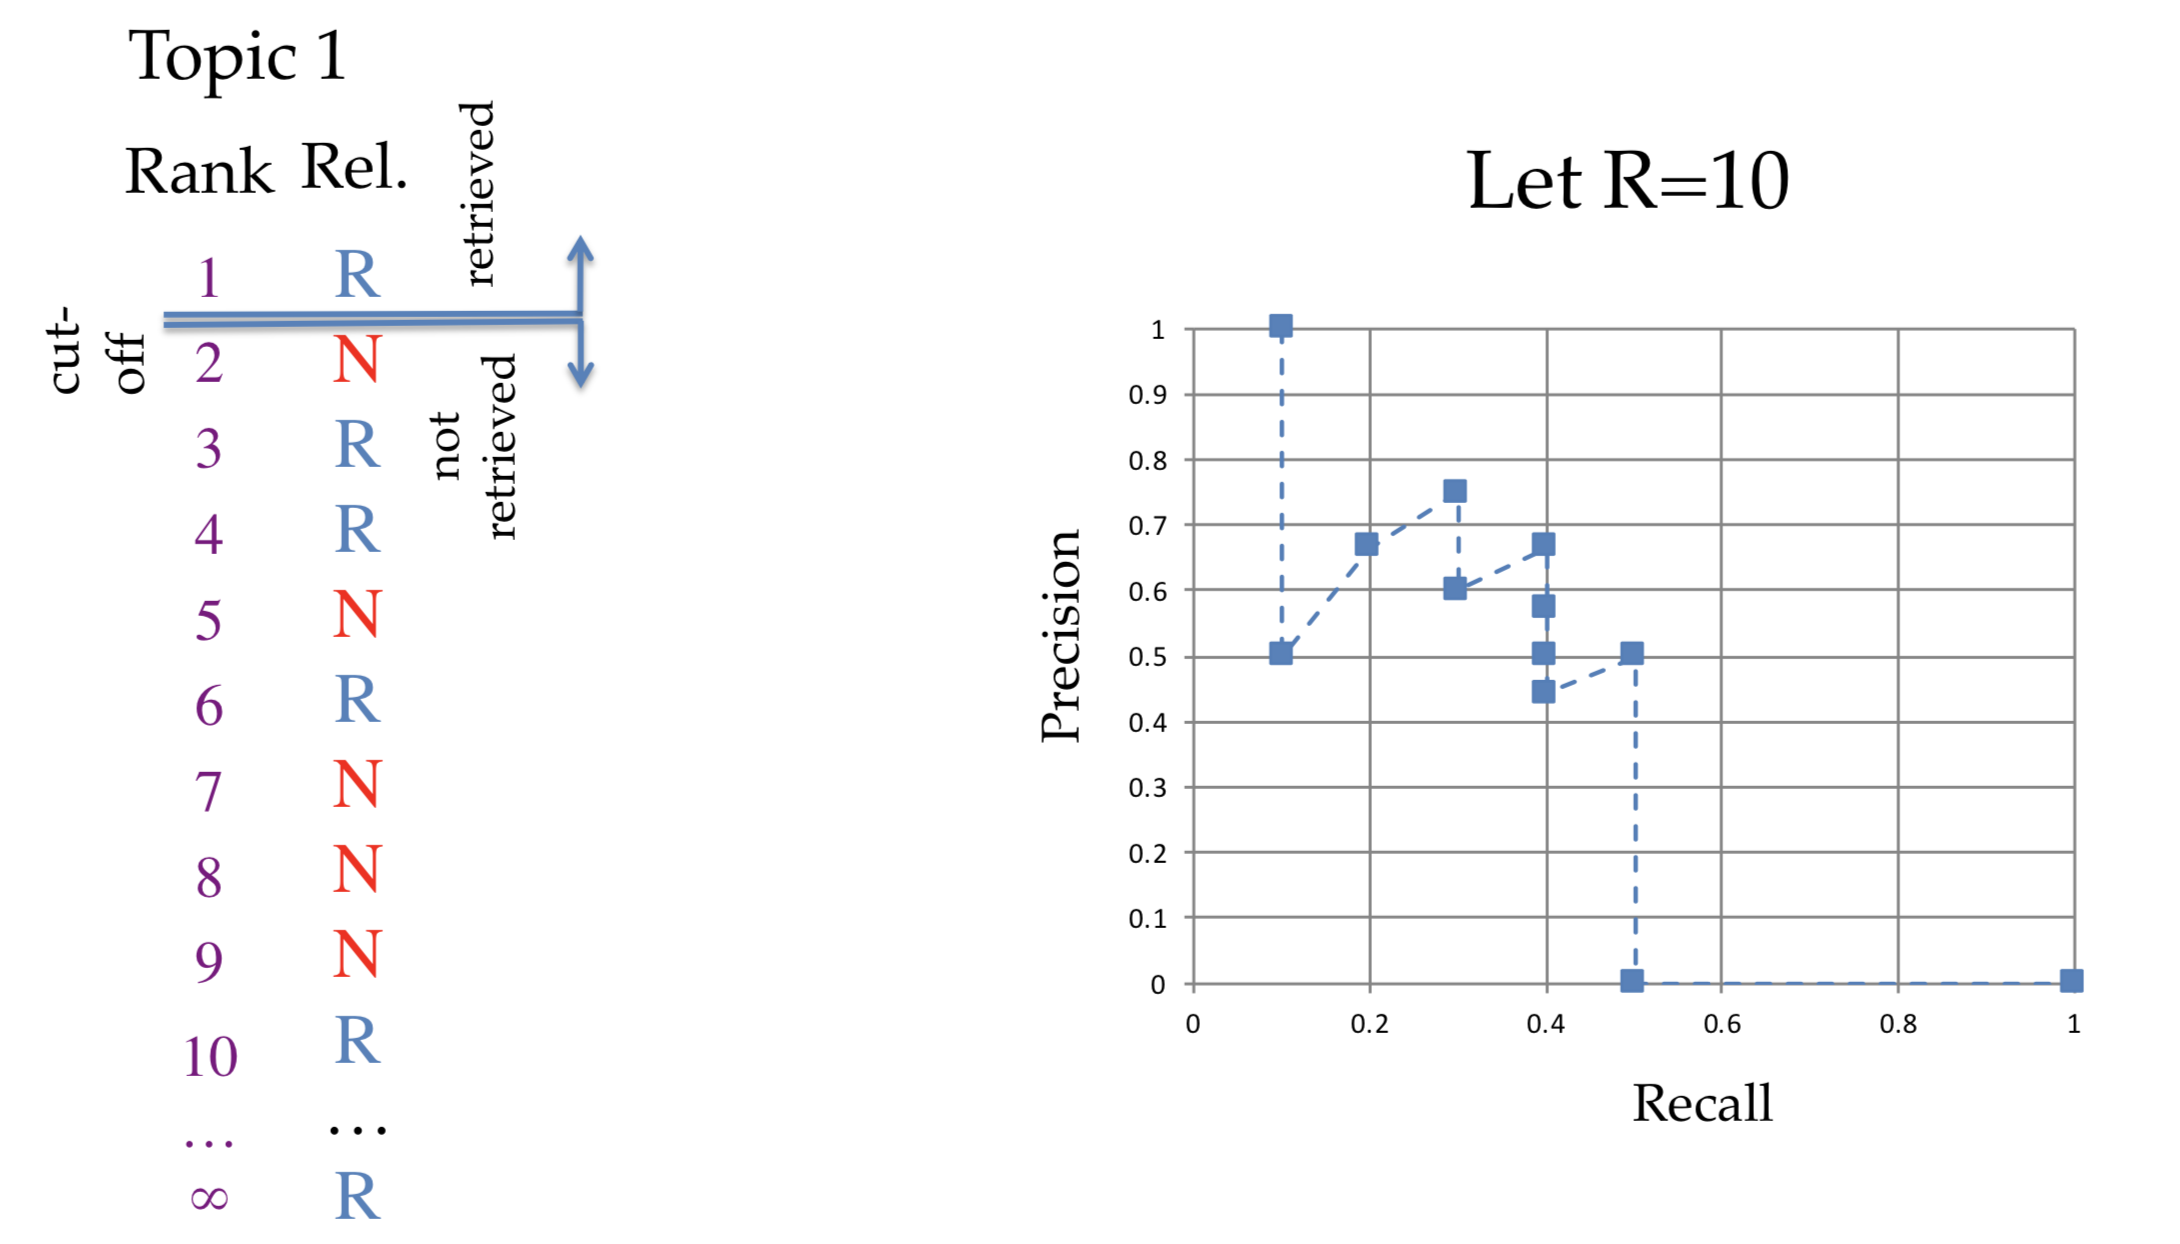
\includegraphics[width=0.4\textwidth]{figures/offline_eval_RP_curves.png}
		\caption{R/P curves for ranking}
		\label{img:offline_eval_RP_curves}
	\end{figure}
	\item When having multiple queries, we would average the RP curves. 
	\item The area under the curve is the average precision which can also be calculated by taking the average of all precision values at ranks with relevant documents.
	\item Usually, a binary scale of whether a document is relevant is not sufficient. For a graded relevance scale, we can use different evaluation measures
	\begin{itemize}
		\item \textbf{Discounted Cumulative Gain (DCG)} - considers the relevance grade and position of every document. The total gain is accumulated at a certain rank $k$:
		$$DCG@k = \sum\limits_{\text{rank} r=1}^{k} \frac{2^{\text{rel}_r} - 1}{\log_2\left(1 + r\right)}$$
		\item The numerator is the non-linear relevance score of the document at rank $r$, and the denominator the discount over ranking position
		\item The score highly depends on the best possible ranking for a query. Thus, the DCG can be normalized by the value of the best ranking $\implies$ $0\leq nDCG \leq 1$. This makes it easier to compare scores over different queries
	\end{itemize}
\end{itemize}
\subsubsection{Model-based Evaluation measures}
\begin{itemize}
	\item Another perspective of evaluation is looking at different aspects of possibles metrics. A model-based approach considers the following three components:
	\begin{enumerate}
		\item \textbf{Browsing model} - describes how the user interacts with results, like the probability of a document being clicked/viewed $\Rightarrow p(d)$
		\item \textbf{Model of document utility} - describes how a user derives utility from individual relevant documents. Similar to how to determine the graded relevance scale $\Rightarrow g(d)$.
		\item \textbf{Utility accumulation model} - describes how a user accumulates utility in the course of browsing $\Rightarrow E\left[g(D)\right] = \sum_{r=1}^{\infty}g(d) \cdot p(d)$
	\end{enumerate}
	\item Examples for the browsing models
	\begin{itemize}
		\item \textit{Position-based models} - the chance of observing a document depends on the position in the ranking. We can for example model it by $\Rightarrow p(d_r)=(1-\theta)^{r-1} \theta$. The corresponding utility accumulation is described by Rank-biased Precision (RBP): $RBP = \sum_{r=1}^{\infty}\text{rel}_r (1-\theta)^{r-1} \theta$
		\item \textit{Cascade-based models} - considers $\theta$ as a function of the document at rank $r$. Mostly, the following function is used: $\theta_r = \mathcal{R}(\text{rel}_r) = \frac{2^{\text{rel}_r}-1}{2^{\text{max rel}}}$. The corresponding utility accumulation is the \textit{Expected Reciprocal Relevance}: $ERR@k = \sum\limits_{r=1}^{k} \frac{1}{r} \cdot \theta_r \cdot \prod\limits_{i=1}^{r-1}\left(1 - \theta_i\right)$
	\end{itemize}
\end{itemize}
\subsubsection{Collection construction}
\begin{itemize}
	\item To evaluate a system offline, we need labels of whether a document is relevant with respect to a query (or graded scale) $\Rightarrow$ labels are created by humans
	\item First step is to generate a huge document collection, and generate a set of topics/queries that should be evaluated. Mostly, queries are selected from very frequent, common and rare query bin sets of highly-used search engines 
	\item To be able to calculate measures like recall, we need to find all relevant documents in the collection. Can be done either deterministically or stochastically
	\begin{itemize}
		\item \textbf{Depth-k pooling} - deterministic, standard method. Apply $M$ IR systems and take the union of the $k$ top results of all $M$ systems. This set of documents is labeled by humans, and all others are considered as not relevant. Note that we need the $M$ systems to be different/take another perspective on the data so that they don't find all the same documents. Otherwise, future IR algorithms can find relevant documents that the others haven't found yet and will be punished for that. $k$ is task specific, but a value of $100$ has shown to be sufficient
		\item \textbf{Random Sampling} - stochastic method. Simplest approach is for a query $q$, just sample a small set of documents out of the whole corpus and label those. Otherwise are considered as unlabeled, thus neglected in evaluation. Problem: significant sparsity of relevant documents in the corpus. 
	\end{itemize}
\end{itemize}
\subsection{Challenges of offline evaluation}
\label{sec:offline_eval_problems}
\begin{itemize}
	\item Expensive and slow to collect new data
	\item Ambiguous queries are particularly hard to judge realistically (what intent is most popular?). Particularly hard for personalized searches
	\item Judges need to correctly appreciate uncertainty/allow different intents
	\item How to identify when relevance changes (temporal, query intent changes, ...)?
\end{itemize}
\subsection{Comparative evaluation}
\begin{itemize}
	\item How do we compare different retrieval systems? Is the difference only due to random noise? $\implies$ Statistical significance test
	\item Two hypotheses where we want to prove that $H_0$ is wrong: $$H_0: \text{MAP}_E - \text{MAP}_P = 0, \hspace{4mm} H_1: \underbrace{\text{MAP}_E - \text{MAP}_P \neq 0}_{\text{two-sided}} \text{\hspace{2mm}or\hspace{2mm}}\underbrace{\text{MAP}_E - \text{MAP}_P > 0}_{\text{one-sided}}$$
	\item Compute the $p$-value that describes the probability of observing the test data given that $H_0$ is valid (low $p$-value disprove null hypothesis)
\end{itemize}
\subsubsection{Student's t-test}
\begin{itemize}
	\item Statistic: $$t=\frac{\mu_{E-P}}{\frac{\sigma_{E-P}}{\sqrt{N}}} = \frac{\overline{AP_E - AP_P}}{\frac{\sigma_{E-P}}{\sqrt{N}}}$$
	\item We assume that the mean measure follow a normal distribution (see Figure~\ref{img:hypothesis_testing_t_test_t_dist})
	\begin{figure}[ht]
		\centering
		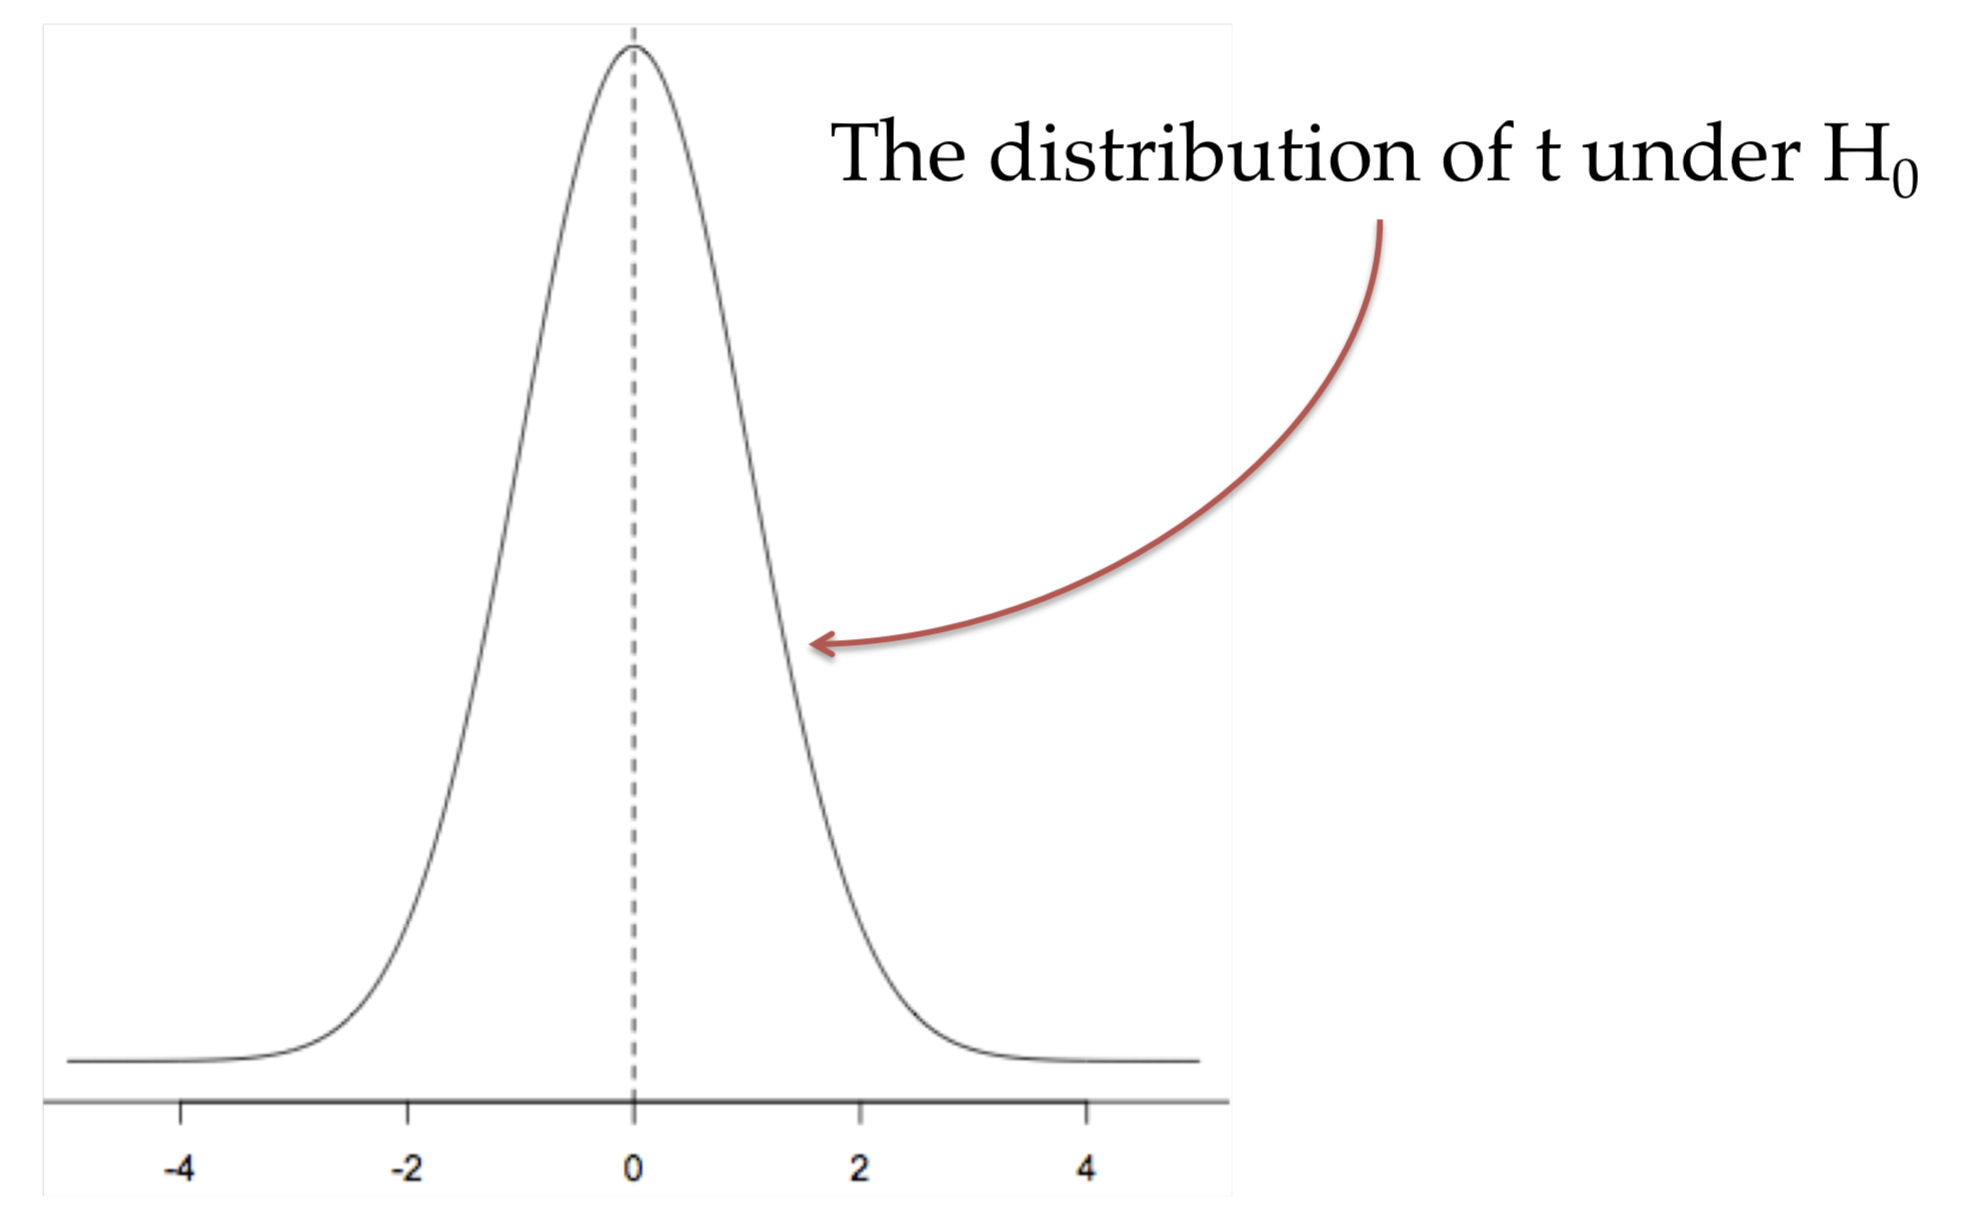
\includegraphics[width=0.3\textwidth]{figures/hypothesis_testing_t_test_t_dist.png}
		\caption{Distribution of $t$ values under the null hypothesis}
		\label{img:hypothesis_testing_t_test_t_dist}
	\end{figure}
	\item The $p$-value is determined by the area under the distribution right from the determined value
	\item If the $p$-value is lower than the significance level $\alpha$, reject null hypothesis
	\item There are two different error types for the t-test: 
	\begin{description}
		\item[Type 1] rejecting null hypothesis although it was true (prob. is $\alpha$)
		\item[Type 2] not rejecting the null hypothesis although it was false (prob. is $\beta$)
	\end{description}
	\item There are four aspects of the test that interact with each other. If one is unknown, it can be derived from the others
	\begin{enumerate}
		\item \textit{Sample size} $N$
		\item \textit{Effect size} = diff. of means / std. dev.
		\item \textit{Significance level} = Type 1 error $\alpha$
		\item \textit{Power} = 1 - Type 2 error $\beta$. Prob. of finding an effect if it is there. 
	\end{enumerate}
\end{itemize}
\subsubsection{Sign test}
\begin{itemize}
	\item Look at score/sample pairs from $A$ and $B$ and consider the null hypothesis $H_0: P(B>A)=P(A>B)=1/2$.
	\item It is a discrete way of looking at the t-test. For a sample size of $N$, we get a binomial distribution with $N$ bins. The bins summed up from the measured number of $B$ winning over $A$ describe the p-value (see Figure~\ref{img:hypothesis_testing_sign_test})
	\begin{figure}[ht]
		\centering
		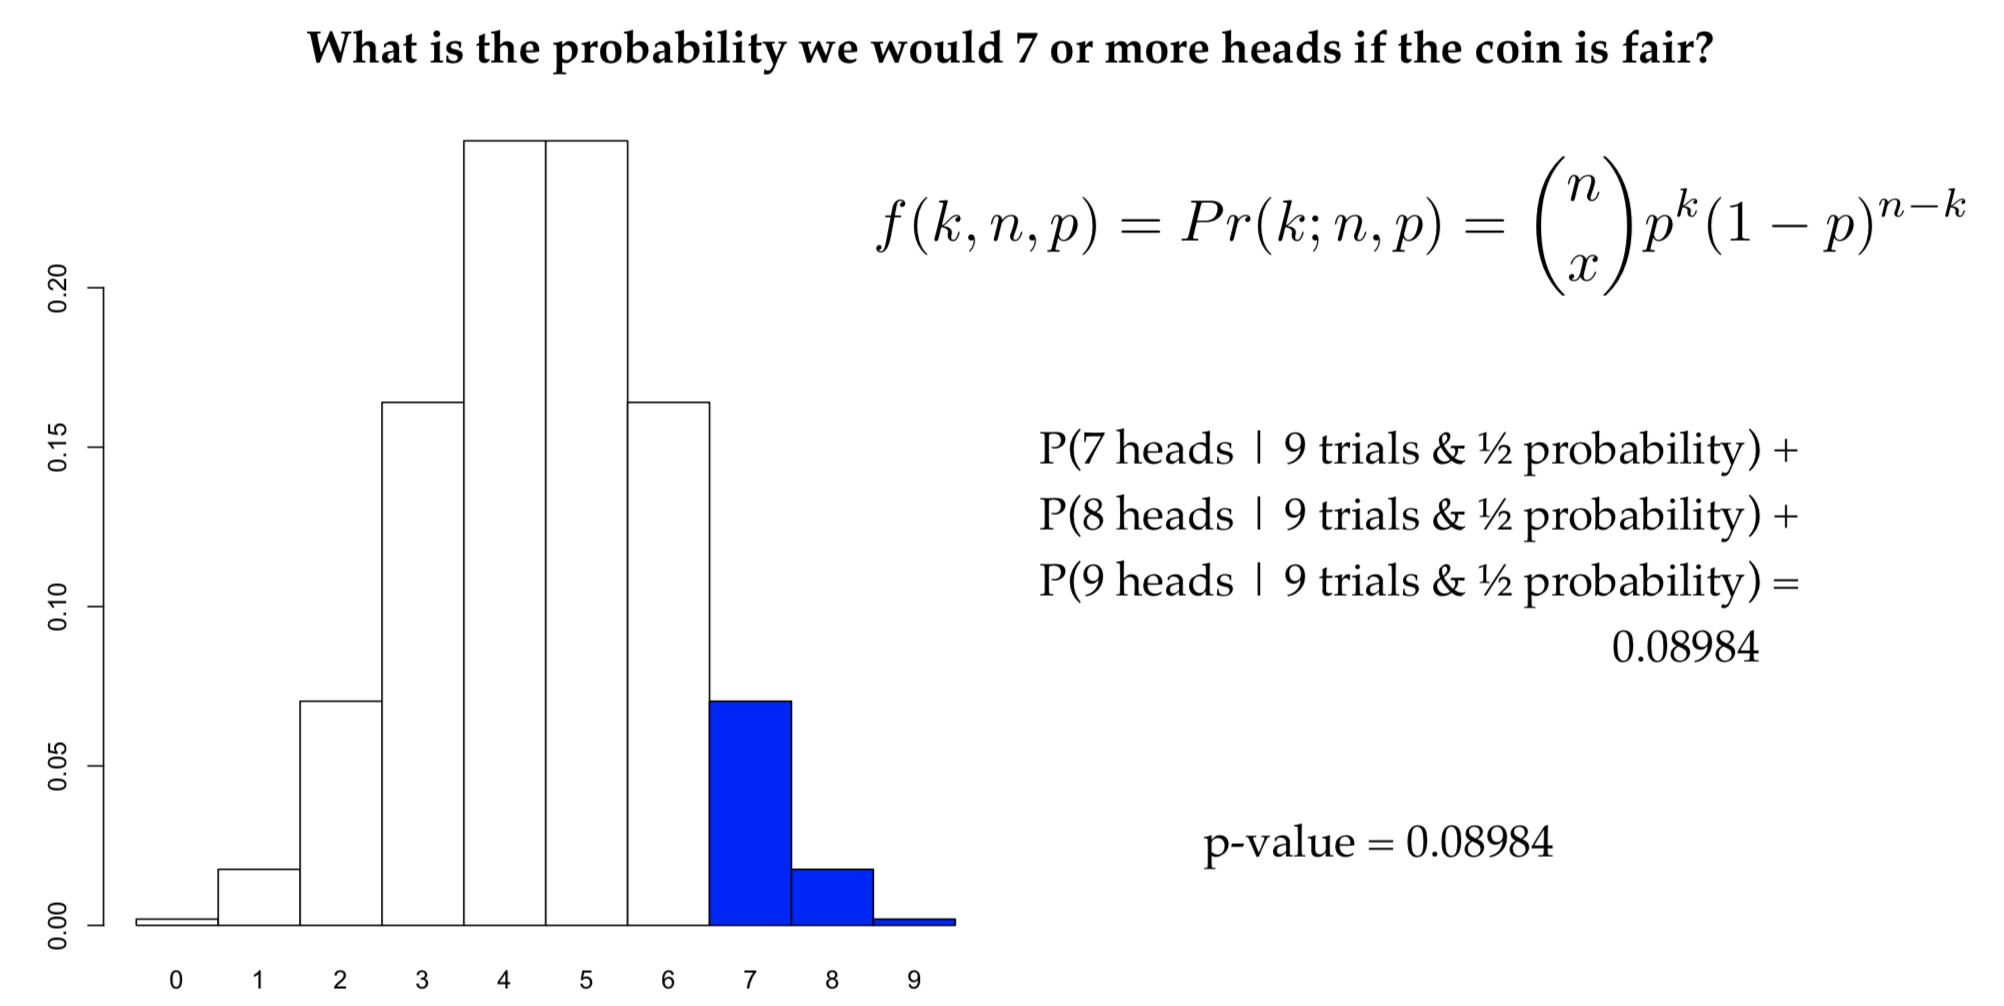
\includegraphics[width=0.4\textwidth]{figures/hypothesis_testing_sign_test.png}
		\caption{Distribution of $t$ values under the null hypothesis}
		\label{img:hypothesis_testing_sign_test}
	\end{figure}
\end{itemize}
\subsubsection{Distribution-free tests}
\begin{itemize}
	\item Tests where we do not explicitly assume the underlying data to be sampled from a specific distribution
	\item \textbf{Randomization test}
	\begin{itemize}
		\item Given: a set of results for $N$ queries for algorithm $A$ and $B$
		\item Repeat for many times:
		\begin{itemize}
			\item Randomly swap values for a query in algorithm $A$ and $B$
			\item Compute average of both systems and their difference
			\item Add difference to an array
		\end{itemize} 
		\item The two systems are significantly different, if the actual difference without swapping is outside 95\% of the differences in the array.
	\end{itemize}
	\item \textbf{Bootstrap test}
	\begin{itemize}
		\item Same preparation as for randomization test
		\item Repeat for many times:
		\begin{itemize}
			\item Randomly sample pair of scores (i.e. selecting queries) of $A$ and $B$ with replacement
			\item Compute average of each systems in the set of pairs
			\item Add difference to an array
		\end{itemize}
		\item The two systems are significantly different if the mean of the array can be shown to be significantly different from 0.
	\end{itemize}
	
\end{itemize}
\section{Online evaluation}
\begin{itemize}
	\item In online evaluation, the system interacts with the user $\implies$ user "tells" what is relevant, system analyzes the user's behavior for gaining that knowledge
	\item The benefit of online evaluations is that they are mostly simpler and directly incorporate measuring the ranking quality
	\item However, the downsides are that the results are worse to explain/interpret (why did users click less, different queries might rely on different metrics, ...). Also, evaluations might not be comparable over time so that we also need to ensure the same conditions/user population for both systems.
\end{itemize}
\subsection{Analyzing user behavior}
\begin{itemize}
	\item A user provides various signals from which we can try to retrieve his "happiness" about the results. The following ones are mostly used:
	\item \textit{Clicks} - clicks are mostly noisy so that a click doesn't ensure that the document was actually relevant. Clicks have several biases:
	\begin{itemize}
		\item \textit{Position bias} - a user tends towards clicking higher ranked results
		\item \textit{Contextual bias} - nearby results effect the click probability of a document
		\item \textit{Attention bias} - some results draw more attention to themselves by the usage of images, font size, ...
	\end{itemize}
	\item \textbf{Time} - the time a user spends on a certain query before coming back to search engine
	\begin{itemize}
		\item \textit{Dwell time} - time spent on a clicked page. If duration is more than 30 seconds, we assume that click satisfied
		\item \textit{Exit type} - how the user exists the page (closing browser, continue scrolling through results, putting in new query, ...) 
	\end{itemize}
	\item \textit{Mouse movement} - time on website is not sufficient. Mouse movement can indicate whether user is actually reading or only scrolling/scanning
	\item \textit{Reformulations} - if new query is entered, check for similarity with the previous one. Reformulated/Similar queries that were entered quickly after the first one, indicate that user was not satisfied with previous results.
\end{itemize}
\subsection{A/B Testing}
\begin{itemize}
	\item When testing two systems in an online experiment, we need to make sure that both have the same preconditions so that the system improvements clearly correlate with the new click/sale numbers
	\item In A/B Testing, users are split into two groups where each group is assigned to one of the algorithms. We analyze the users' behavior on both systems and calculate a metric based on that. Comparing the results for both systems on significance leads to a final decision.
	\item \textit{Challenges} in A/B Testing
	\begin{itemize}
		\item If one system is very different and probably bad, it will affect the \textit{user experience} and damages website image $\implies$ perform offline evaluation in advance to avoid testing a very bad system
		\item It is hard to define \textit{metrics} as they can contradict each other. For example, if we report number of clicks and sessions per users, a click increase can indicate better/more relevant results. However, if another systems provides snippets that already contain the information, the user will click less.
		\item The metric should be as sensitive as possible. \textit{Sensitivity} is the ability of the metric to detect the statistically significant difference when the treatment effect exists $\implies$ how many queries/days/users/... for significance needed?
	\end{itemize}

	\begin{figure}[ht]
		\centering
		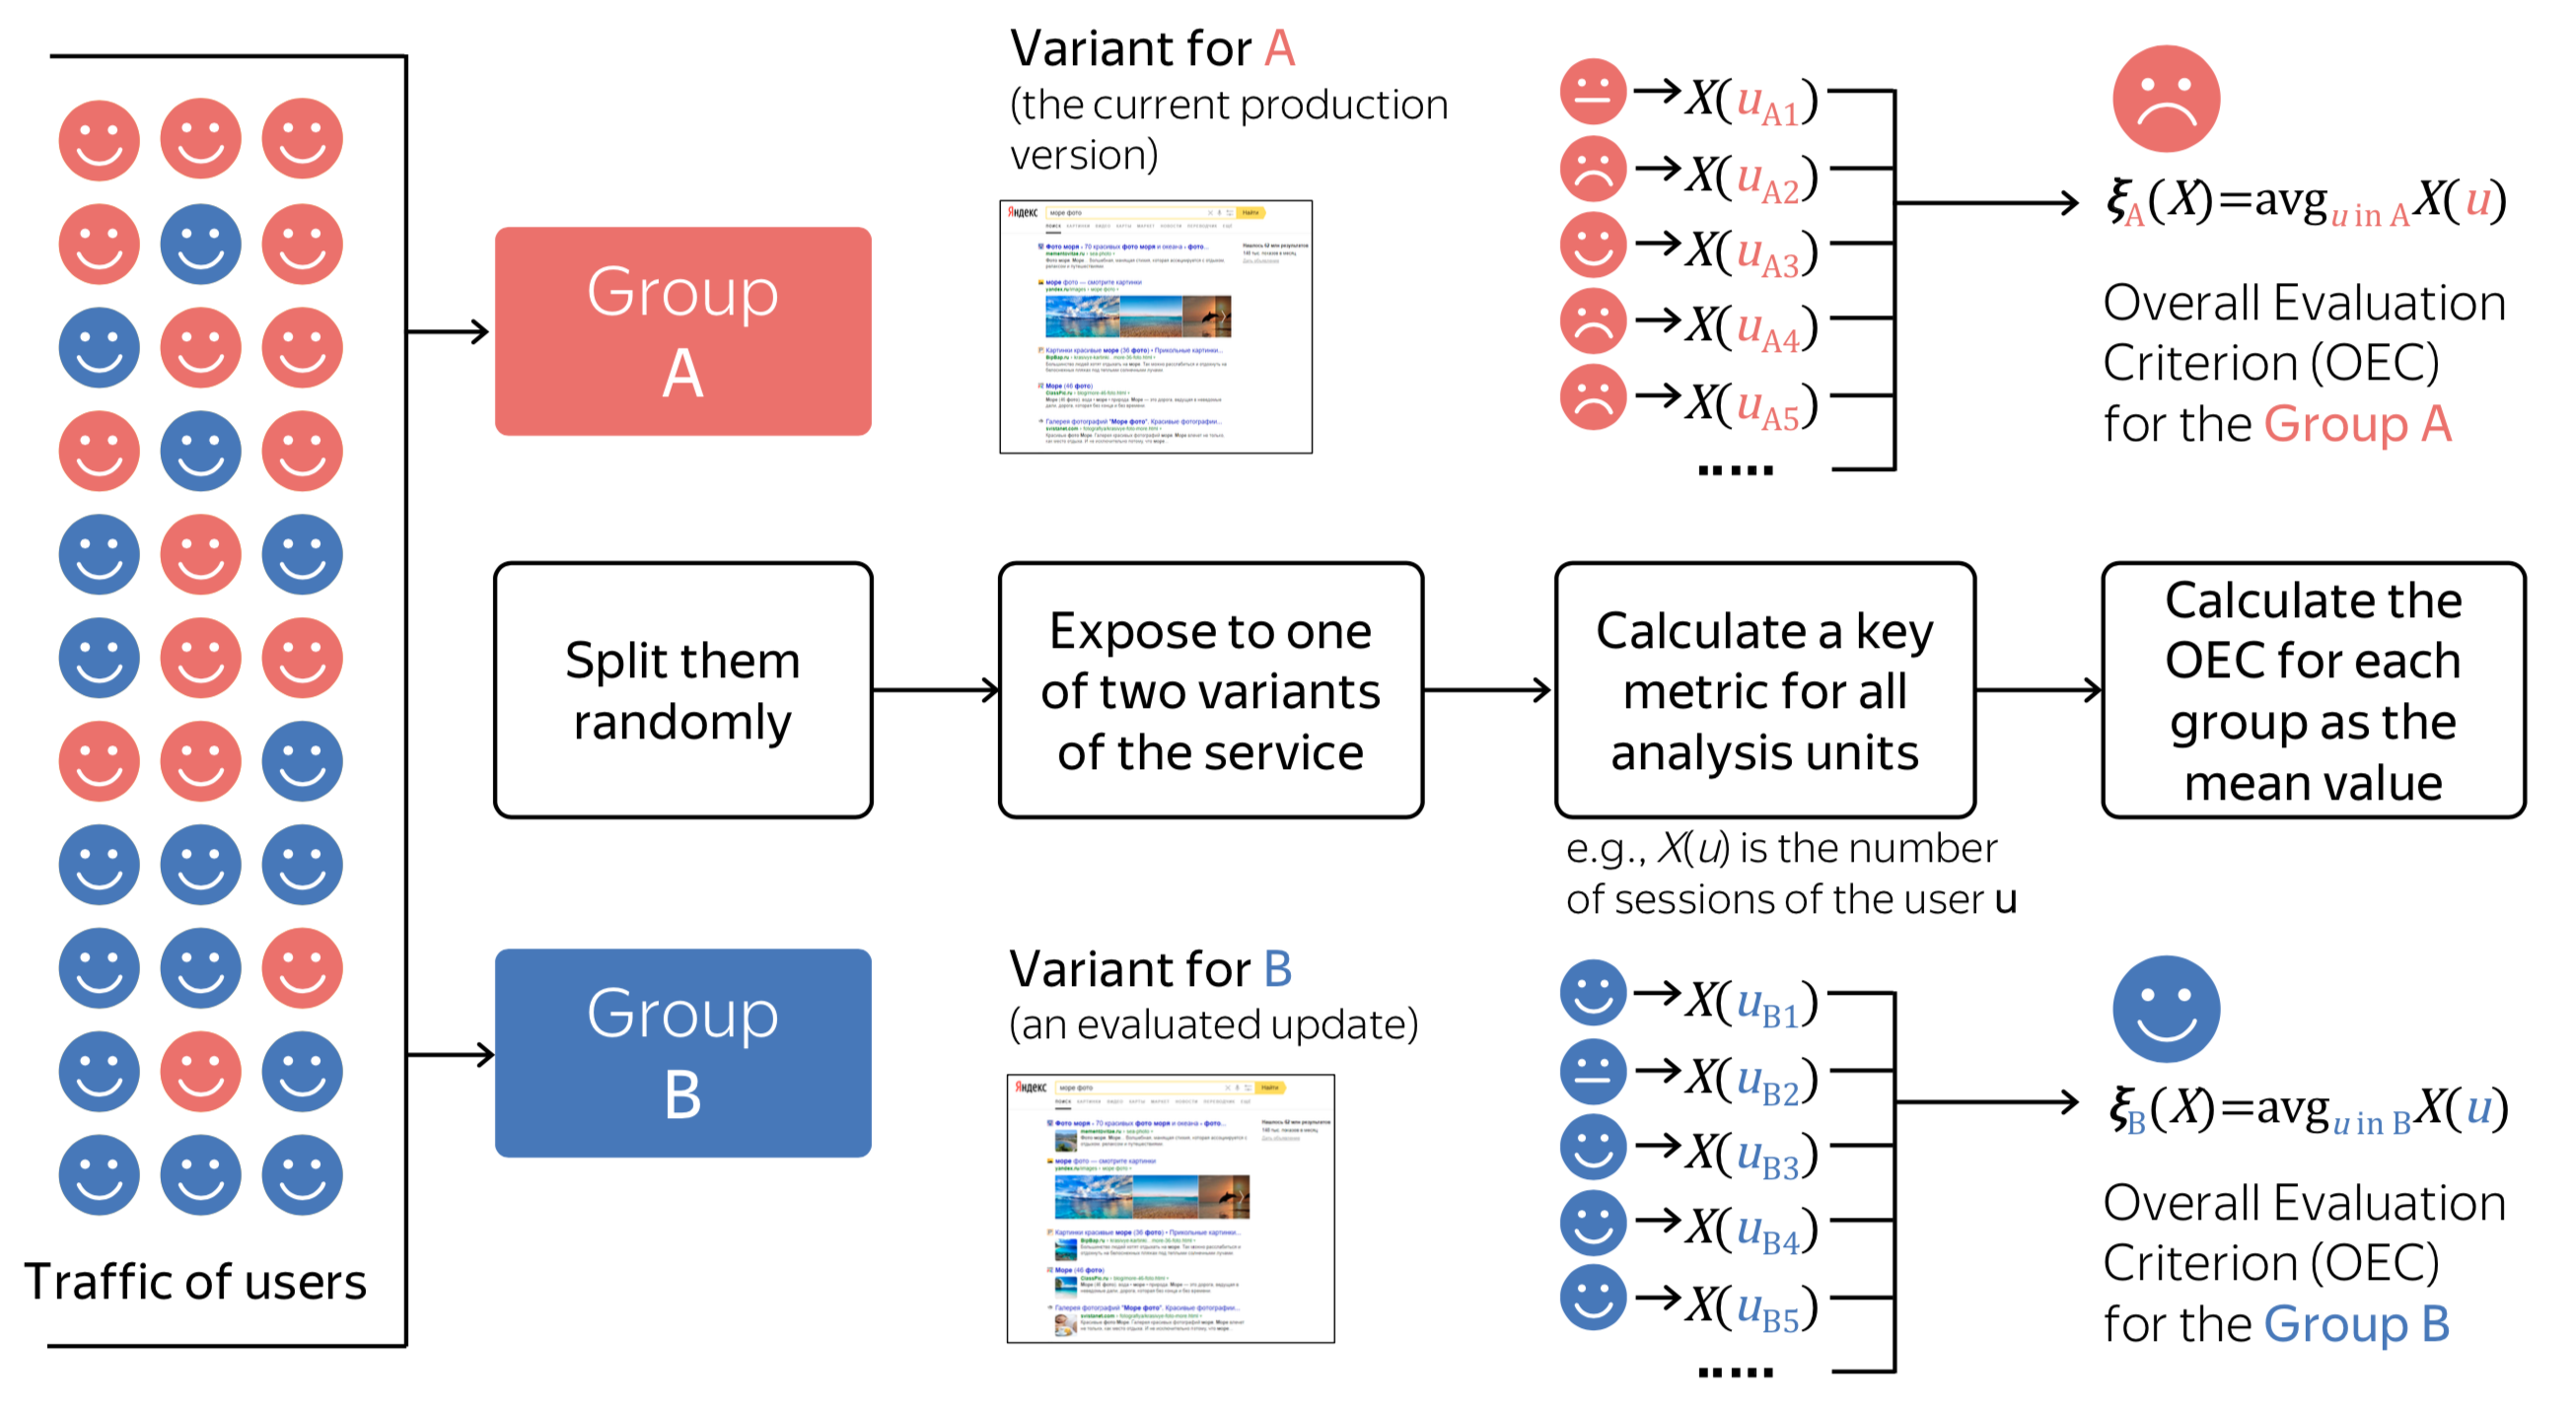
\includegraphics[width=0.5\textwidth]{figures/online_eval_AB_testing.png}
		\caption{Visualization of A/B Testing}
		\label{img:online_eval_AB_testing}
	\end{figure}
\end{itemize}
\subsection{Interleaving}
\begin{itemize}
	\item A/B testing introduces a high variance by letting different users evaluate different systems $\implies$ Show interleaved results from both algorithms A and B without telling the user which document is from which model
	\item The evaluation is based on the clicks of a user where the algorithm gets the credit that provided the clicked document
\end{itemize}
\subsubsection{Balanced interleaving}
\begin{itemize}
	\item In balanced interleaving, we select randomly which algorithm starts (A or B). If A would start, we take the first document of A and place it in our interleaved ranking list. Then we pick the first document of B and continue with A again
	\item If a document is already in the interleaved ranking, we skip this document and continue with picking the next document from the \textit{other} ranking model 
	\begin{figure}[ht]
		\centering
		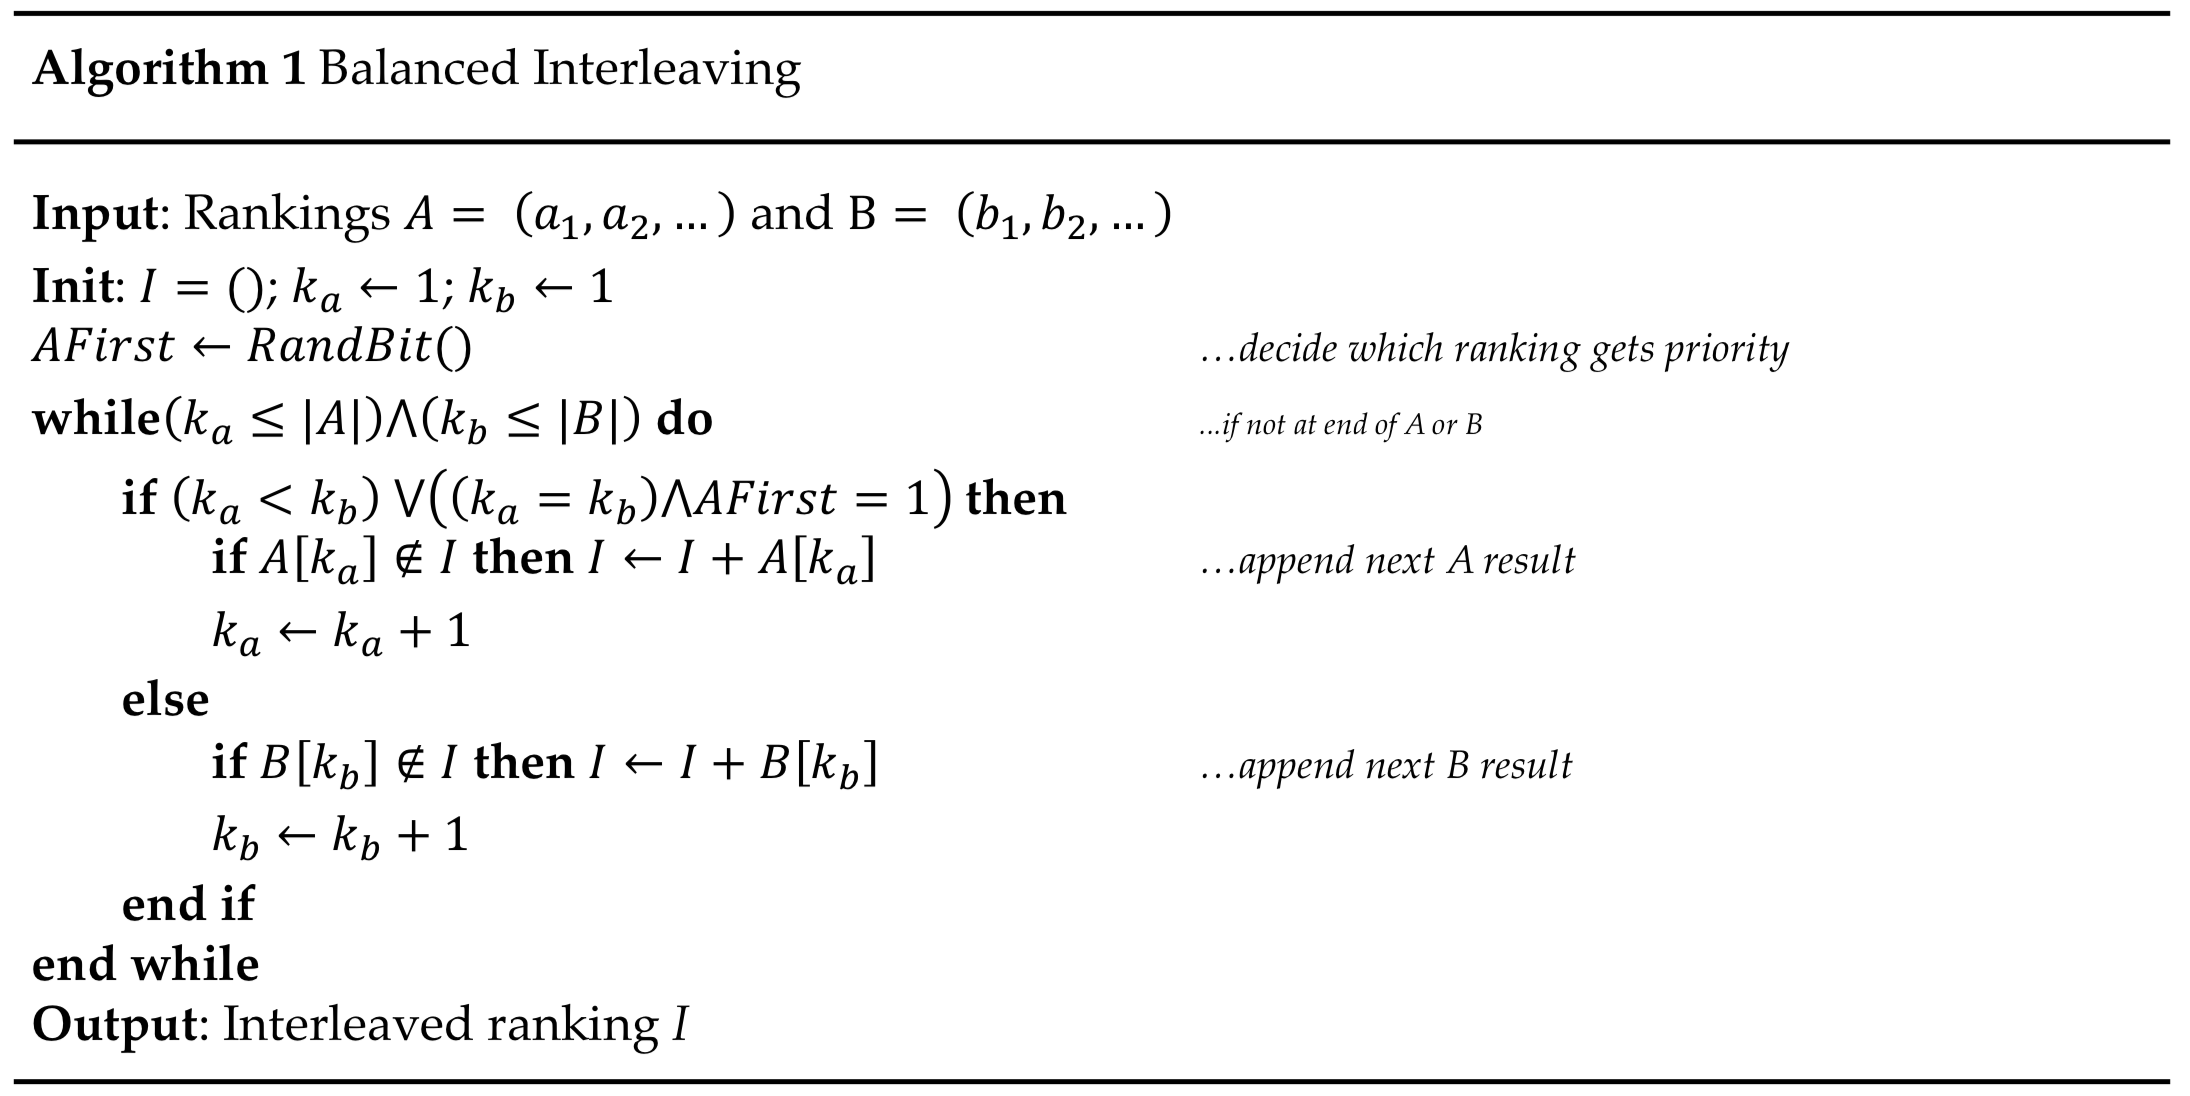
\includegraphics[width=0.5\textwidth]{figures/online_eval_balanced_interleaving.png}
		\caption{Formal algorithm describing balanced interleaving}
		\label{img:online_eval_balanced_interleaving}
	\end{figure}
	\item Problem: balanced interleaving brakes under corner cases. Assume following ranking:
	$$A: \left\{d_1, d_2, d_3, d_4\right\}, B: \left\{d_2, d_3, d_4, d_1\right\}$$
	No matter whether we start at model A or B, the interleaved list contains three documents assigned to B and only one to A. Thus, random clicking would lead to B winning $\implies$ bias. Resolved by team-draft interleaving
\end{itemize}
\subsubsection{Team-draft interleaving}
\begin{itemize}
	\item In team-draft interleaving we guarantee that both algorithms contribute equally to the interleaved ranking
	\item At each stage, we flip a coin to determine whether to pick the next document from A or B first. Afterwards, the document of the other system is picked
	\item If a document is already in the interleaved ranking, we look for the next document from the \textit{same} ranking model until we find a new document.
	\begin{figure}[ht]
		\centering
		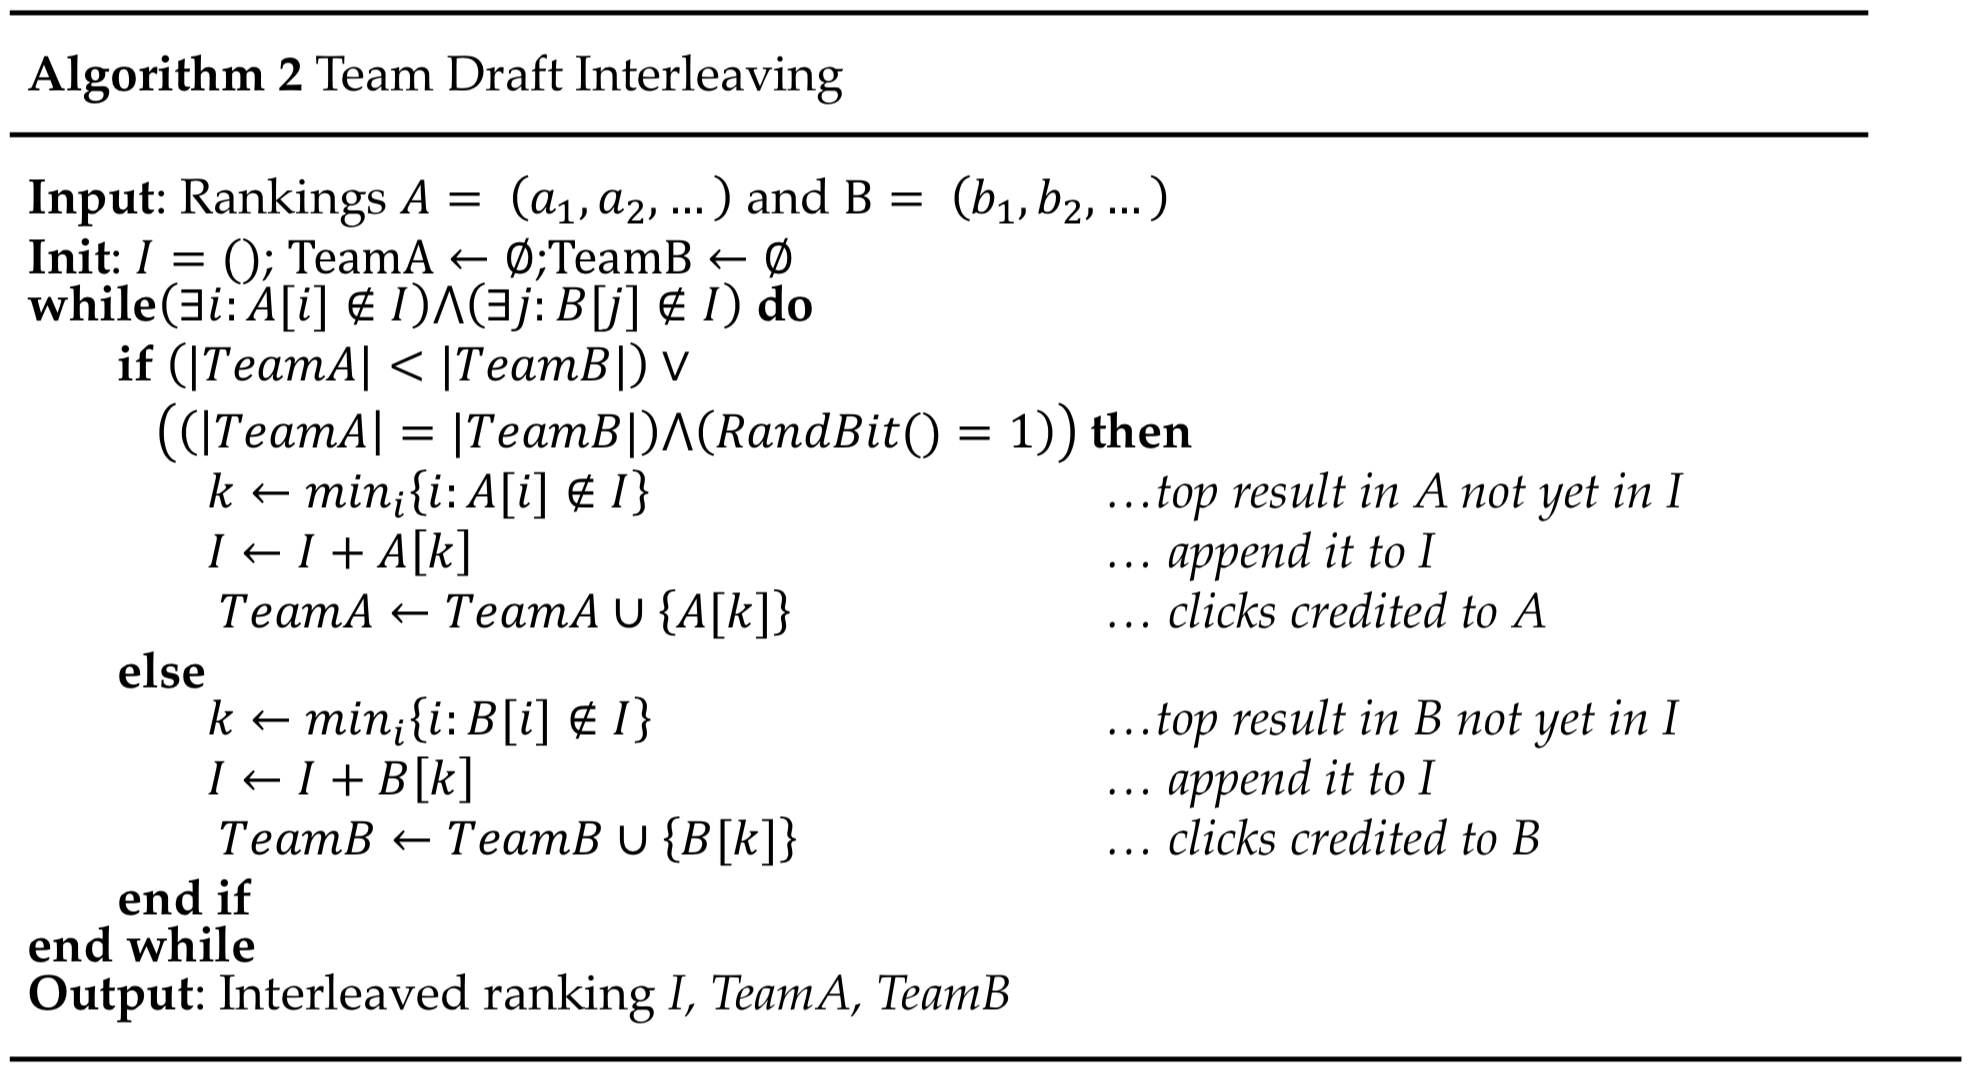
\includegraphics[width=0.5\textwidth]{figures/online_eval_team_draft_interleaving.png}
		\caption{Formal algorithm describing Team-draft interleaving}
		\label{img:online_eval_team_draft_interleaving}
	\end{figure}
	\item There are also corner cases that can cause troubles in team-draft interleaving. However, in practice this rarely happens/has a significant effect. 
\end{itemize}
\subsubsection{Probabilistic interleaving}
\begin{itemize}
	\item To avoid biases completely, we can apply probabilistic models
	\item Convert the ranking of each model to a probability distribution by applying softmax ($\tau = 3$):
	$$p_i(d) = \frac{\frac{1}{r_i(d)^{\tau}}}{\sum_{d' \in D} \frac{1}{r_i(d')^{\tau}}}$$
	\item For every position in the interleaved ranking, flip a coin to determine whether to pick a document from A or B. Next, we sample from the corresponding softmax distribution a document without replacement, and add it to the interleaved list. The picked document is removed from the probability distributions of A and B. 
	\item We can perform evaluation by counting the clicks for documents sampled from A and B. We expect the same number of clicks for documents at the same position of both algorithms due to the same probability in the softmax. % both A and B based on the softmax, and compare which one has the higher probability sum of all clicked documents. Thus, for documents at the same rank, we expect a tie.
	\item Note that compared to a hard assignment of 0 or 1 in balanced and team draft interleaving, the distribution of credit accumulated for clicks is smoothed based on the relative rank of the document in the original result lists (a click on any document leads to a non-zero credit for both rankings)
	\item The algorithm is summarized in Figure~\ref{img:online_eval_probabilistic_interleaving}
	\begin{figure}[ht]
		\centering
		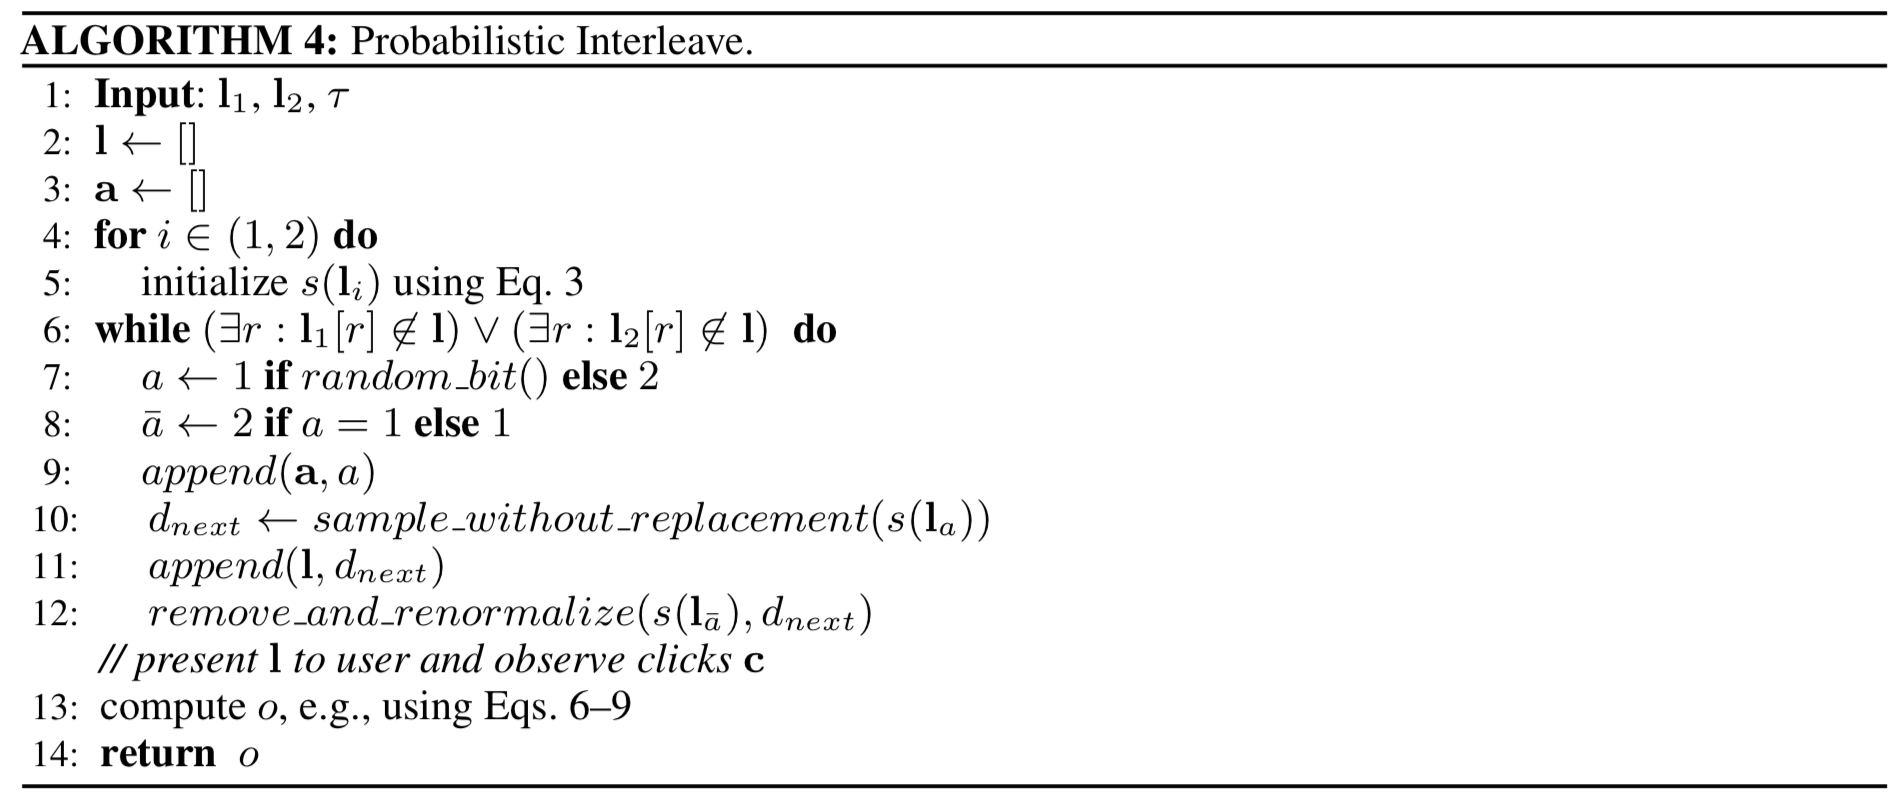
\includegraphics[width=0.5\textwidth]{figures/online_eval_probabilistic_interleaving.png}
		\caption{Formal algorithm describing probabilistic interleaving}
		\label{img:online_eval_probabilistic_interleaving}
	\end{figure}
	\item Another, more efficient evaluation method is by marginalizing over all possible assignments $a$. Therefore, we calculate the probability of the interleaved list $l$ given $a$ (and the query $q$) by successively multiplying the softmax probabilities at that point. For example, the first assignment $a=\left\{1,1,1,1\right\}$ leads to the following calculation:
	$$p(l_i|a=\left\{1,1,1,1\right\},q) = 0.85 \cdot \frac{0.1}{0.15} \cdot \frac{0.03}{0.05} \cdot \frac{0.02}{0.02} = 0.34$$
	\item Normalizing all $p(l_i|a,q)$ by its sum lead to $p(a|l_i,q)$ $\implies$ $p(a|l_i,q) = \frac{p(l_i|a,q)}{\sum_{a \in A} p(l_i|a,q)}$
	\item For every assignment, we add the value $o=-1$ times the probability $p(a|l_i,q)$ if more clicked documents were assigned to $A$. If $B$ has more clicks, we use $o=1$ as factor, and ignore it for a tie (or multiply by $o=0$). Thus, our expected number of wins $B$ has more than $A$ is given by:
	$$E[O] = \sum_{a \in A} o_a \cdot p(a|l_i,q) \text{\hspace{2mm}where\hspace{2mm}} o_a = \begin{cases}
	 -1 & \text{if } c_A > c_B\\
	 0 & \text{if } c_A = c_B\\
	 1 & \text{if } c_A < c_B
	\end{cases}$$
	\item Figure~\ref{img:online_eval_probabilistic_interleaving_2} visualizes an example for probabilistic interleaving
	\begin{figure}[ht]
		\centering
		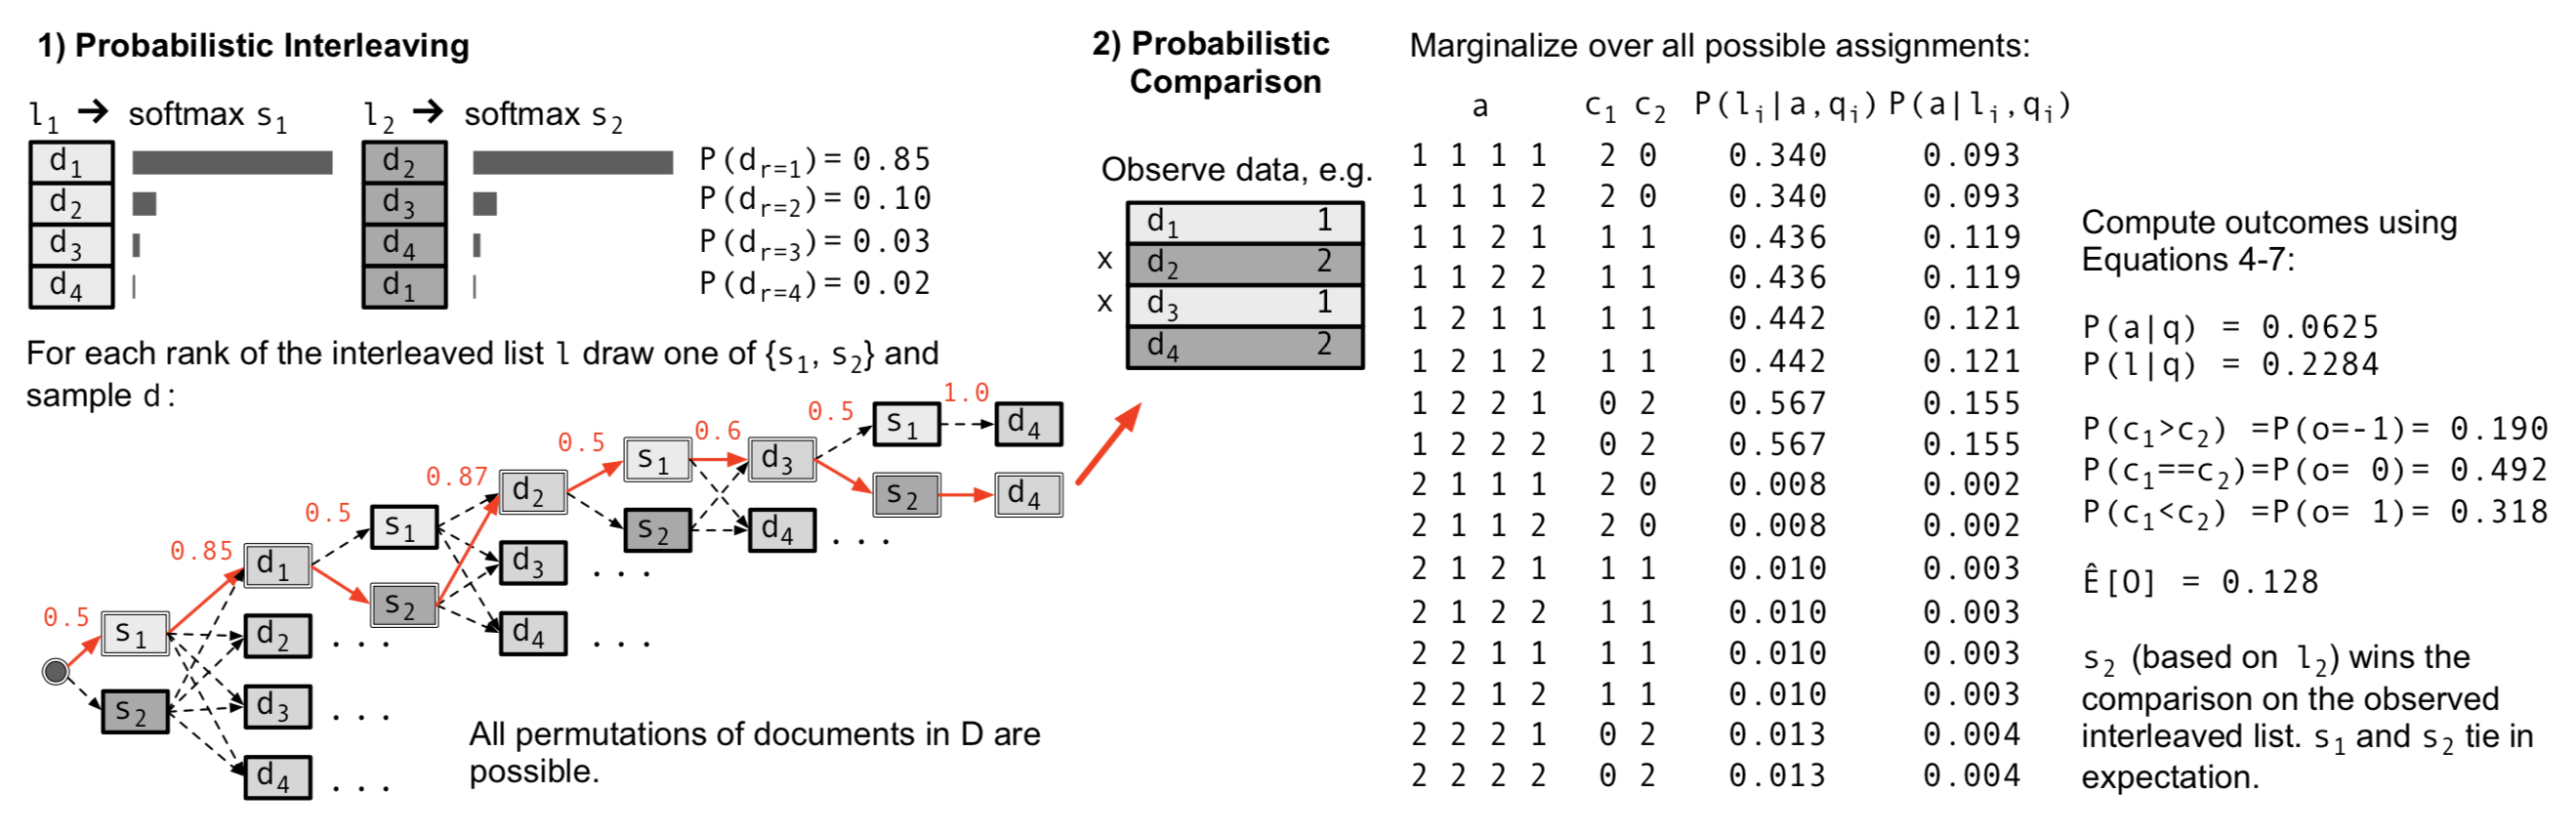
\includegraphics[width=\textwidth]{figures/online_eval_probabilistic_interleaving_2.png}
		\caption{Visualization of probabilistic interleaving}
		\label{img:online_eval_probabilistic_interleaving_2}
	\end{figure}
\end{itemize}
\section{Click models}
\begin{itemize}
	\item User clicks can be used as evaluation of IR systems as clicks indicate the relevance of a document
	\item However, clicks are highly biased (positional, textual, attention/visual,...) $\Rightarrow$ click models try to remove these biases and help using clicks for evaluation
	\item Click models are optimized/trained on click logs which record for a given query which documents were clicked
	\item Most models are based on probabilistic graphical models (PGMs) that describe the probability of a click
	\item They are mostly trained by either applying a MLE or EM algorithm
\end{itemize}
\subsection{Random click model}
\begin{itemize}
	\item In random click models, every document on the result page has the same probability of being clicked: $$P(C_u = 1) = \text{const} = \rho$$
	\item Therefore, the model contains only a single parameter, which can be optimized by applying MLE: $$\rho = \frac{\#\text{clicks}}{\#\text{shown docs}}$$
	\item \textit{Advantages}: simple and fast
	\item \textit{Disadvantages}: the random click model does not consider many aspects including the position and content of a document
	\item There are different variations of this model (also called click-through rate models - CTR) considering more aspects
	\begin{itemize}
		\item \textbf{Rank-based CTR} - modeling a probability for every rank on the result page: $P(C_{u_r} = 1) = \rho_r$
		\item \textbf{Query-document CTR} - modeling a probability for every query-document pair in the dataset: $P(C_{u}=1) = \rho_{uq}$
	\end{itemize}
\end{itemize}
\subsection{Position-based model}
\begin{itemize}
	\item Position-based models take the position \textit{and} the document-query pair into account for modeling the probability of a click
	\begin{itemize}
		\item \textit{Examination} - reading a snippet at a rank/position $\implies$ $P(E_r = 1) = \gamma_r$
		\item \textit{Attractiveness} - prob. for document-query relevance $\implies$ $P(A_{uq} = 1) = \alpha_{uq}$
		\item The combined probability of clicking on a document is therefore: $$P(C_u = 1) = P(E_{r_u} = 1) \cdot P(A_{uq} = 1)$$
	\end{itemize}
	\item The model is visualized in Figure~\ref{img:click_models_PBM_pgm}
	\begin{figure}[ht]
		\centering
		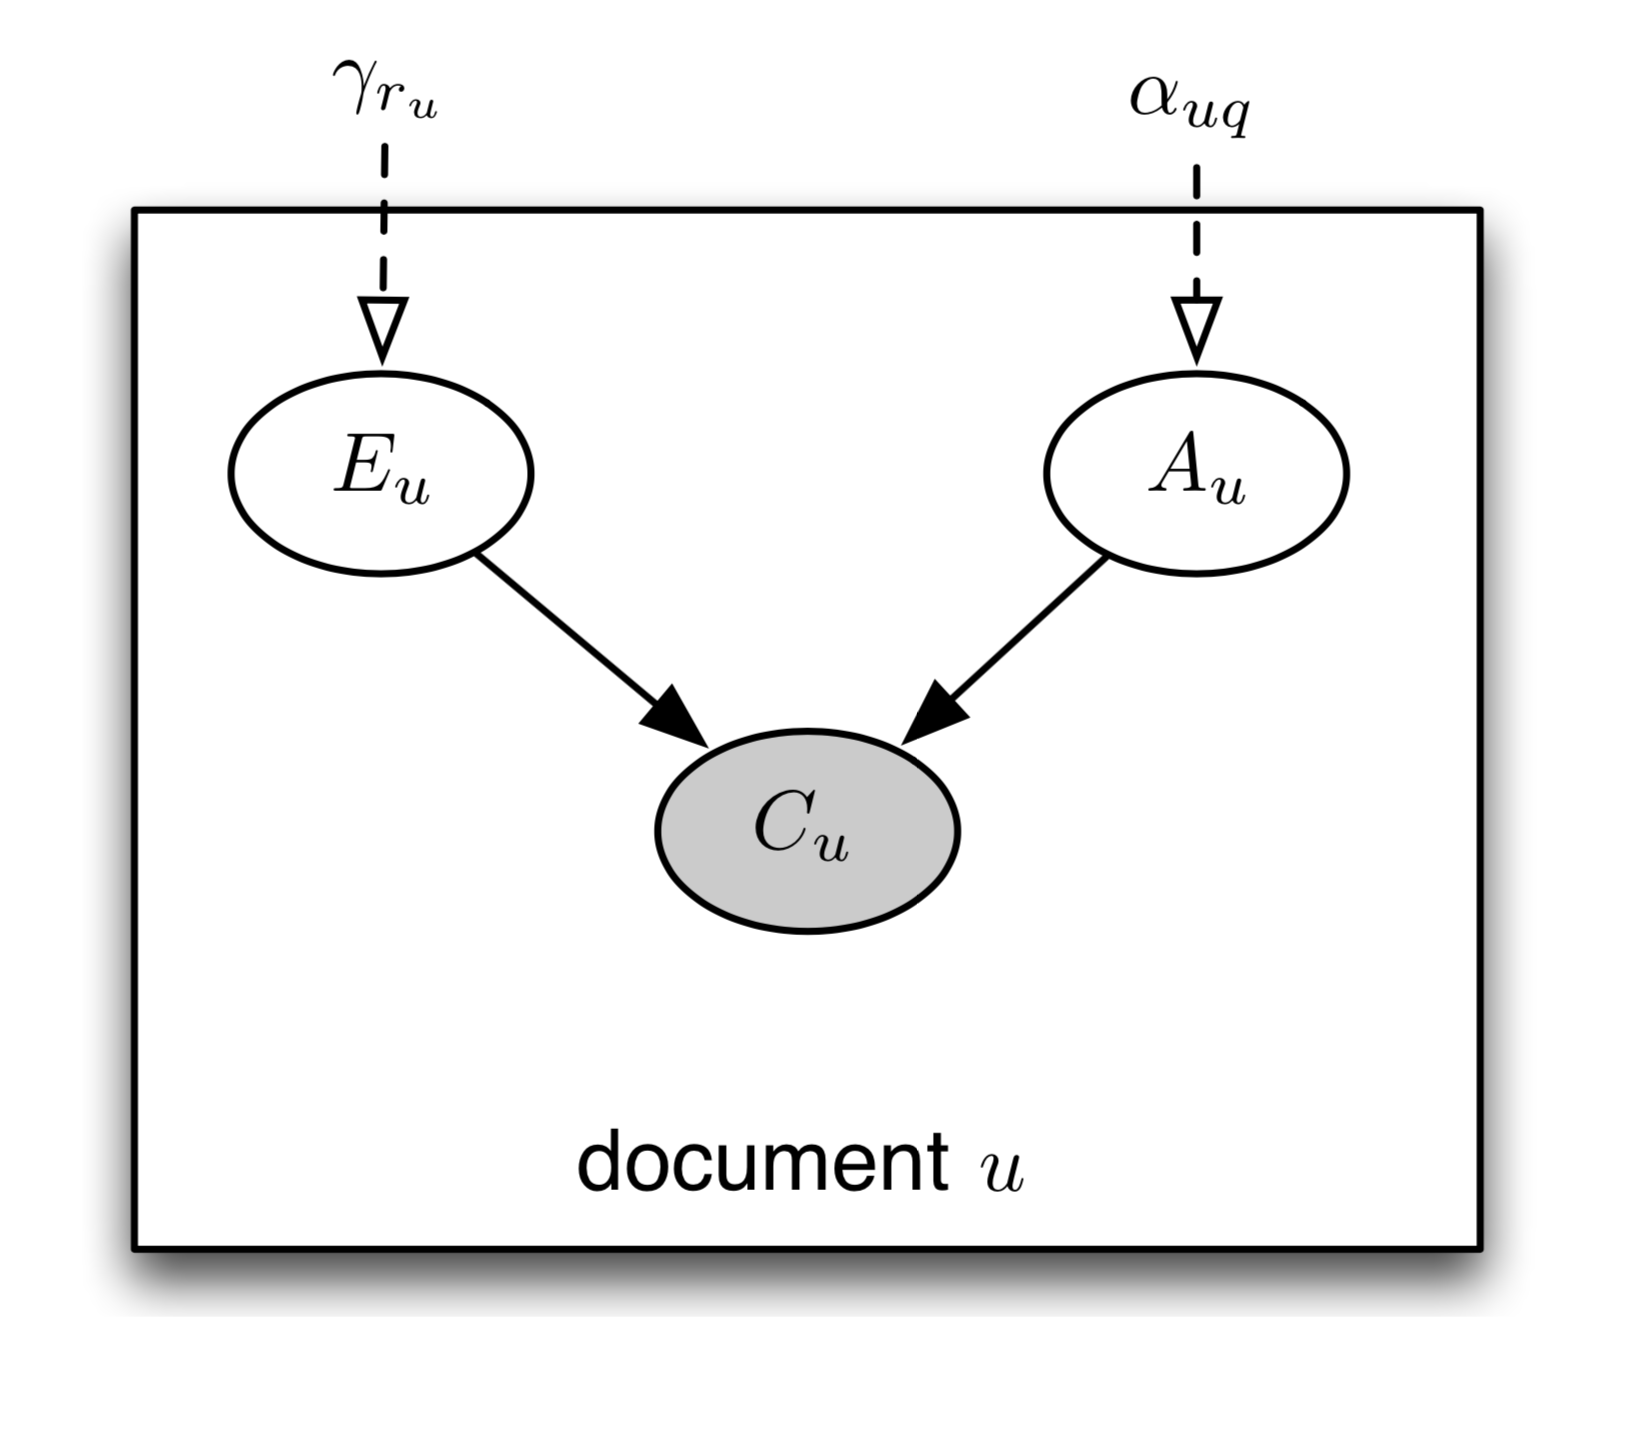
\includegraphics[width=0.25\textwidth]{figures/click_models_PBM_pgm.png}
		\caption{Probabilistic graphical model of parameters for PBM}
		\label{img:click_models_PBM_pgm}
	\end{figure}
	\item The examination models the position bias in user clicks while the attractiveness covers the document relevance
	\item \textit{Advantages}: Distinguishing between position bias and document relevance
	\item \textit{Disadvantages}: the Position-based model assumes that all clicks are independent of each other. Models that overcome this include:
	\begin{itemize}
		\item \textit{User browsing model (UBM)} - examination is also based on the rank of the previously clicked document $\implies$ $P(E_{r,r'}=1) = \gamma_{r,r'} $ ($n + n\cdot (n-1)/2$ parameters $\to$ 55 parameters for $n=10$)
		\item \textit{Cascade model} - see next section
	\end{itemize}
\end{itemize}
\subsection{Cascade model}
\begin{itemize}
	\item The cascade model assumes that the user scans the documents from top to bottom until he finds a relevant document and clicks
	\item Thus, the top document is always examined, while following documents are only examined if none of the previous ones were clicked
	\item The cascade model can be summarized in the equations:
	\begin{equation*}
		\begin{split}
			P(A_r = 1) & = \alpha_{u_r q}\\
			P(E_1 = 1) & = 1 \textit{\hspace{7mm} first element is always examined}\\
			P(E_r = 1|C_{r-1} = 1) & = 0 \textit{\hspace{7mm} stop if previous document is clicked}\\
			P(E_r = 1|E_{r-1} = 0) & = 0 \textit{\hspace{7mm} only examine if none of the documents before was clicked}\\
			P(E_r = 1|E_{r-1}=1, C_{r-1}=0) & = 1 \textit{\hspace{7mm} if no click was performed yet, examine next document}\\
		\end{split}
	\end{equation*}
	\item Therefore, the model has no parameters for examination and solely relies on attractiveness. The corresponding PGM is visualized in Figure~\ref{img:click_models_CM_pgm}
	\begin{figure}[ht]
		\centering
		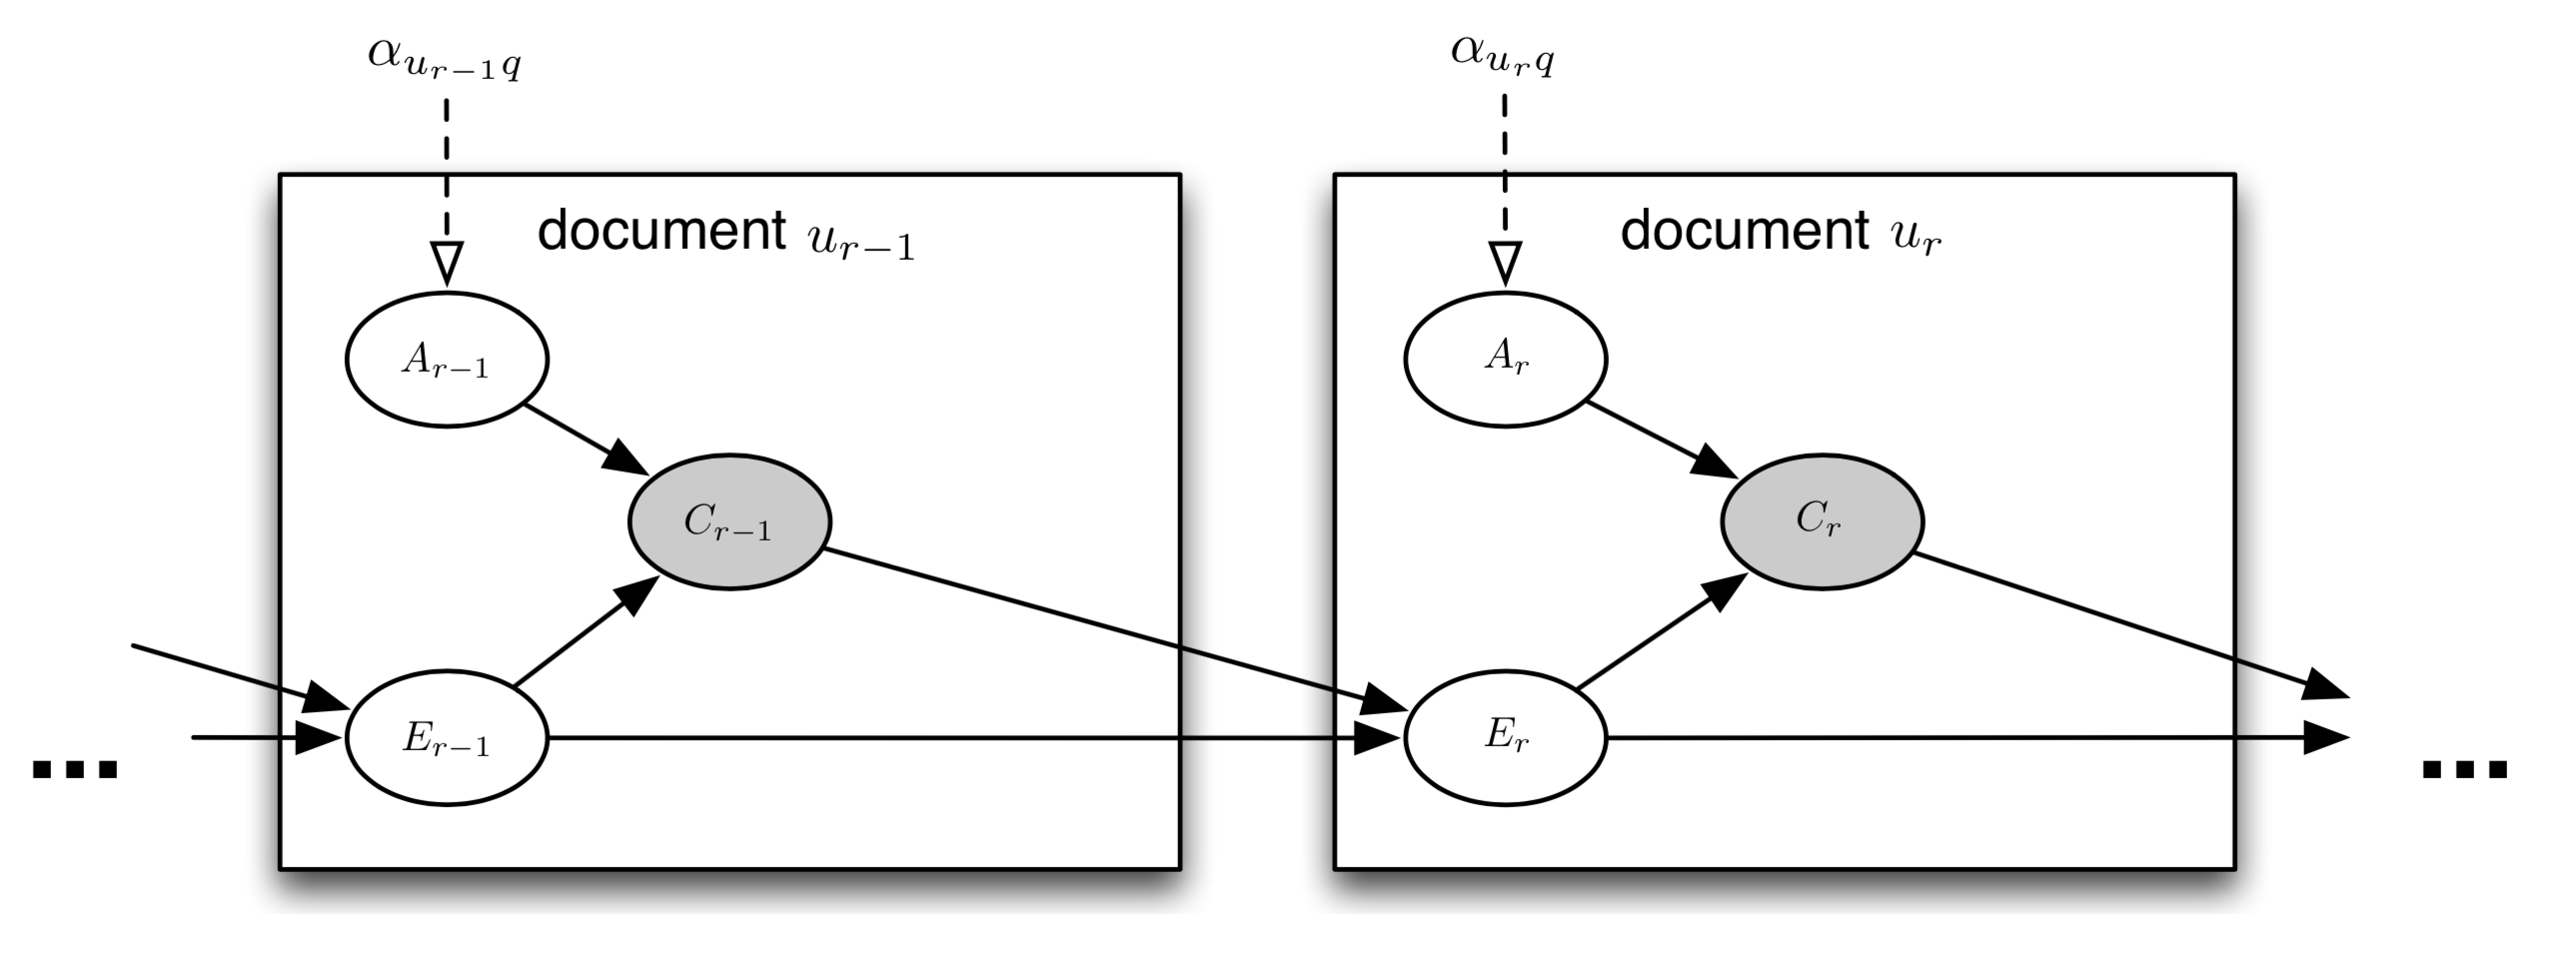
\includegraphics[width=0.5\textwidth]{figures/click_models_CM_pgm.png}
		\caption{Probabilistic graphical model of parameters for CM}
		\label{img:click_models_CM_pgm}
	\end{figure}
	\item \textit{Advantages}: Clicking on a document depends on previous decisions/documents
	\item \textit{Disadvantages}: No skips are allowed. Also, the cascade model only considers a single click $\implies$ Dynamic Bayesian Networks
\end{itemize}
\section{Introduction to Retrieval models}
\begin{itemize}
	\item Mathematical framework for defining query-document matching
\end{itemize}
\subsection{TF-IDF}
\begin{itemize}
	\item In a vector space model, documents and queries are represented in vector space
	\item Axes are mostly terms/vocabulary so that a document or query is represented by terms they contain (or their frequency)
	\item We can rank documents based on their cosine similarity with the query:
	$$\text{score}(d,q) = \frac{\vec{q} \cdot \vec{d}}{||\vec{q}||\cdot ||\vec{d}||}$$
	\item Documents can be therefore represented as non-negative vector of term weights (raw frequency in doc):
	\begin{figure}[ht]
		\centering
		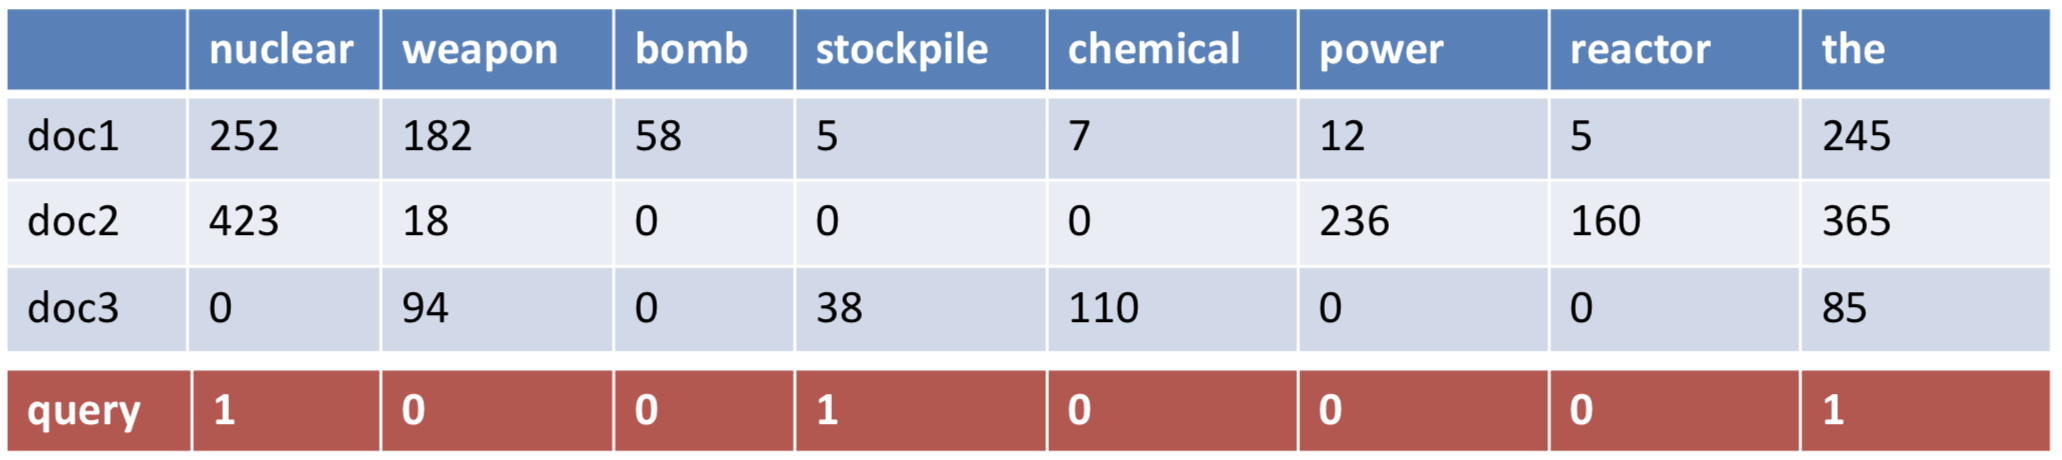
\includegraphics[width=0.5\textwidth]{figures/language_models_tf_example.png}
		\label{img:language_models_tf_example}
	\end{figure}
	\item However, the problem here is that terms with a higher frequency in documents are automatically more important, although this is not always the case (e.g. "the"). Thus, for identifying the important terms, we can report document frequency (no. of docs in which terms occurs):
	$$\text{df}(t) \coloneqq \#\left\{d:\text{tf}(t;d)>0\right\}$$
	\item We can translate document frequencies to term weights by inverting them (inverted document frequency - \textit{IDF}):
	$$\text{idf}(t) = \log \frac{n}{\text{df}(t)} = \log n - \log \text{df}(t)$$
	The log is applied to dampen the effect of IDF.
	\item Also the term frequencies should be dampened by a monotonic, sub-linear transformation as a term occurring twice as often doesn't imply that the document is also twice as important/relevant. Together, we can define the tf-idf weights as follows:
	$$\text{tf-idf}(t;d) = \log \left(1+\text{tf}(t;d)\right) \log \frac{n}{\text{df}(t)}$$
	\item Scores are normalized by euclidean distance of document. Alternatively, we could also apply tf-idf on the relative term frequencies.
\end{itemize}
\subsection{BM25}
\begin{itemize}
	\item Probabilistic retrieval framework that extends the idea of tf-idf
	\item Instead of the log, we use a different damping functions which are easier to control:
	$$w_t = \frac{(k_1 + 1)\cdot \text{tf}(d;t)}{k_1 + \text{tf}(d;t)}\cdot \text{idf}(t)$$
	\item In addition, we normalize the term frequency by the document length: $\text{tf}'(d;t) = \text{tf}(d;t) \cdot l_{avg}/l_{d}$ ($l_{avg}$ is the average document length of collection). By this we prevent copies of documents concatenated with each other being higher rated. Putting this into our original function, we get:
	$$w_t = \frac{(k_1 + 1) \cdot \text{tf}(d;t)}{k_1 \cdot (l_d / l_{avg})+ \text{tf}(d;t)}\cdot \text{idf}(t)$$
	\item However, longer documents also tend to contain more information. Thus, we introduce another parameter $b$ that controls the normalization:
	$$w_t = \frac{(k_1 + 1) \cdot \text{tf}(d;t)}{k_1 \cdot ((1-b) + b\cdot (l_d / l_{avg}))+ \text{tf}(d;t)}\cdot \text{idf}(t)$$
	\item For very long queries, we also need to consider this normalization which can be done by multiplying another term $\frac{(k_3 + 1)\cdot \text{tf}(q;t)}{k_3 \cdot \text{tf}(q;t)}$
	\item In conclusion, the BM25 score is calculated as follows:
	$$\text{BM25} = \sum\limits_{\text{unique\hspace{1mm}} t\in q} \frac{(k_1 + 1) \cdot \text{tf}(d;t)}{k_1 \cdot ((1-b) + b\cdot (l_d / l_{avg}))+ \text{tf}(d;t)} \cdot \frac{(k_3 + 1)\cdot \text{tf}(q;t)}{k_3 + \text{tf}(q;t)} \cdot \text{idf}(t)$$
	\item Parameters $k_1$, $b$ and $k_3$ are tuned. Common defaults are $k_1 = 1.5$ and $b=0.75$
	\item It is the most widely used ranking in IR but only loosely inspired by probabilistic models
\end{itemize}
\subsection{Statistical Language Models}
\begin{itemize}
	\item Statistical language models are a probability distribution over word sequences $P(w_1, ..., w_m)$ with which documents and queries can be represented (and uncertainty quantified)
	\item Thus, a language model describes the probability of e.g. $q$ being the given word sequence
	\item Documents are ranked given a query by its similarity. Therefore we can use either document likelihood, query likelihood or KL-divergence
\end{itemize}
\subsubsection{Query likelihood}
\begin{itemize}
	\item Given a document, what queries are most likely to be created for it? 
	\item We first have to ensure that the query likelihood correlates with document likelihood. Therefore, we apply the Bayes rule: $p(d|q) = \frac{p(q|d)p(d)}{p(q)}$. As $p(q)$ is equal for all documents, and we assume a uniform prior for all documents (though not always the case), we retrieve $p(d|q)\propto p(q|d)$
	\item Thus, by generating a probability distribution of possible queries for a document, we can approximate how likely a document is given a query.
	\item The scoring function is defined as follows:
	$$\text{score}(d,q) = \log \left[p(q|\theta_d)\cdot p(d)\right]$$
	where $\theta_d$ describes the document. There are mainly three modeling choices:
	\begin{enumerate}
		\item \textit{How to define the generative process $p|\theta_d$?}
		\begin{itemize}
			\item Given $\theta_d$, what is the generative process for getting $q=w_1,...,w_{|q|}$?
			\item Different distributions are possible
			\item \textit{Multiple Bernoulli} - bag of word perspective, every word in vocabulary has probability to be in query or not. The related probability is:
			$$p(q|\theta_d) = \prod\limits_{w_i \in q} p(X_i = 1 | \theta_d) \prod\limits_{w_i \not\in q} \left(1 - p\left(X_i = 1 | \theta_d\right) \right)$$
			\item \textit{Multinomial} - similar to bernoulli, but we know have a random variable for every word slot in the query and not one for every word in the vocabulary. Thus, the calculation is:
			$$p(q|\theta_d) = \prod\limits_{w_i \in q} p(w_i | \theta_d) \text{\hspace{4mm}where\hspace{4mm}} \sum\limits_{w_i \in V} p(w_i|\theta_d) = 1$$
			\item \textit{Multiple Poisson} - similar to bernoulli, but instead of presence or absence, we model the number of times we expect a word from the vocabulary to occur in the query of length $|q|$ by a Poisson distribution:
			$$p(q|\theta_d) = \prod\limits_{w_i \in V} \frac{e^{-\lambda_i |q|} (\lambda_i |q|)^{\text{tf}(w_i;d)}}{\text{tf}(w_i;d)!}$$
		\end{itemize}
		\item \textit{How to estimate $\theta_d$ based on document $d$?}
		\begin{itemize}
			\item To estimate $\theta_d$ we perform MLE: $\hat{\theta}_d = \arg \max_{\theta_d} p(d|\theta_d)$
			\item In case of a multinomial distribution, we would get:
			$$p(d|\theta_d) = \prod\limits_{w_i \in V} p(w_i | \theta_d)^{\text{tf}(w_i;d)} \implies \log p(d|\theta_d) = \sum\limits_{w_i \in V} \text{tf}(w_i;d) \log p(w_i | \theta_d)$$
			\item Note that this is a constrained optimization problem with $\sum\limits_{w_i \in V} p(w_i|\theta_d) = 1$.
			\item By using lagrangian multiplier, we get $p_{MLE}(w_i|d) = \frac{\text{tf}(w_i;d)}{|d|}$
		\end{itemize}
		\item \textit{How to compute prior $p(d)$?}
		\begin{itemize}
			\item The prior takes everything into account which is independent of a query.
			\item This can include number of clicks, credibility, ...
		\end{itemize}
	\end{enumerate}
\end{itemize}
\subsubsection{Smoothing}
\begin{itemize}
	\item How to deal with unseen words which have a probability of 0.
	\item First, we assume a multinomial distribution again with the optimal parameters of $p(w_i|\theta_d) = \frac{\text{tf}(w_i;d)}{|d|}$
	\item \textbf{Adaptive smoothing}: add a small extra count to every word:
	$$p(w_i|\theta_d) = \frac{\text{tf}(w_i;d) + \epsilon}{|d| + \epsilon |V|}$$
	In case of $\epsilon=0$, we fall back to ML estimation. $\epsilon=1$ is called Laplace smoothing.
	\item \textbf{Jelinek-Mercer smoothing}: linearly interpolate with "background" knowledge so that rare words also have smaller additives:
	$$p_{\lambda}(w_i|\theta_d) = \lambda \frac{\text{tf}(w_i;d)}{|d|} + (1 - \lambda) \frac{\text{tf}(w_i;C)}{|C|}$$
	The context $C$ is approximated by the concatenation of all documents.
	\item \textbf{Dirichlet prior smoothing}: we assume that before seeing the document, we have a prior belief over all words $p(\theta_d)$. We use the posterior which gets narrower the more words we see and therefore the more certain we are about the document distribution.
	\begin{itemize}
		\item Maximum A Posteriori estimate by $\hat{\theta}_d = \arg\max_{\theta_d} p(\theta_d|d) = \arg\max_{\theta_d} p(d|\theta_d) p(\theta_d)$
		\item Prior distribution $p_i\sim \text{Dir}(\alpha) \implies p(\theta_d) = \prod\limits_{w \in V} p(w|\theta_d)^{\alpha_w - 1}$
		\item With a multinomial likelihood, we get:
		$$p(\theta_d | d) \propto \prod\limits_{w \in V} p(w|\theta_d)^{\text{tf}(w;d)} \prod\limits_{w \in V} p(w|\theta_d)^{\alpha_w - 1} = \prod\limits_{w \in V} p(w|\theta_d)^{\text{tf}(w;d) + \alpha_w - 1}$$
		\item Thus, our new MAP solution is:
		$$p(w|\theta_d) = \frac{\text{tf}(w;d) + \alpha_w - 1}{|d| + \sum_{w\in V}\alpha_w - |V|}$$
		\item For $\alpha_w = 1$, we get MLE estimation, and $\alpha_w = 2$ represents Laplace smoothing.
		\item We can also rewrite the smoothing similar to Jelinek-Mercer smoothing:
		$$p(w|\theta_d) = \frac{|d|}{|d|+ \mu}\frac{\text{tf}(w;d)}{|d|} + \frac{\mu}{\mu + |d|}p(w|C)$$
		where $\mu$ is the parameter depending on $\alpha_w$. Thus, we interpolate with the background knowledge while taking the document length into account.
	\end{itemize}
	\item Next to Dirichlet prior smoothing, we can also use other distributions (for example a beta prior with multiple Bernoulli) which lead to slightly different smoothing functions. For example, with the beta prior, we get for a variable $\alpha_w$ and $\beta_w$ (without constraints!):
	$$p(w|\theta_d) = \frac{\text{tf}(w;d) + \alpha_w - 1}{\alpha_w + \beta_w - 1}$$
\end{itemize}
\subsubsection{Positional Language Models}
\begin{itemize}
	\item There are variants of basic language models capturing term dependencies
	\item Instead of having one language model representing the whole document, Positional Language Models define a LM for every word position
	\item Thus we capture (small) "fuzzy" passages with which we can match our query
	\item A term at each position can propagate its occurrence to close positions in word windows
	\begin{itemize}
		\item Example sentence: \texttt{the black hat is not}...
		\item With a equally weighted word window of one, we would retrieve the following language model (MLE params) for the position of word "\texttt{black}": $p(\texttt{black}|\theta_p) = 1/3, \hspace{2mm} p(\texttt{the}|\theta_p) = 1/3, \hspace{2mm} p(\texttt{hat}|\theta_p) = 1/3$
	\end{itemize}
	\item We can weight the occurrences of every word based on the distance to the "root" of the language model (also called kernel):
	\begin{figure}[ht]
		\centering
		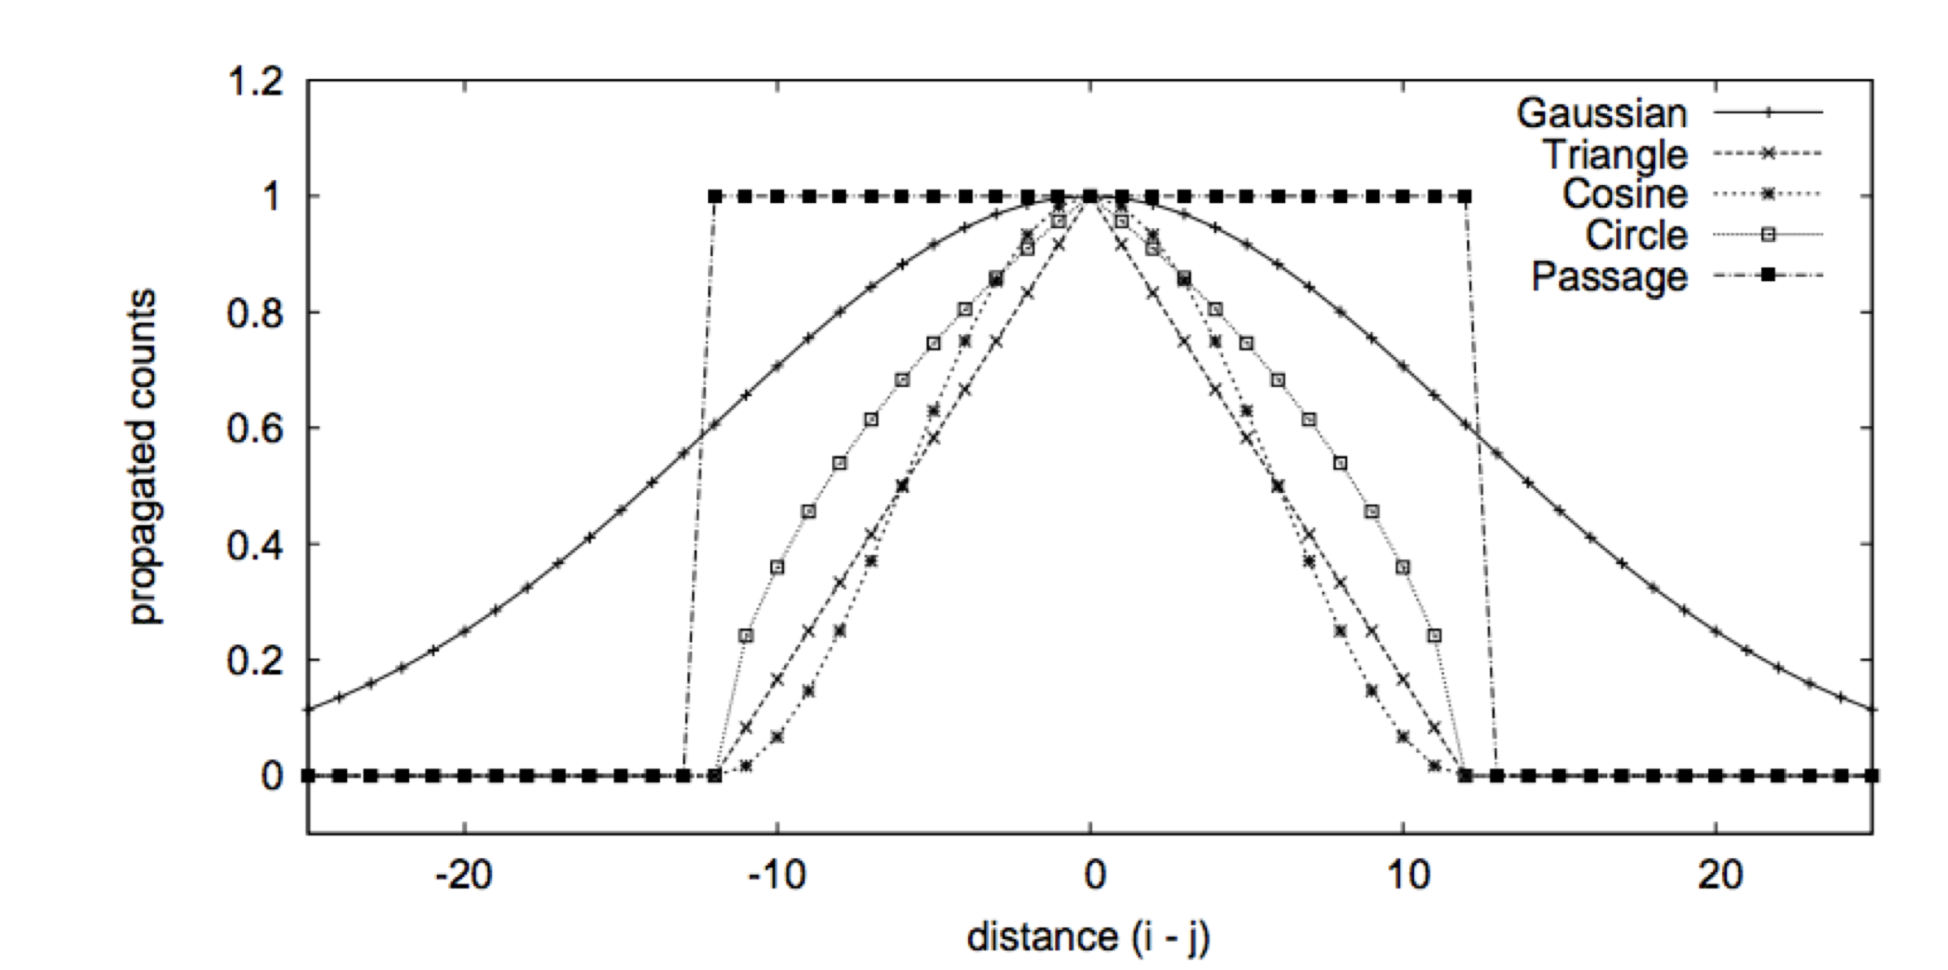
\includegraphics[width=0.4\textwidth]{figures/language_models_positional.png}
		\label{img:language_models_positional}
	\end{figure}
	\item In general, the term frequency of a word for a LM at position $j$ with kernel $k$ is determined as follows:
	$$\text{tf'}(w,j;d) = \sum\limits_{i=1}^{|d|} \text{tf}(w,i;d) \cdot k(i,j) $$
	\item The language model at every position is given by the corresponding MLE estimation:
	$$p(w|d,j) = \frac{\text{tf'}(w,j;d)}{\sum_{w'\in V} \text{tf'}(w',j;d)}$$
	\item Documents can now be scored by either their best matching language model with the query, or the average of the top-$k$ models
\end{itemize}
\section{Semantic matching}
\begin{itemize}
	\item \textit{Vocabulary gap}: query and document might use different lexical representation for the same entity $\implies$ resolve by semantic matching
	\item Represent query and document by their meaning, not lexical/word level
	\item This will help to identify synonyms and/or semantic relatedness for computing similarity
	\item To get such a representation, one idea is to apply dimensionality reduction. This relies on the assumption that the dimension of the data is actually lower than i.e. vocabulary size
	\item Similar data in terms of semantic will be (hopefully) similar in reduced dimensions as well
\end{itemize}
\subsection{Latent Semantic Indexing}
\begin{itemize}
	\item We represent all documents and queries in a term-document matrix:
	$$X = \left[\begin{array}{cccc}
	| & | &  & | \\
	x_1 & x_2 & \dots & x_m \\
	| & | &  & | 
	\end{array}\right]$$
	where $m$ rows represent the documents, and $n$ rows the terms. A single cell in the matrix $X$ specifies the term frequency $\text{tf}(w;d)$. Note that we would also add the queries in $X$ as documents.
	\item On this matrix, we apply Singular Value Decomposition (SVD) so that $X_{n\times m} = U_{n \times r} \Sigma_{r\times r} V_{m\times r}^T$
	\begin{itemize}
		\item $\bm{U}_{n \times r}$ represents the word/term embedding along rows (one word per row). The columns are the "semantic" dimensions that e.g. represent topics/hidden lower-dimensional space. 
		\item $\bm{V}_{m \times r}$ similarly represents the embedding of documents (one doc per row, but is transposed in calculation). 
		\item $\bm{\Sigma}_{r \times r}$ is a square, diagonal matrix. The magnitude of a singular value represents the importance of the corresponding latent dimension in the collection/data. It is always sorted from the highest value in first place to lowest value in last place.
	\end{itemize}
	\begin{figure}[ht]
		\centering
		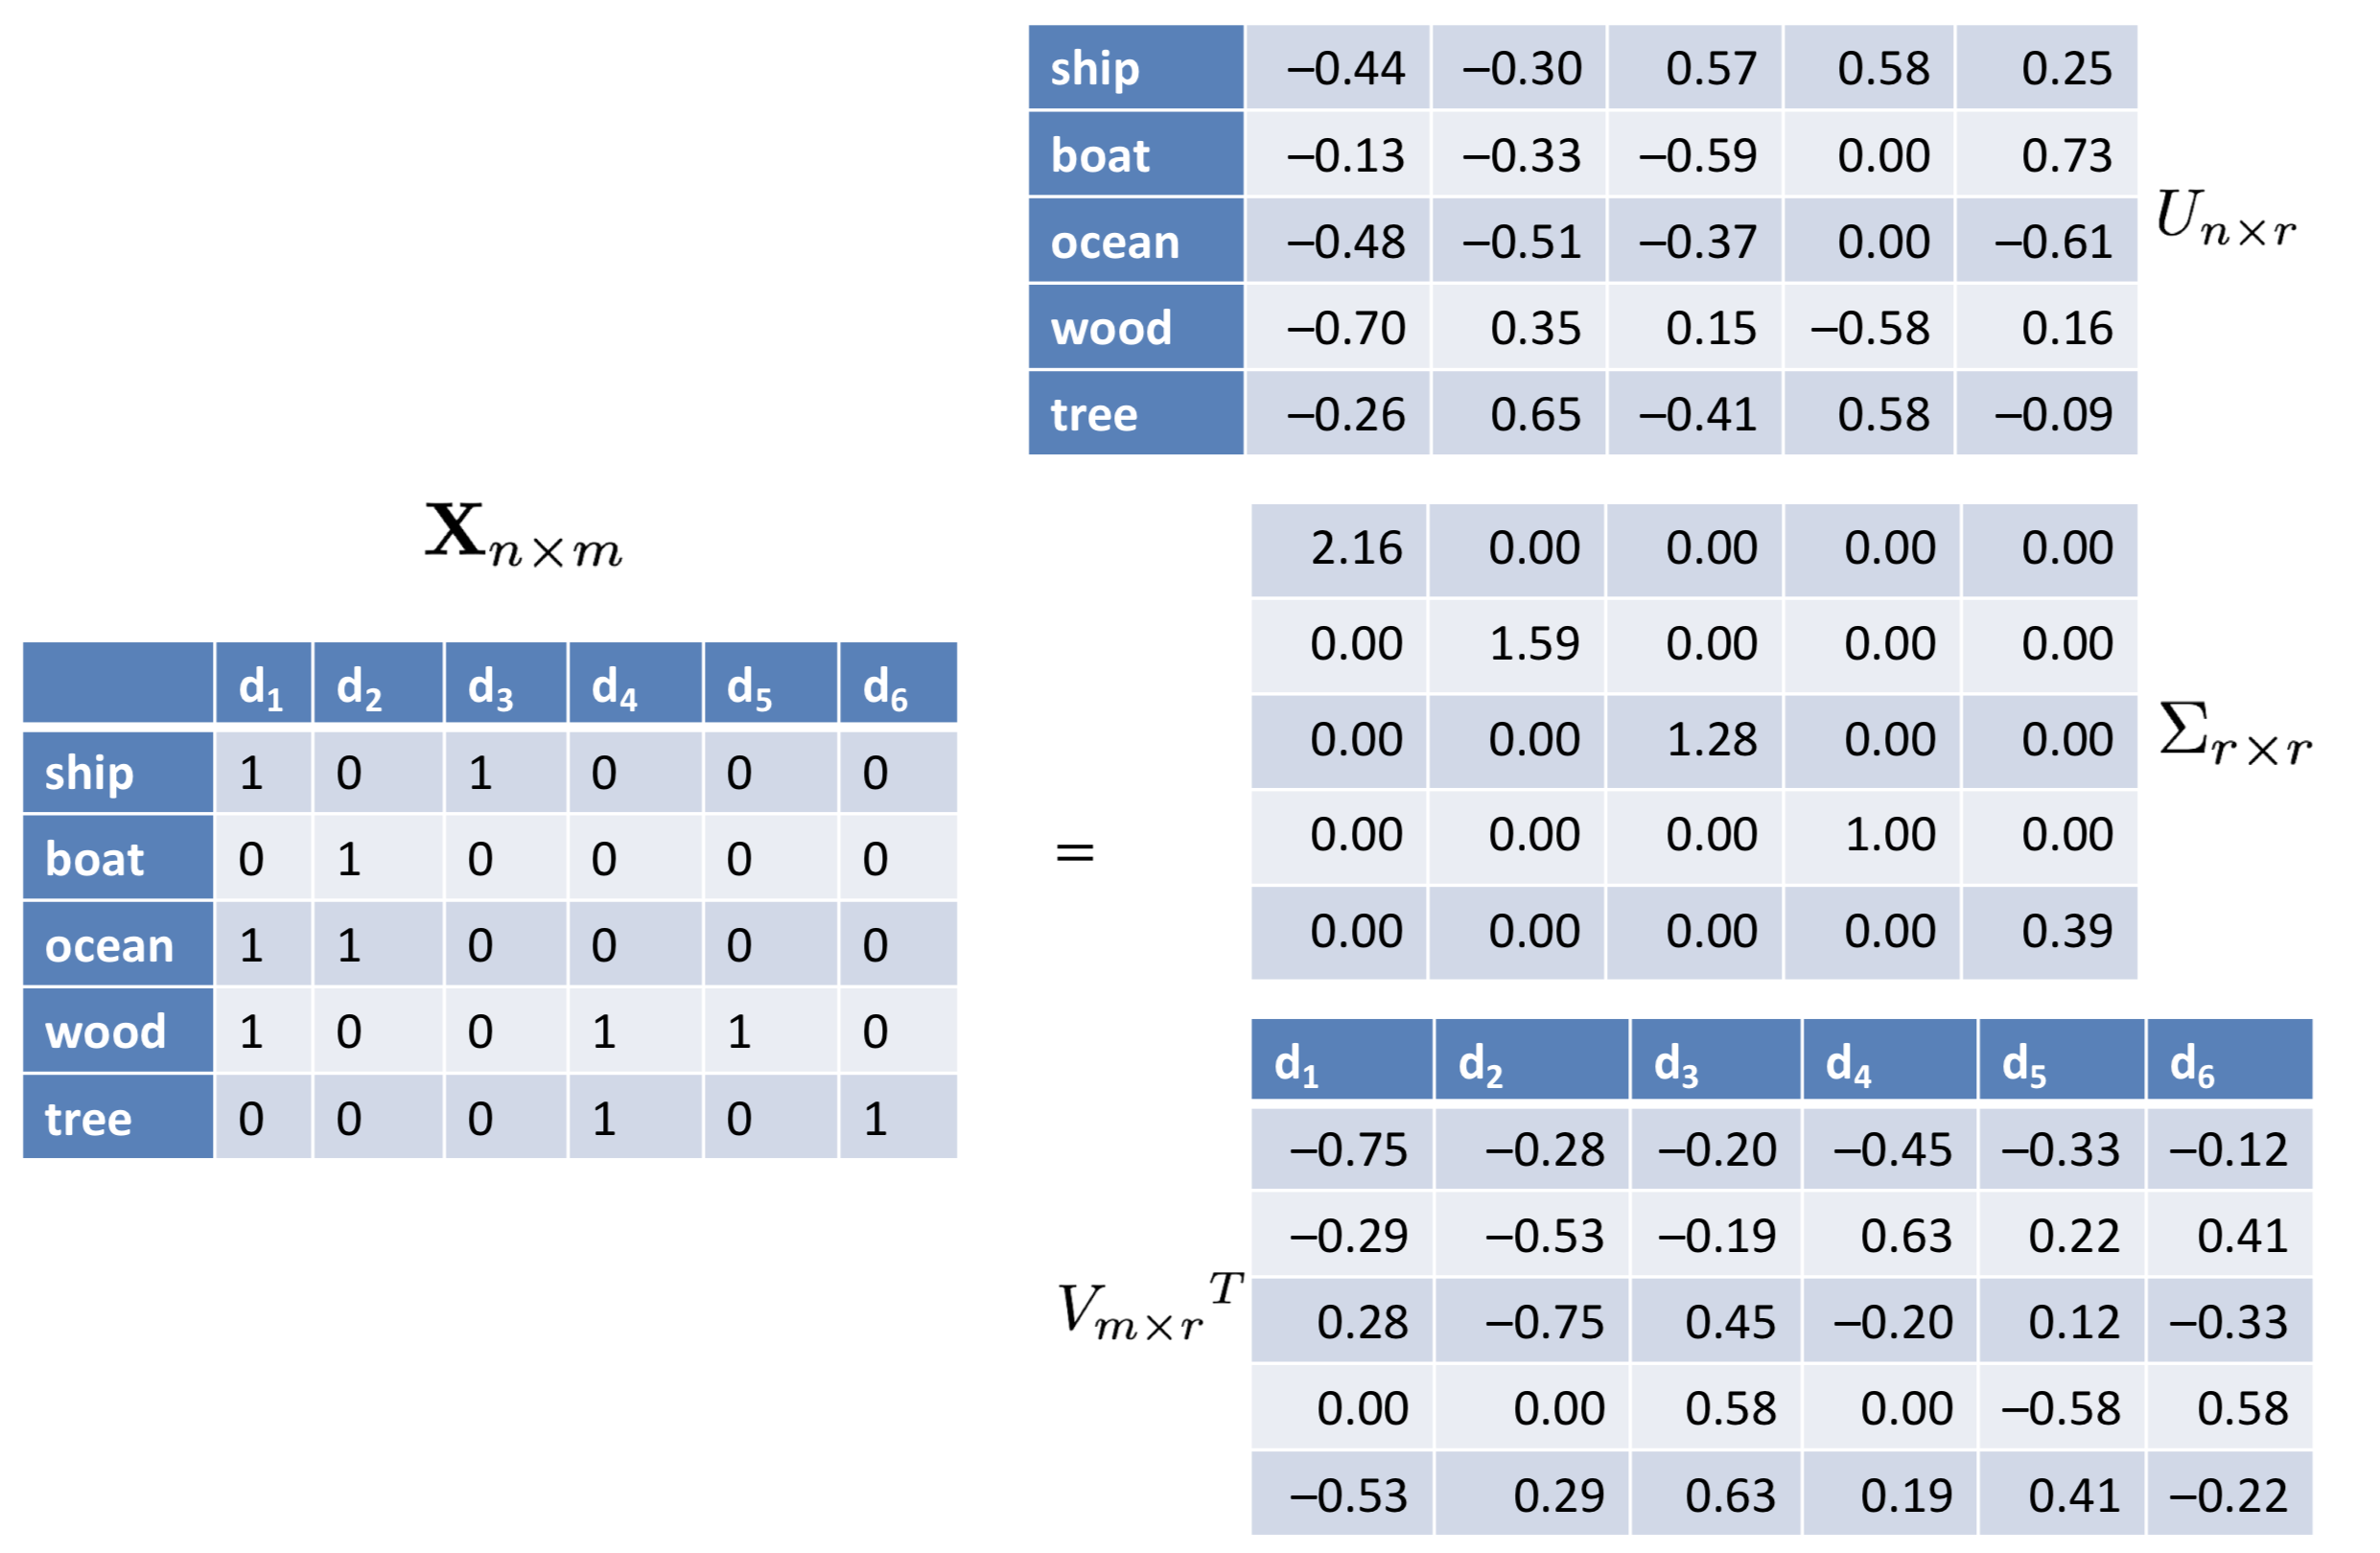
\includegraphics[width=0.5\textwidth]{figures/semantic_matching_SVD_example.png}
		\caption{Example of SVD for 6 documents and 5 terms}
		\label{img:semantic_matching_SVD_example}
	\end{figure}
	\item To reduce dimensions to $k$, we simply drop those with the lowest values in $\Sigma$. These dimensions may be noise and make things dissimilar when they actually are on topic level. $k$ is hyperparameter.
	\item In case of Figure~\ref{img:semantic_matching_SVD_example} with $k=2$, we would drop the last three dimensions. This leads to our new embeddings $X'$ for the documents. The resulting matrices would look like as in Figure~\ref{img:semantic_matching_SVD_example_2}.
	\begin{figure}[ht]
		\centering
		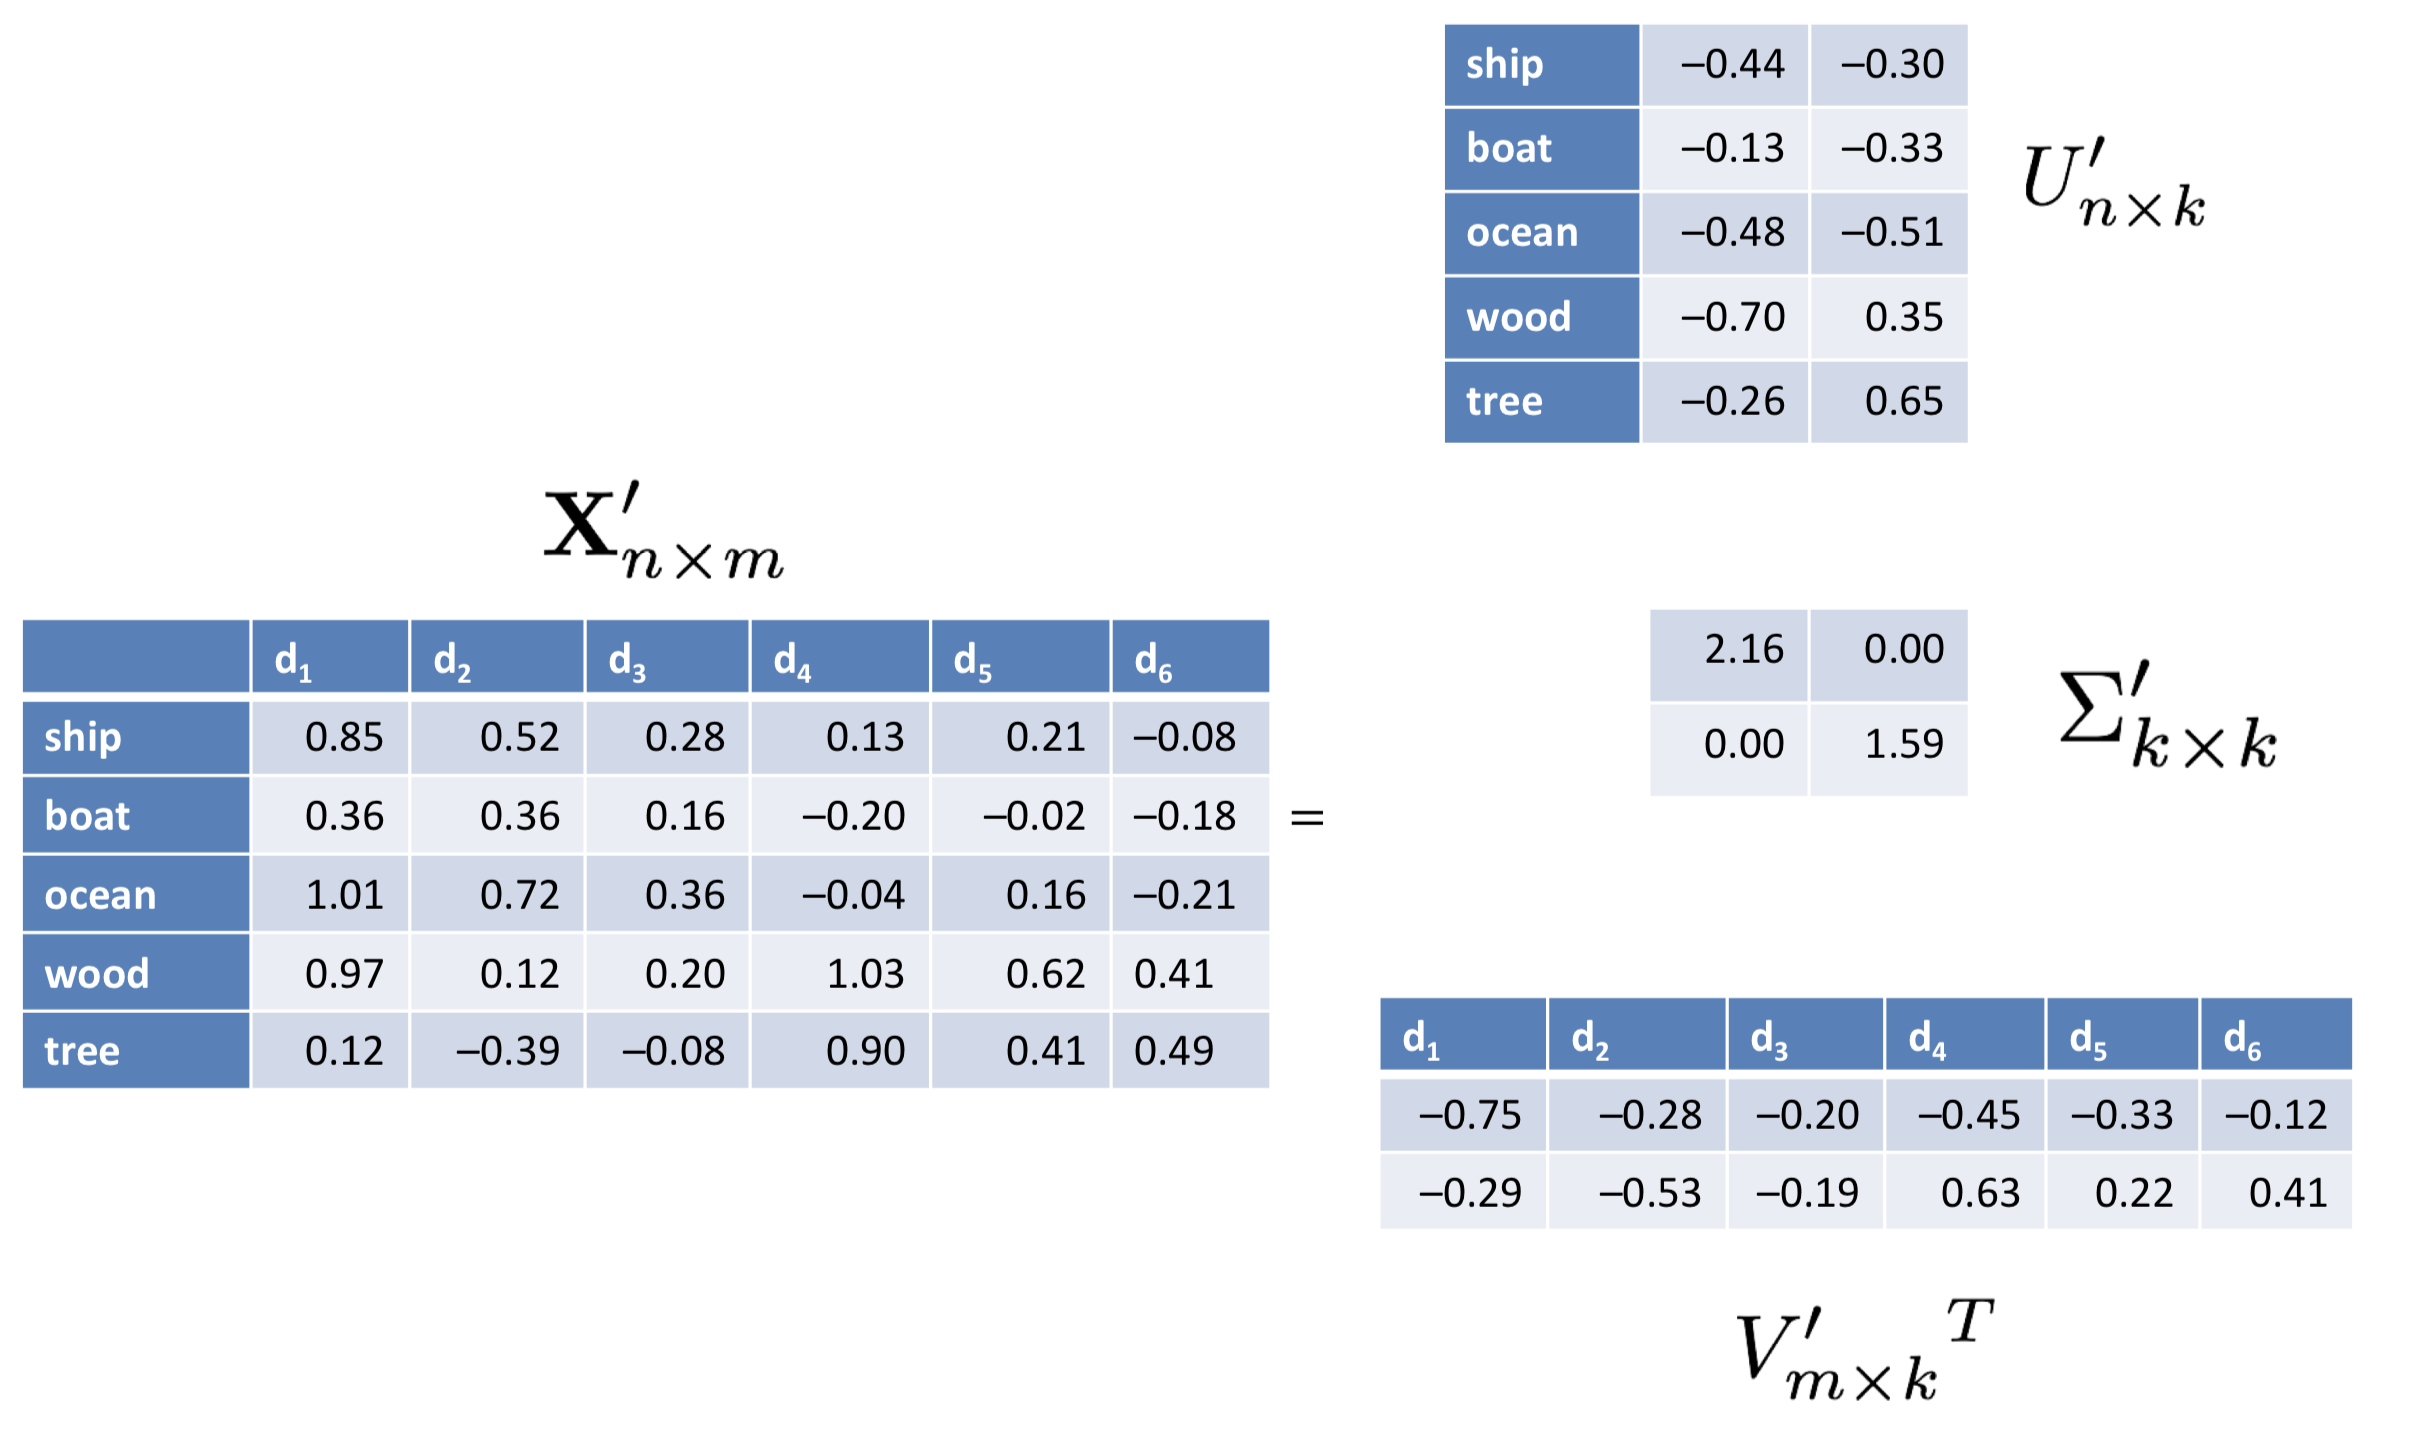
\includegraphics[width=0.5\textwidth]{figures/semantic_matching_SVD_example_2.png}
		\caption{Reduced dimensions by $k=2$ for 6 documents and 5 terms}
		\label{img:semantic_matching_SVD_example_2}
	\end{figure}
	\item The similarity between documents/queries can be calculated by cosine similarity (dot product) between their new embeddings in $X'$. Furthermore, we can also compute the similarity between terms by using the rows.
	\item Choice of $k$:
	\begin{itemize}
		\item The choice of $k$ is critical in IR. The ideal value of $k$ would be large enough to fit all the real structure in the data, but small enough to compress/group terms together that are very similar (less noise).
		\item Typically, different values of $k$ are tested and compared by their performance. For example, a high precision but low recall suggests a poor generalization of the model. Therefore, we should decrease $k$ in this case.
	\end{itemize}
	\item LSI addresses synonymy by mapping similar words in the same dimensions. The cost of such a mapping is lower than for unrelated words as they occur similar/same documents. 
	\item \textbf{Strengths} of LSI
	\begin{itemize}
		\item Using $X'$ instead of $X$ show performance increase as we filter out the noise
		\item $X'$ represents the best approximation of $X$ with a matrix of rank $k$: $X' = \argmin\limits_{X':\text{rank}(X')=k} ||X-X'||$
		\item Is mostly combined with lexical methods like BM25 to not lose "obvious" matches
	\end{itemize}
	\item \textbf{Weaknesses} of LSI
	\begin{itemize}
		\item A huge storage is required as the matrices $U$ and $V$ are dense (less zeros)
		\item Representations are not interpretable, and it is not guaranteed that hidden dimensions represent topics
		\item $k$ is often not easy to determine and requires multiple tests
		\item SVD assumes orthogonal dimensions on which the variance is maximum which is not always the case
		\item The model is not generative or probabilistic, which makes it hard to extend collection by new documents/queries (worst case: redo whole SVD)
	\end{itemize}
	\item One alternative is Non-negative Matrix Factorization which leads to smaller, positive matrices (but doesn't solve the other problems)
\end{itemize}
\subsection{Probabilistic Latent Semantic Indexing}
\begin{itemize}
	\item (Pseudo-)generative model with which we try to detect key topics in the collection in an unsupervised fashion. The model describes how we would generate docs for certain topics
	\item Every topic has its own language model/distribution over words in vocabulary in a unigram/bag-of-word style: $p(w|z=1), p(w|z=2),...$ where $z$ is the variable representing the topics. 
	\item A document is represented by the distribution of these topics in the document. Generating a document would require to first sample a topic based on the topic distribution of the document, and then generating a word based on the language model of the topic. The order of the words is not taken into account. An example is shown in Figure~\ref{img:semantic_matching_PLSI_example}.
	\begin{figure}[ht]
		\centering
		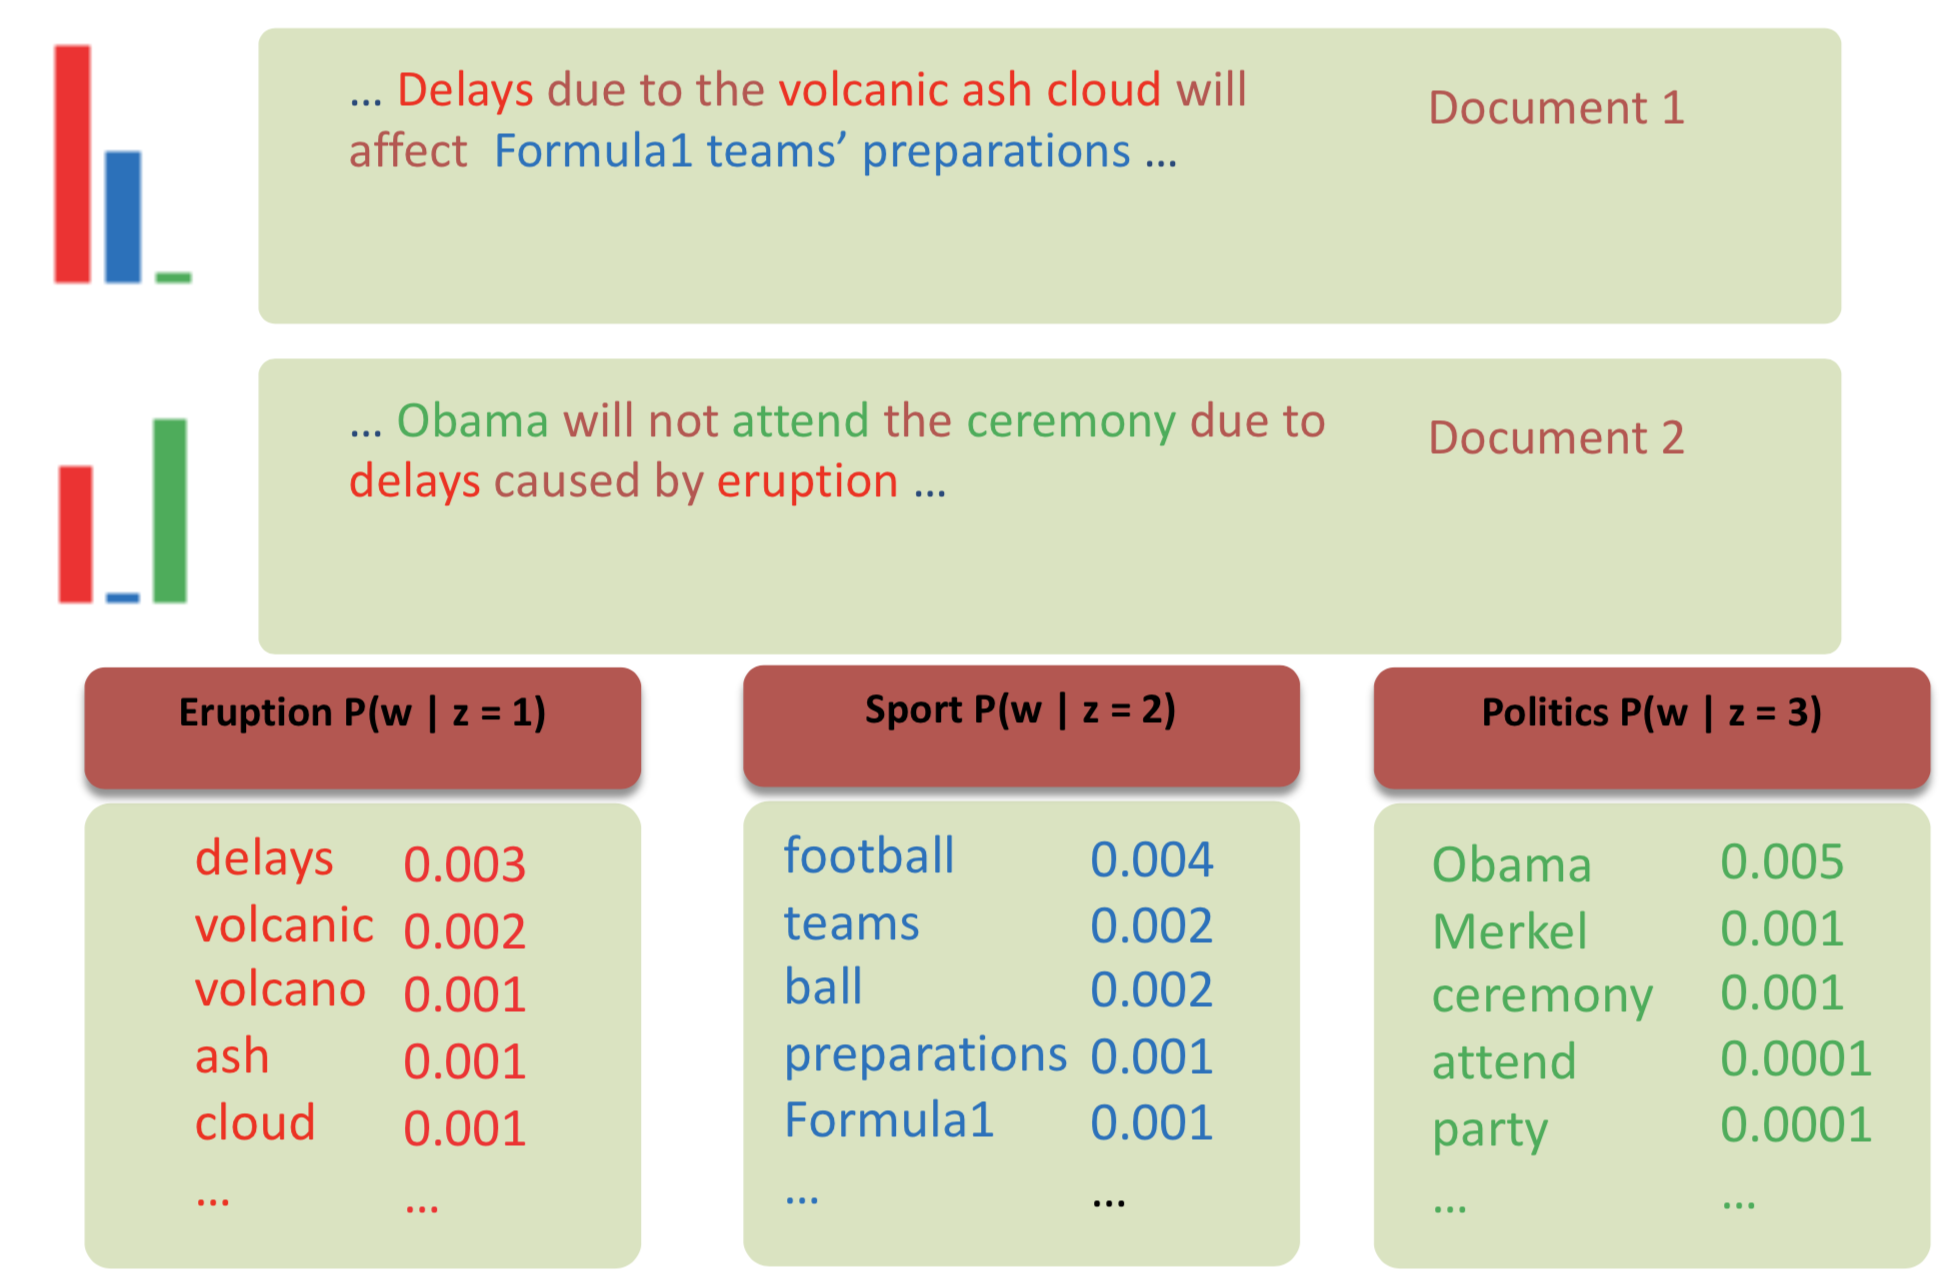
\includegraphics[width=0.5\textwidth]{figures/semantic_matching_PLSI_example.png}
		\caption{Example of document representation in PLSI}
		\label{img:semantic_matching_PLSI_example}
	\end{figure}
	\item For semantic matching, we calculate the cosine similarity between the topic distributions of the query and the document.
	\item PSLA can have problems with stop words (common words that occur in every document frequently like "the" or "and"). To prevent that, we summarize all stop words in a separate background topic model which is equally shared by all docs. Before generating a word, we toss a biased coin to decide whether to retrieve a word from the background or standard topic model. Note that in matching, these stop words are masked out by that
\end{itemize}
\subsubsection{Retrieving distributions}
\begin{itemize}
	\item Input: collection of $N$ documents, number of topics $K$
	\item Output:
	\begin{itemize}
		\item Distributions over words $\phi_{(z,w)} = p(w|z)$ for $z\in \left\{1,...,K\right\}$ with $\sum_{w\in V} p(w|z) = 1$
		\item Distributions over topics in all documents: $\theta_{d,z} = p(z|d)$ for every $d$, with $\sum_{z=1}^{K} p(z|d) = 1$
	\end{itemize} 
	\item We try to solve problem by MLE. The probability of $w$ appearing at position $i$ in the document $d$ is:
	$$p(d_i = w | \Phi, \theta_d) = \sum\limits_{z=1}^{K} \phi_{(z,w)} \theta_{d,z}$$
	The joint likelihood of the entire dataset is:
	$$p(W|\Phi, \Theta) = \prod\limits_{d\in D}\prod\limits_{w\in V}\left(\sum\limits_{z=1}^{K} \phi_{(z,w)} \theta_{d,z}\right)^{\text{tf}(w;d)} $$
	\item Taking the two constraints into account, we get an optimization problem which we can solve by the EM algorithm. For that, we assume that we know from which topic a word was generated at position $i$ in the document by $R_{d_i}$:
	$$p(W|R,\Phi,\Theta) = \prod\limits_{d\in D}\prod\limits_{i=1}^{N_i}\sum\limits_{z=1}^{K} R_{(d_i,z)} \left(\phi_{(z,w)} \theta_{d,z}\right)$$
	\item For the EM algorithm, we would update $R_{d_i}$ during the expectation step by $R_{d_i} = \frac{\phi_{(z,w_i)\theta_{(d,z)}}}{\sum_{z=1}^{K} \phi_{(z,w_i)\theta_{(d,z)}}}$. The maximization step consists of updating $\Theta$ and $\Phi$: $\theta_{(d,z)} = \frac{\sum_{d_i} R_{(d_i,z)}}{|d|}$, $\phi_{(z,w)} = \frac{\sum_{d \in D} n(d,w) R_{(w,z)}}{\sum_{w' \in V} \sum_{d \in D} n(d,w')R_{(w',z)}}$
	\item PLSA is able to learn topics with their corresponding word distributions. However, there are still some drawbacks:
	\begin{itemize}
		\item It is still not a fully generative model. After running PSLA, we have topic distribution for documents we initially had, but we cannot extend it to new documents (or only hardly with heuristics)
		\item Prone to overfitting
	\end{itemize}
\end{itemize}
\subsubsection{Latent Dirichlet Allocation (LDA)}
\begin{itemize}
	\item Takes PLSA but makes it a generative model with Dirichlet prior. Can also be seen as a Bayesian treatment of PLSA
	\item Instead of probabilities for every document, we now simply define two hyperparameters $\alpha$ and $\beta$
	\item For every topic $z=1,...,K$, we draw a word distribution $\phi_z \sim \text{Dir}(\beta)$. Thus, $\beta$ determines how words are distributed per topic
	\item For each document $d$, we sample a topic distribution $\theta_d \sim \text{Dir}(\alpha)$. The alpha therefore controls the mixture of topics for any given document.
	\item The words in the documents are then sampled by the probabilities $\phi_z$ and $\theta_d$. Note that this is a fully generative model as we can generate as many new documents as we need.
\end{itemize}
\subsubsection{Graphical Models and Probabilistic Topic Models}
\begin{itemize}
	\item We can represent every probabilistic topic model as graphical model which abstracts the conditional independence relationships
	\item For example, Figure~\ref{img:semantic_matching_graphical_models_LDA} visualizes the graphical model of the Latent Dirichlet Allocation
	\begin{figure}[ht]
		\centering
		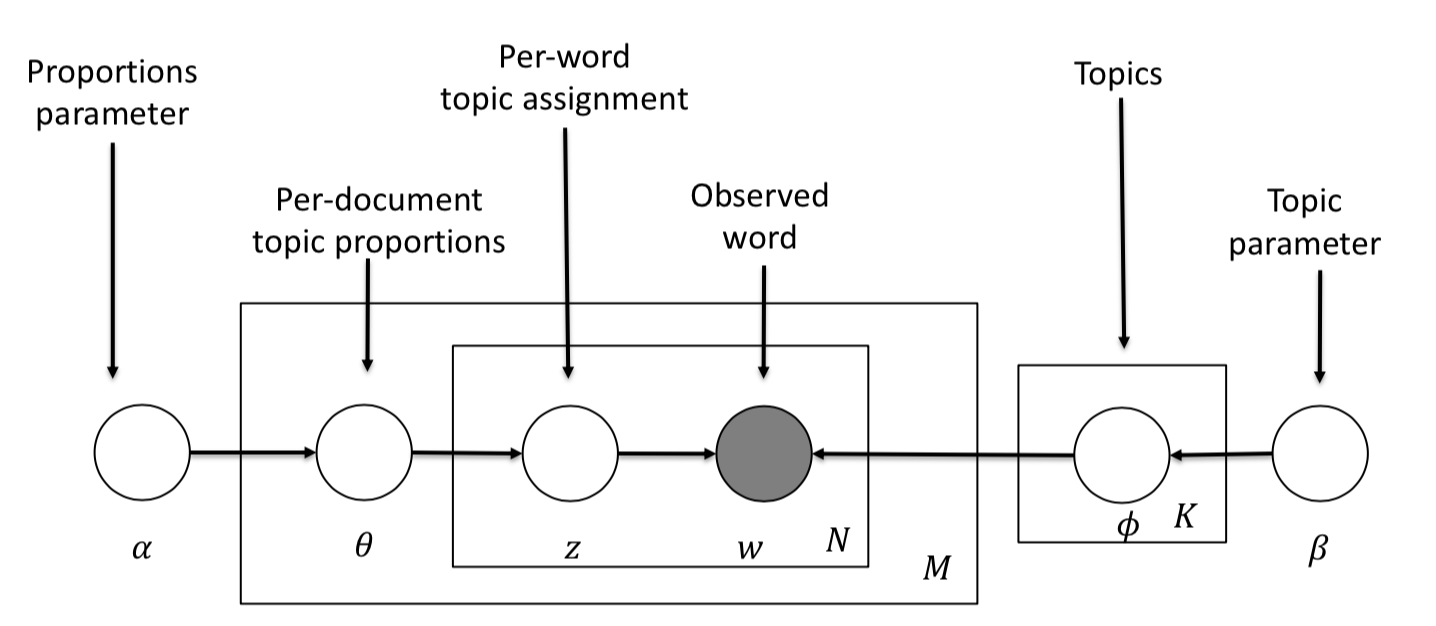
\includegraphics[width=0.5\textwidth]{figures/semantic_matching_graphical_models_LDA.png}
		\caption{Graphical model of LDA}
		\label{img:semantic_matching_graphical_models_LDA}
	\end{figure}
	\item In this diagrams, it is easier to show extensions. For instance, Figure~\ref{img:semantic_matching_graphical_models_author_model} visualizes the Author-Topic model where we add an observed variable of the author of a document. This observation affects the probability distributions over words for each topic in a document 
	\begin{figure}[ht]
		\centering
		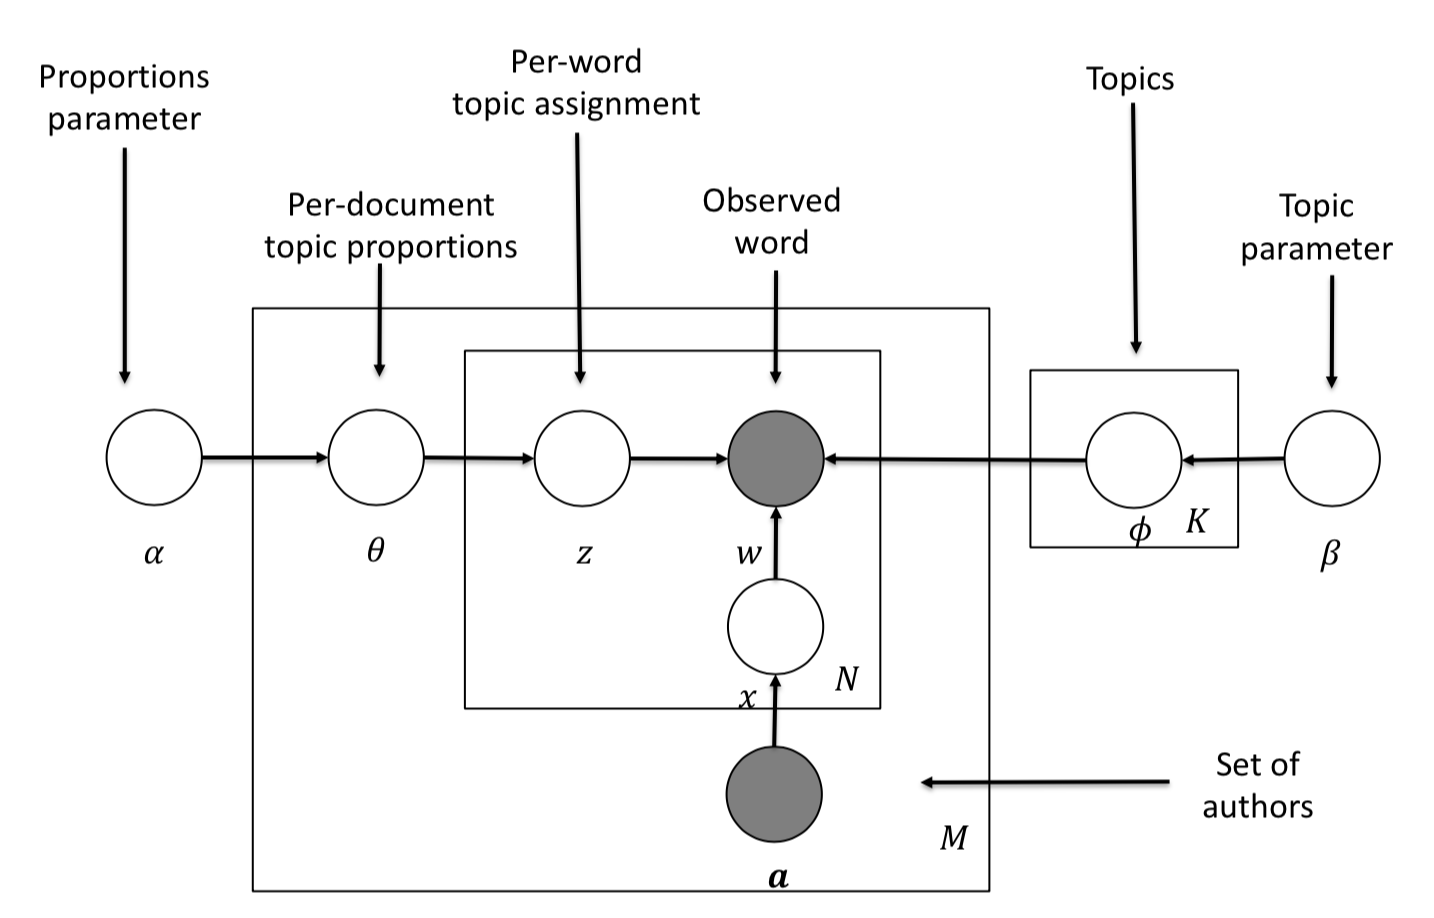
\includegraphics[width=0.5\textwidth]{figures/semantic_matching_graphical_models_author_model.png}
		\caption{Graphical model of the Author-topic model}
		\label{img:semantic_matching_graphical_models_author_model}
	\end{figure}
	% semantic_matching_graphical_models_author_model.png
\end{itemize}
\subsection{Probabilistic Topic Models in IR}
\begin{enumerate}
	\item \textbf{Topic matching}
	\begin{itemize}
		\item Represent document by $p(z|d)$ and query by $p(z|q)$
		\item Take the KL divergence or similar measure to find score/similarity between the distributions
		\item But: query is very short so that topic model is harder to infer without having too much noise
	\end{itemize}
	\item \textbf{Smoothing}
	\begin{itemize}
		\item Smooth probabilities according to the topics in the document:
		\begin{equation*}
			\begin{split}
				p(w|d) & = \lambda p_{\mu}(w|d) + (1 - \lambda) p_{\text{tm}}(w|d)\\
				& = \lambda p_{\mu}(w|d) + (1 - \lambda) \left(\sum\limits_{z=1}^{K} p(w|z) p(z|d)\right)
			\end{split}
		\end{equation*}
		\item Thus we apply Jelinek-Mercer smoothing where the context is replaced by the topic word distributions of the document
	\end{itemize}
	\item \textbf{Query expansion}
	\begin{itemize}
		\item We can build an own language model for a given query by using the word distributions of the topics:
		$$p_{\text{tm}}(w|q) = \sum\limits_{z=1}^{K} p(w|z) p(z|q)$$
	\end{itemize}
\end{enumerate}
\section{Neural Retrieval Models}
\subsection{Distributed Word Representations}
\begin{itemize}
	\item Latent, dense vector representation to model semantic similarity/relations
	
\end{itemize}
\subsubsection{Skip-gram}
\begin{itemize}
	\item \textbf{Skip gram}: learn to predict neighboring words in a small context window
	\item Model probability by similarity between word and context vectors (two matrices):
	$$p(w_k|w_j) = \frac{\exp\left(c_k \cdot v_j\right)}{\sum_{i\in|V|}} \exp\left(c_i \cdot v_j\right)$$
	\item Denominator can be computationally expensive if vocabulary is quite large. Thus, we can approximate it by taking just a few negative examples $\implies$ negative sampling
	\item Overall, skip gram will learn two representations for each word (context $C$ and target words $V$) from which me most likely only use $V$ (visualized in Figure~\ref{img:neural_ir_skip_gram})
	\begin{figure}[ht]
		\centering
		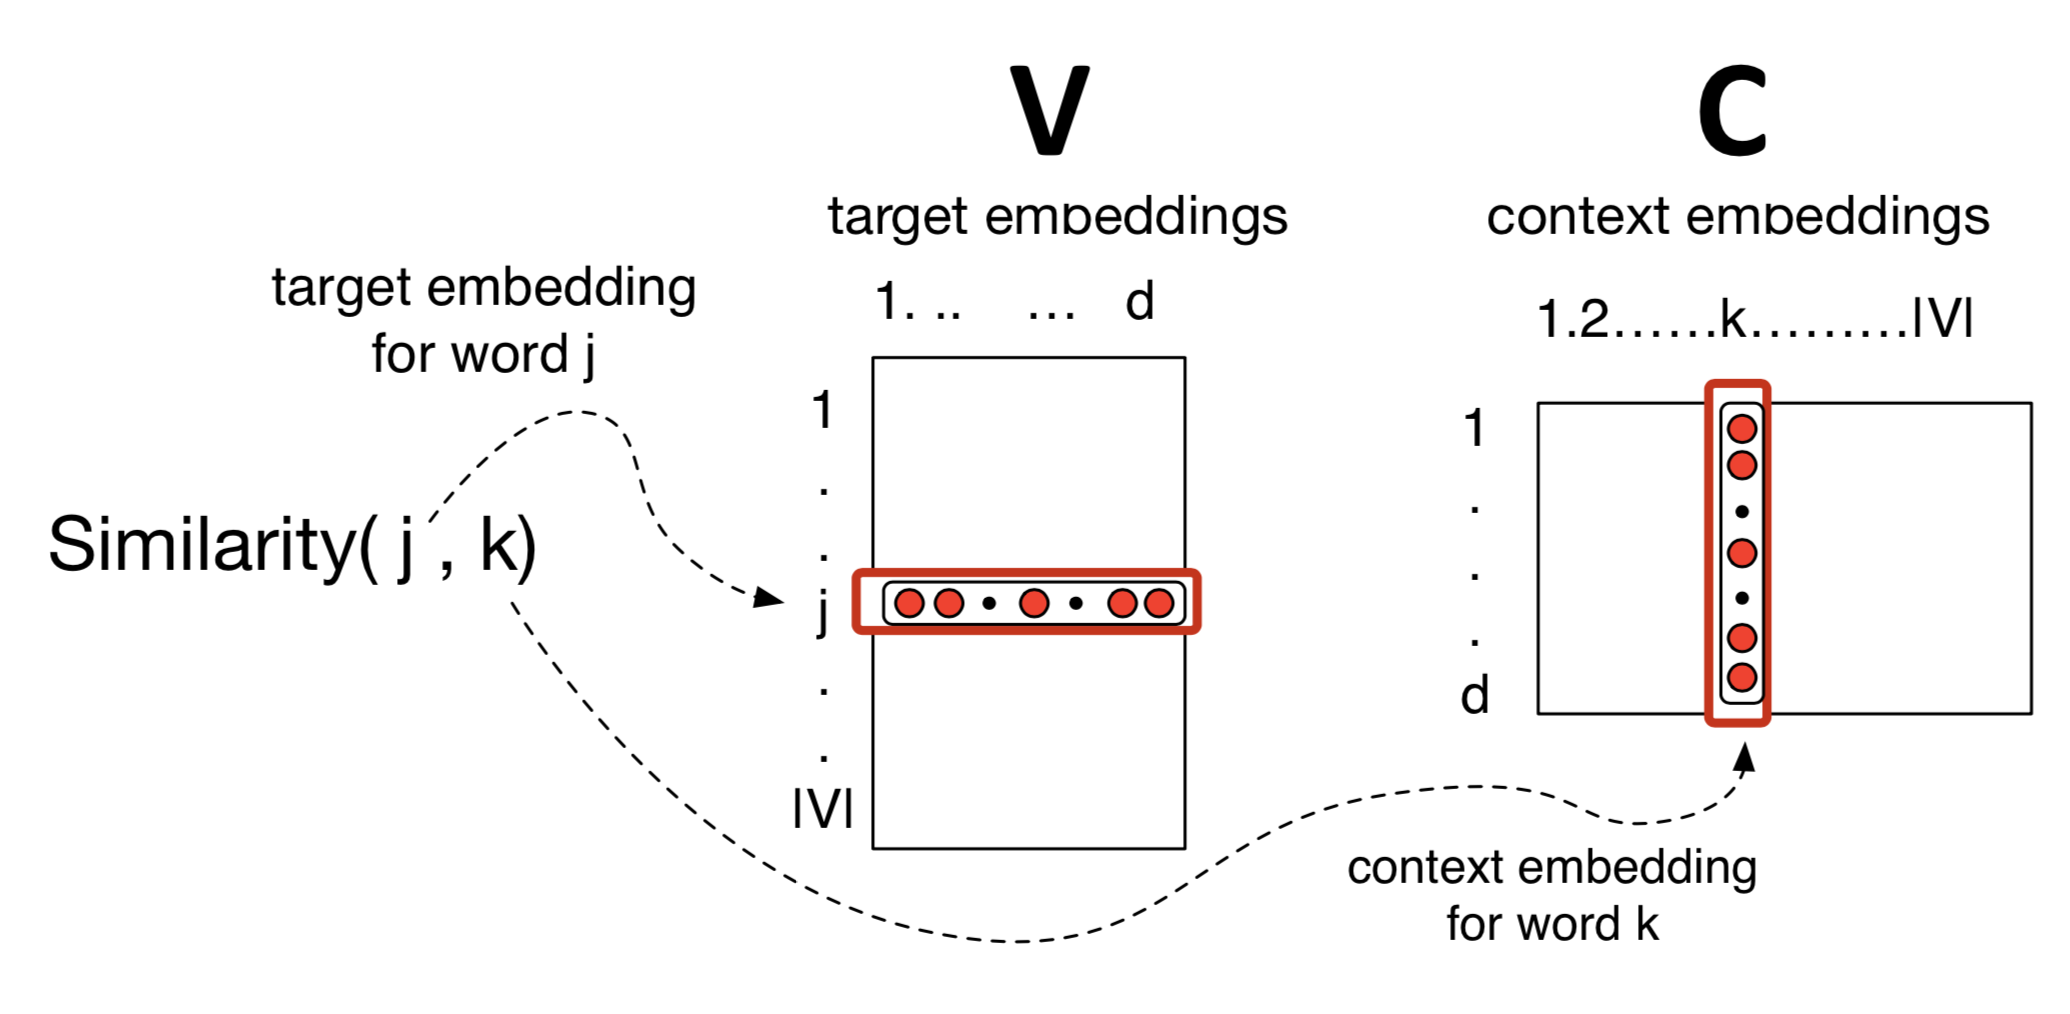
\includegraphics[width=0.4\textwidth]{figures/neural_ir_skip_gram.png}
		\caption{Visualization of skip gram method for learning word representations}
		\label{img:neural_ir_skip_gram}
	\end{figure}
	\item Skip gram shows to capture relational meaning (\texttt{KING - MAN + WOMAN = QUEEN})
\end{itemize}
\subsubsection{Using word embeddings in IR}
\begin{itemize}
	\item \textbf{Generalized Language Model}
	\begin{itemize}
		\item The standard language model assume that a term $t_q$ occurring in $q$ is being sampled from a document or a background collection (smoothing):
		$$p_{LM}(t_q|d) = \lambda \cdot p(t_q|d) + (1 - \lambda) \cdot p(t_q|C)$$
		\item The generalized language model extends this idea by also considering terms that are similar to $t_q$ (for example synonyms):
		$$p_{LM}(t_q|d) = \lambda \cdot p(t_q|d) + \alpha \sum\limits_{t'\in d} p(t_q|t',d) p(t'|d) + \beta \sum\limits_{t' \in N_t} p(t_q|t',C) p(t'|C) + (1 - \alpha - \beta - \lambda) \cdot p(t_q|C)$$
		where $$p(t_q|t',d) = \frac{sim(t',t_q)}{\sum_{t''\in d} sim(t',t'')} \text{\hspace{2mm}and\hspace{2mm}} p(t'|d) = \frac{tf(t';d)}{|d|}$$
		$N_t$ is the set of the most similar words to $t_q$.
	\end{itemize}
	\item \textbf{Word Mover's distance}
	\begin{itemize}
		\item For every word $w_i$ in the query $q$, look for the word with the highest similarity/smallest distance in document $d$
		\item Score a document by the sum of the pairwise distances. The document with the smallest distance gets the highest rank
		\item However, this approach doesn't care about the whole document but only the best matches
	\end{itemize}
\end{itemize}
\subsection{Compositionality}
\begin{itemize}
	\item To match queries and documents in the embedding space, we need to combine the words in each $\implies$ compositionality
\end{itemize}
\subsubsection{Aggregate word vectors}
\begin{itemize}
	\item Apply simple rules/arithmetic to combine word vectors
	\item Example: \textbf{Dual Embedding Space Model} 
	\begin{itemize}
		\item represent a document by the centroid of its word vectors $\bm{\overline{D}} = \frac{1}{|D|}\sum_{\bm{d}_j \in D} \frac{\bm{d}_j}{||\bm{d}_j||}$
		\item The query-document similarity is the average over query words of cosine similarity:\\ $\text{DESM}(Q,D) = \frac{1}{|Q|}\sum_{q_i \in Q} \frac{\bm{q}_i^T \bm{\overline{D}}}{||\bm{q}_i|| \cdot ||\bm{\overline{D}}||}$
		\item We can also use both the IN (word) and OUT (context) embeddings from skip-gram to optimize matching. What worked best was using IN representations for the query and OUT for document
		\item In the ranking system, we either first rank documents by BM25 and rerank top $N$ with DESM, or use a linear combination of both scores
	\end{itemize}
\end{itemize}
\subsubsection{Tune and Aggregate word vectors}
\begin{itemize}
	\item Learn task-specific representations and not rely on pure skip-gram
	\item \textbf{Paragraph2vec}
	\begin{itemize}
		\item Generalizes word2vec to whole documents by embedding them in a fixed-size vector
		\item Two different approaches. First is \textit{distributed memory}:
		\begin{itemize}
			\item We are trying to predict the next word based on a few previous context word \textit{and} a paragraph embedding. 
			\item Both the word and paragraph embeddings are learned during this process
			\item Input embeddings can either be concatenated or averaged (commonly first one is applied)
			\item Visualization in Figure~\ref{img:neural_models_distributed_memory}
			\begin{figure}[ht]
				\centering
				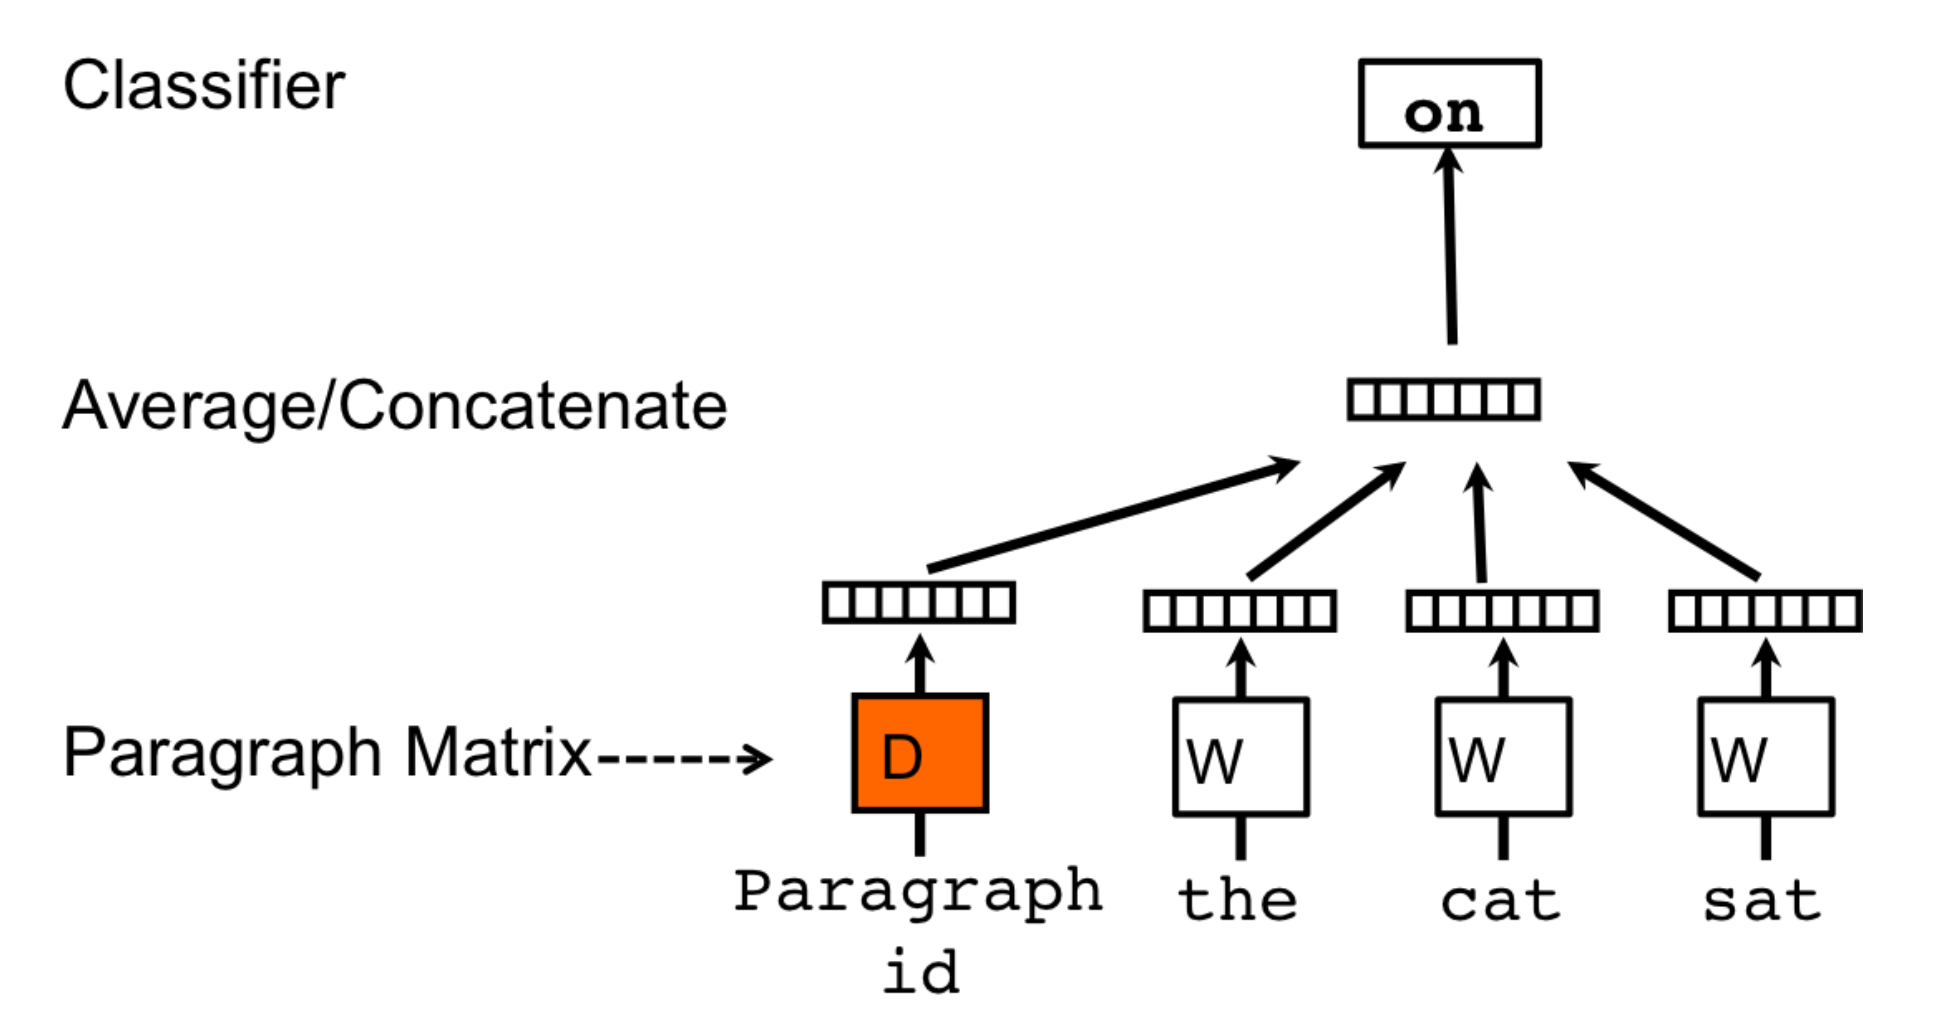
\includegraphics[width=0.3\textwidth]{figures/neural_models_distributed_memory.png}
				\caption{Distributed memory model. }
				\label{img:neural_models_distributed_memory}
			\end{figure}
		\end{itemize}
		\item Second method: \textit{Distributed bag of words}
		\begin{itemize}
			\item In this approach, we don't consider the context words but try to predict all possible words in the paragraph given the embedding vector
			\item This is done by sampling a random word at every SGD iteration from the small text windows, and train the classifier on predicting this word
			\item Thus, we optimize the embedding regarding representing the word distribution in the paragraph
			\item The distributed BOW is visualized in Figure~\ref{img:neural_model_distributed_BOW}
			\begin{figure}[ht]
				\centering
				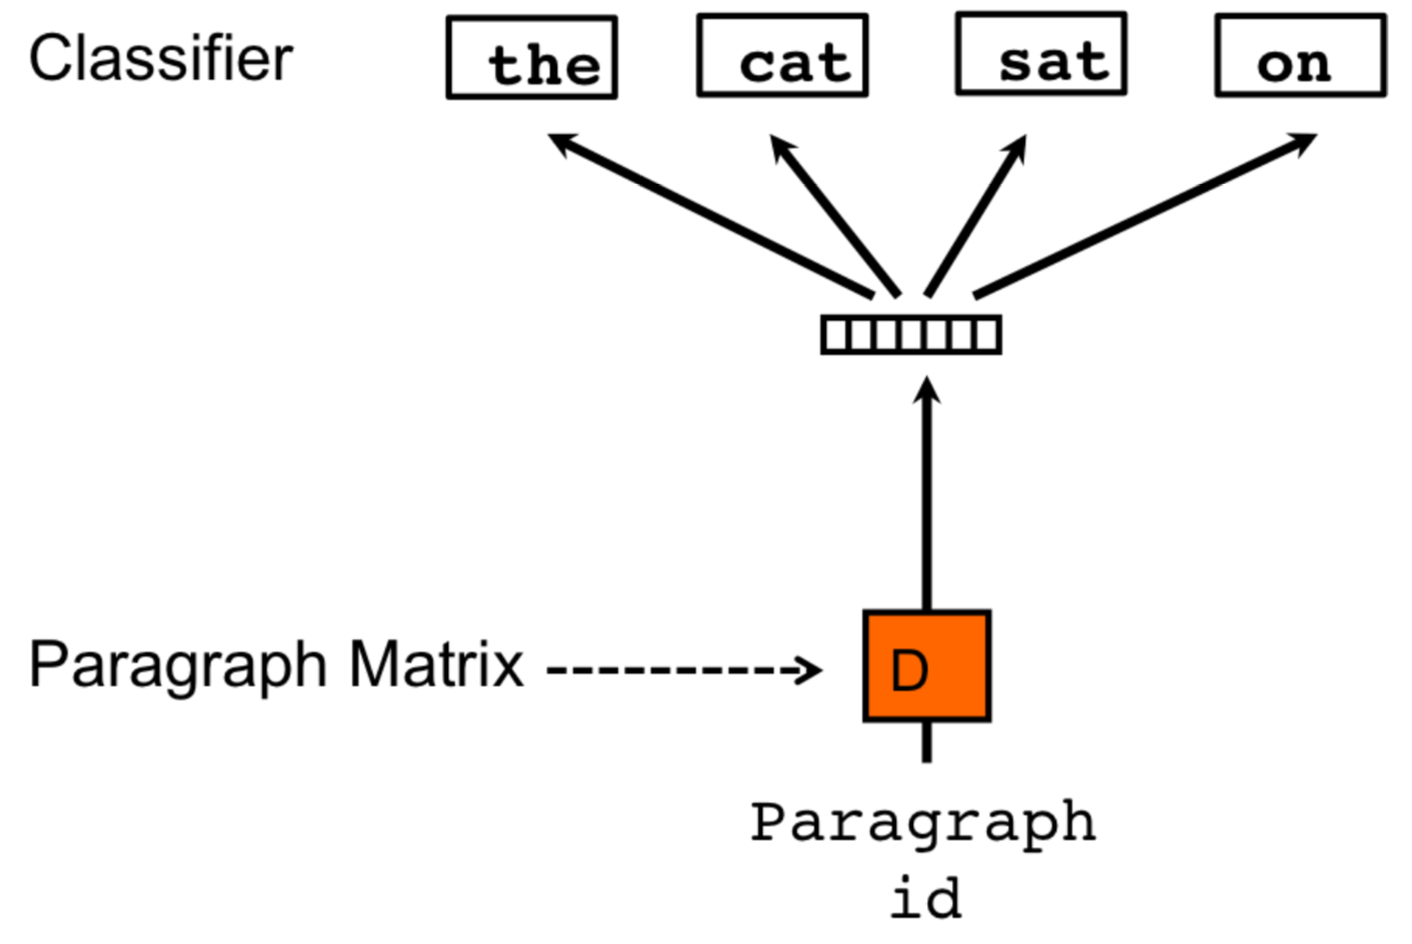
\includegraphics[width=0.3\textwidth]{figures/neural_model_distributed_BOW.png}
				\caption{Distributed BOW model. }
				\label{img:neural_model_distributed_BOW}
			\end{figure}
		\end{itemize}
	\end{itemize}
	\item \textbf{Lexicographical definition}
	\begin{itemize}
		\item We can also use the lexicographical definitions of words to train and/or test the word embeddings
		\item The word embeddings of the definition are combined by an (arithmetic) function $f_c$, and compared to the embedding of the word to be defined
		\item The objective is to minimize the distance to the defined word, but maximize the distance to other words to distinguish between words
		\item An example is shown in Figure~\ref{img:neural_model_lexicographical_definition}
		\begin{figure}[ht]
			\centering
			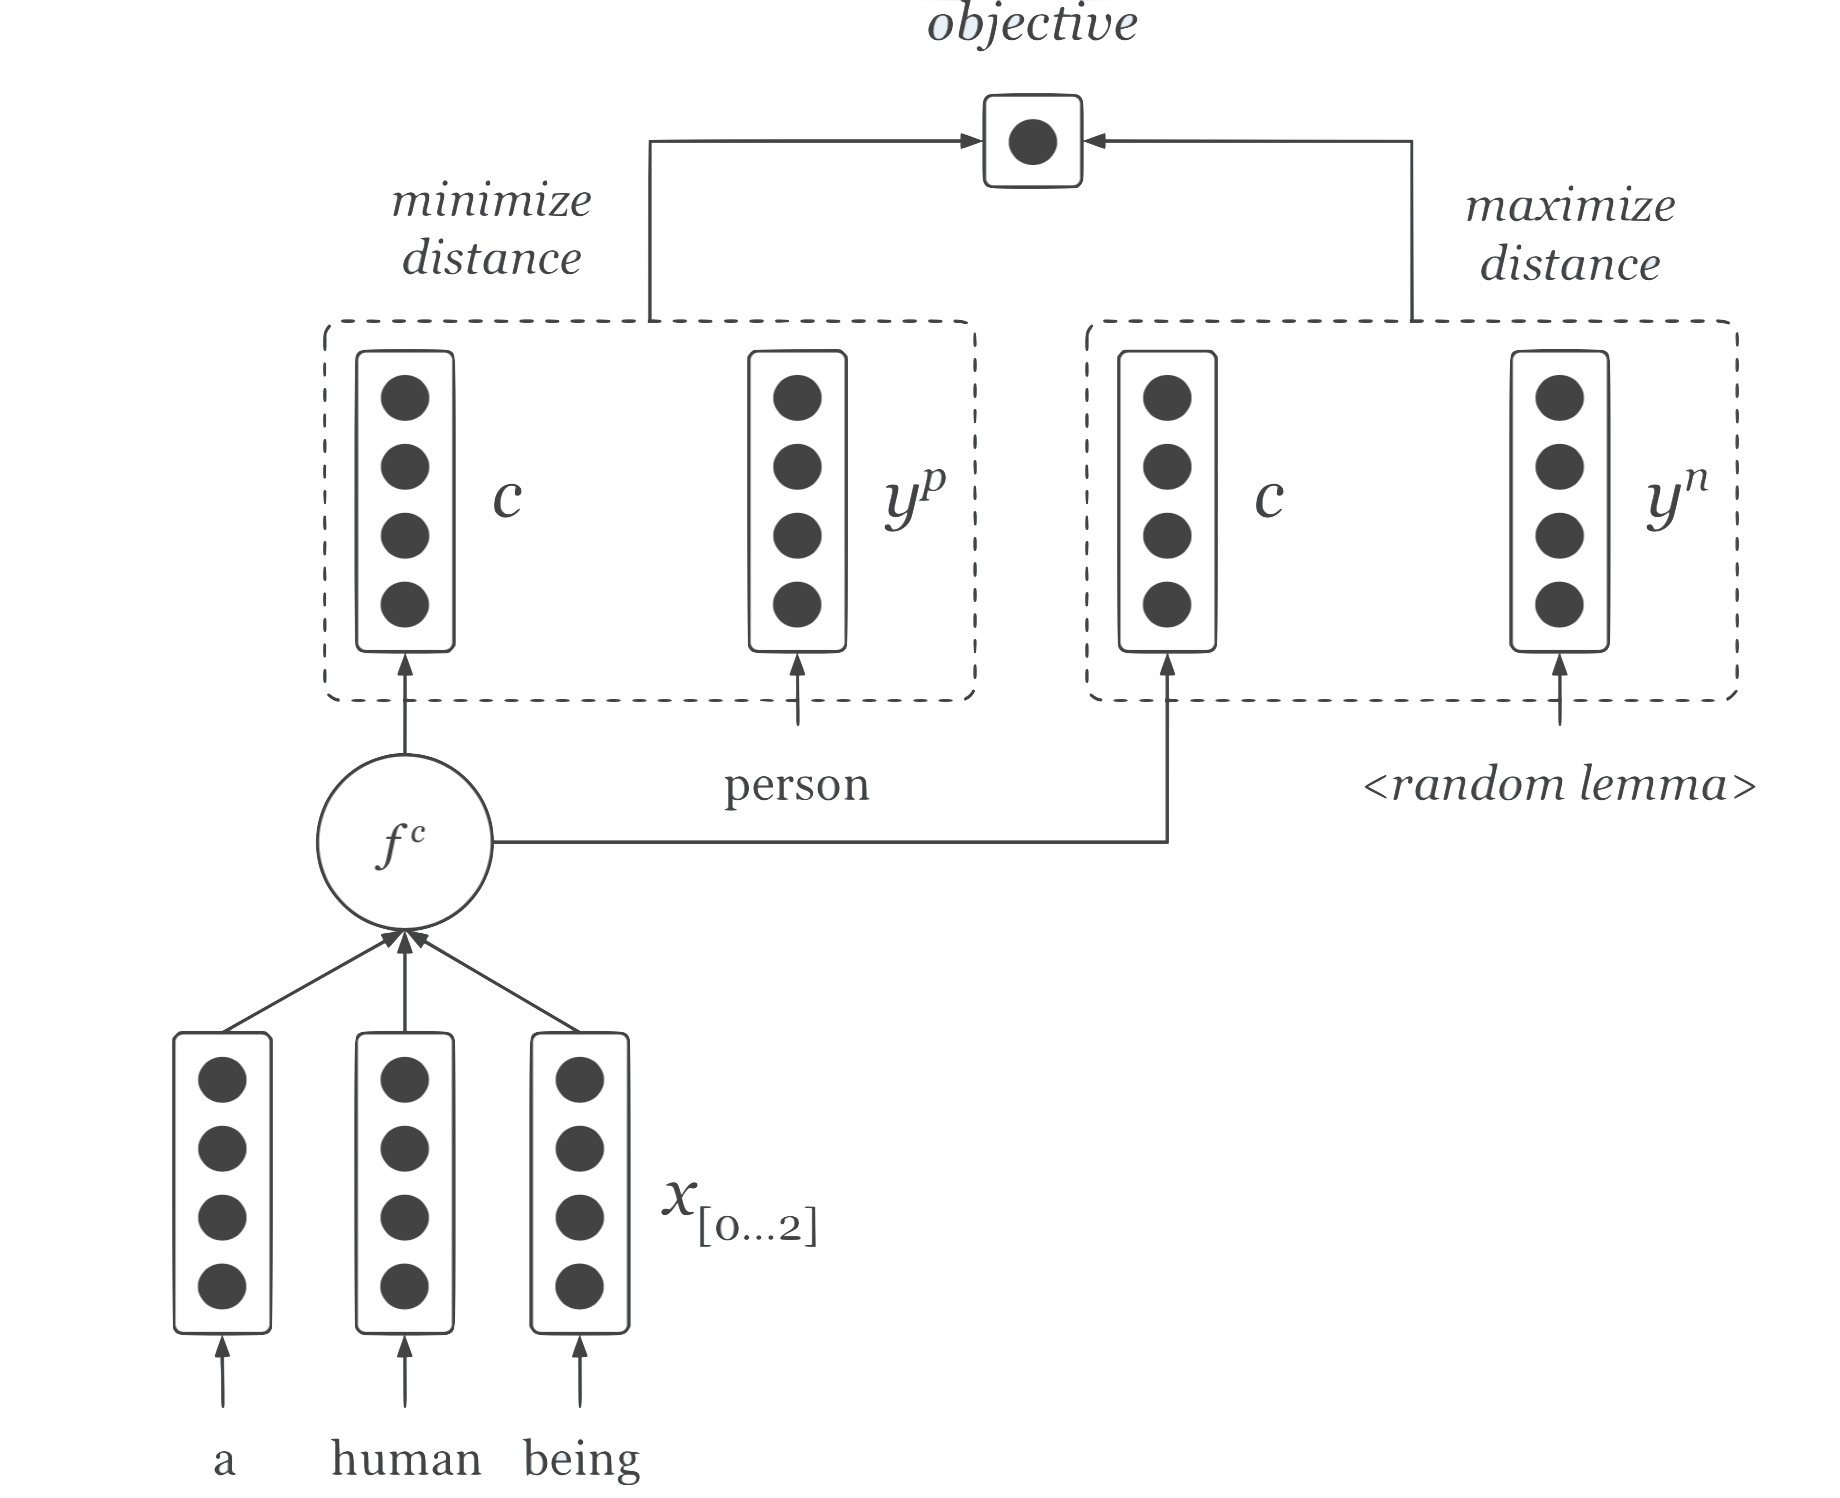
\includegraphics[width=0.3\textwidth]{figures/neural_model_lexicographical_definition.png}
			\caption{Lexicographical model for the example of "\textit{person}" defined as "\textit{a human being}". }
			\label{img:neural_model_lexicographical_definition}
		\end{figure}
	\end{itemize}
\end{itemize}
\subsubsection{Tune word vectors and learn rules of composition}
\begin{itemize}
	\item Deep, neural architectures which have different aspects to be designed
	\item \textbf{Architectures and representation}
	\begin{itemize}
		\item The simplest approach is to use neural networks to embed documents and queries to latent space, and then perform same similarity measures as before (like cosine similarity). This method is also referred to as \textit{Projection to latent space} (see Figure~\ref{img:neural_model_architecture_comparisons_projection_latent_space}). Possible network architectures are Convolutional NN, Recurrent NN or fixed Deep NNs if (max) input size is known
		\item The next step is to replace the similarity measure by another neural network. Thus, this NN takes the composed embeddings of the document and query as input, and return a single real value indicating the similarity score. This approach is called \textit{One Dimensional Matching} and visualized in Figure~\ref{img:neural_model_architecture_comparisons_one_dim_matching}. The common architecture for the highest 
		\item Another architecture is spanning up a two-dimensional input by the query and document. Therefore, we compute similarity scores for every word in the query to every word in the document which results in a two dimensional matrix. On this, we apply a convolutional NN to end up in a fixed-size embedding. A consecutive fully-connected NN maps this embedding into a similarity score. Figure~\ref{img:neural_model_architecture_comparisons_two_dim_matching} visualizes 
	\end{itemize}
	\begin{figure}[ht]
		\centering
		\begin{subfigure}[b]{0.3\textwidth}
			\centering
			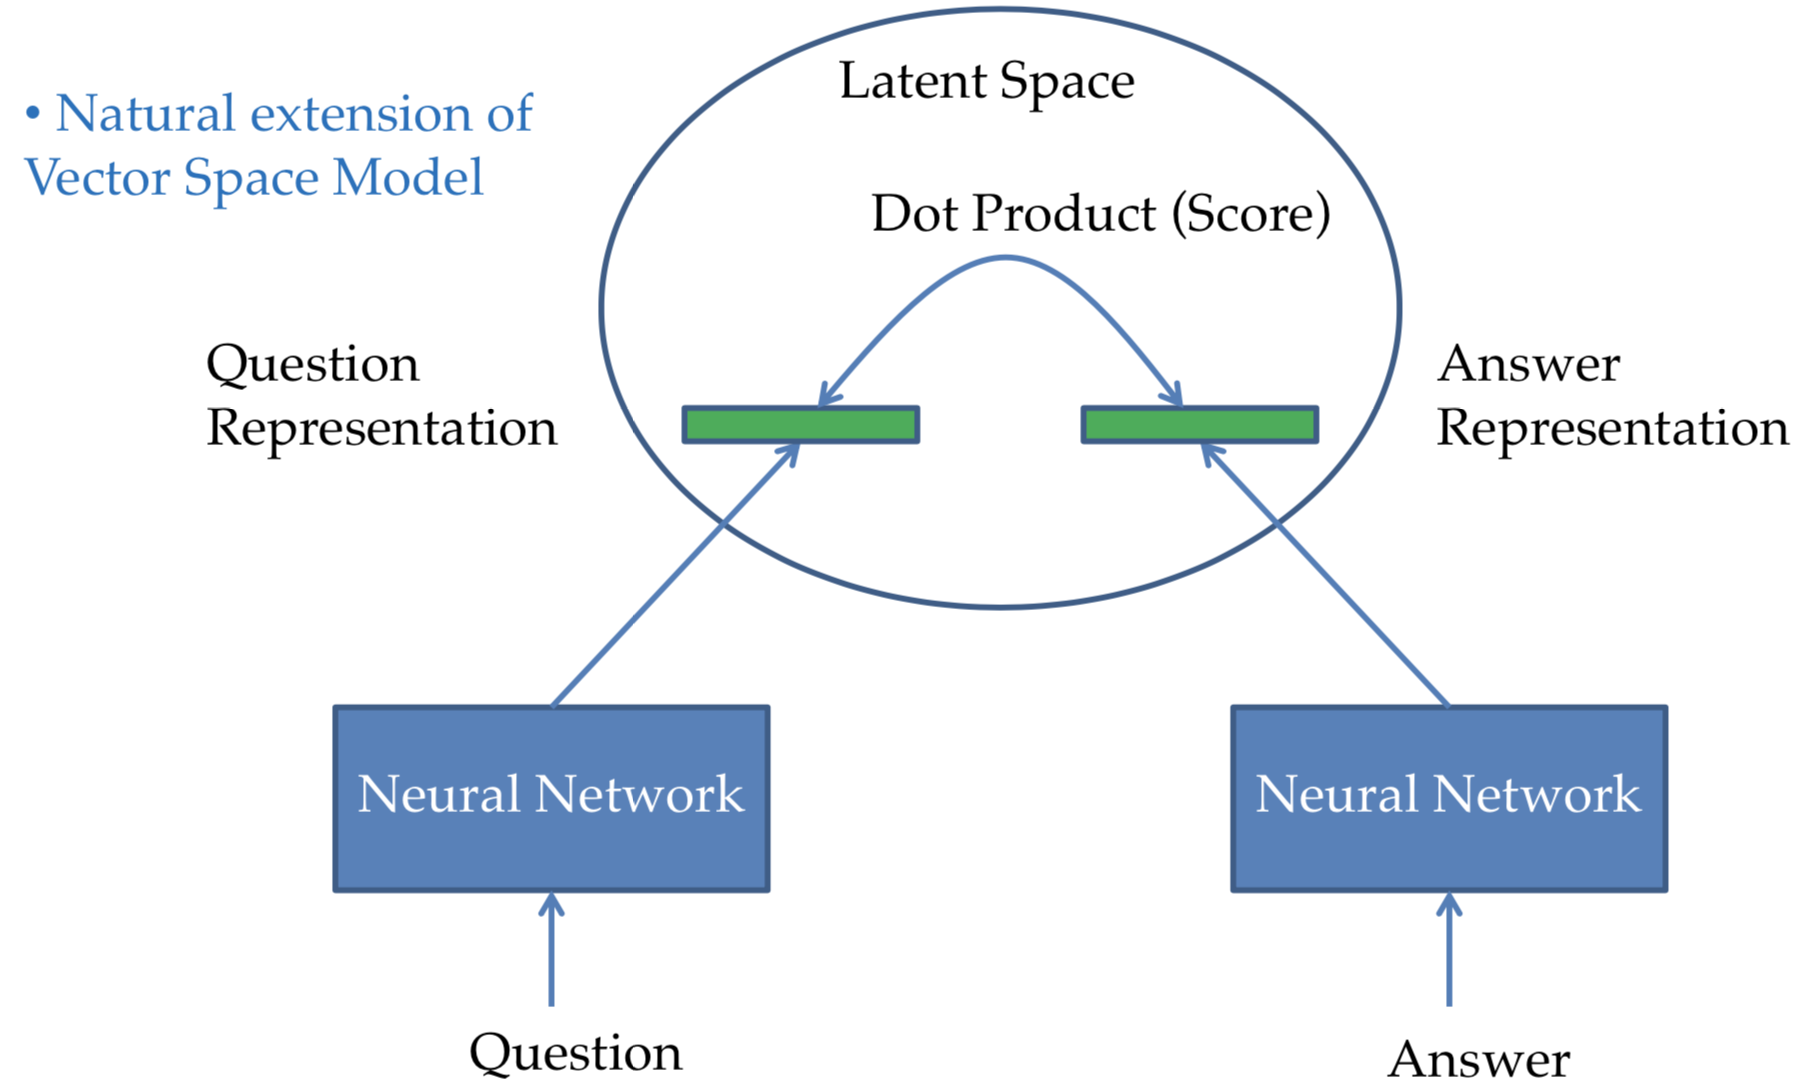
\includegraphics[width=\textwidth]{figures/neural_model_latent_space.png}
			\caption{Projection to Latent space}
			\label{img:neural_model_architecture_comparisons_projection_latent_space}
		\end{subfigure}
		\hspace{2mm}
		\begin{subfigure}[b]{0.3\textwidth}
			\centering
			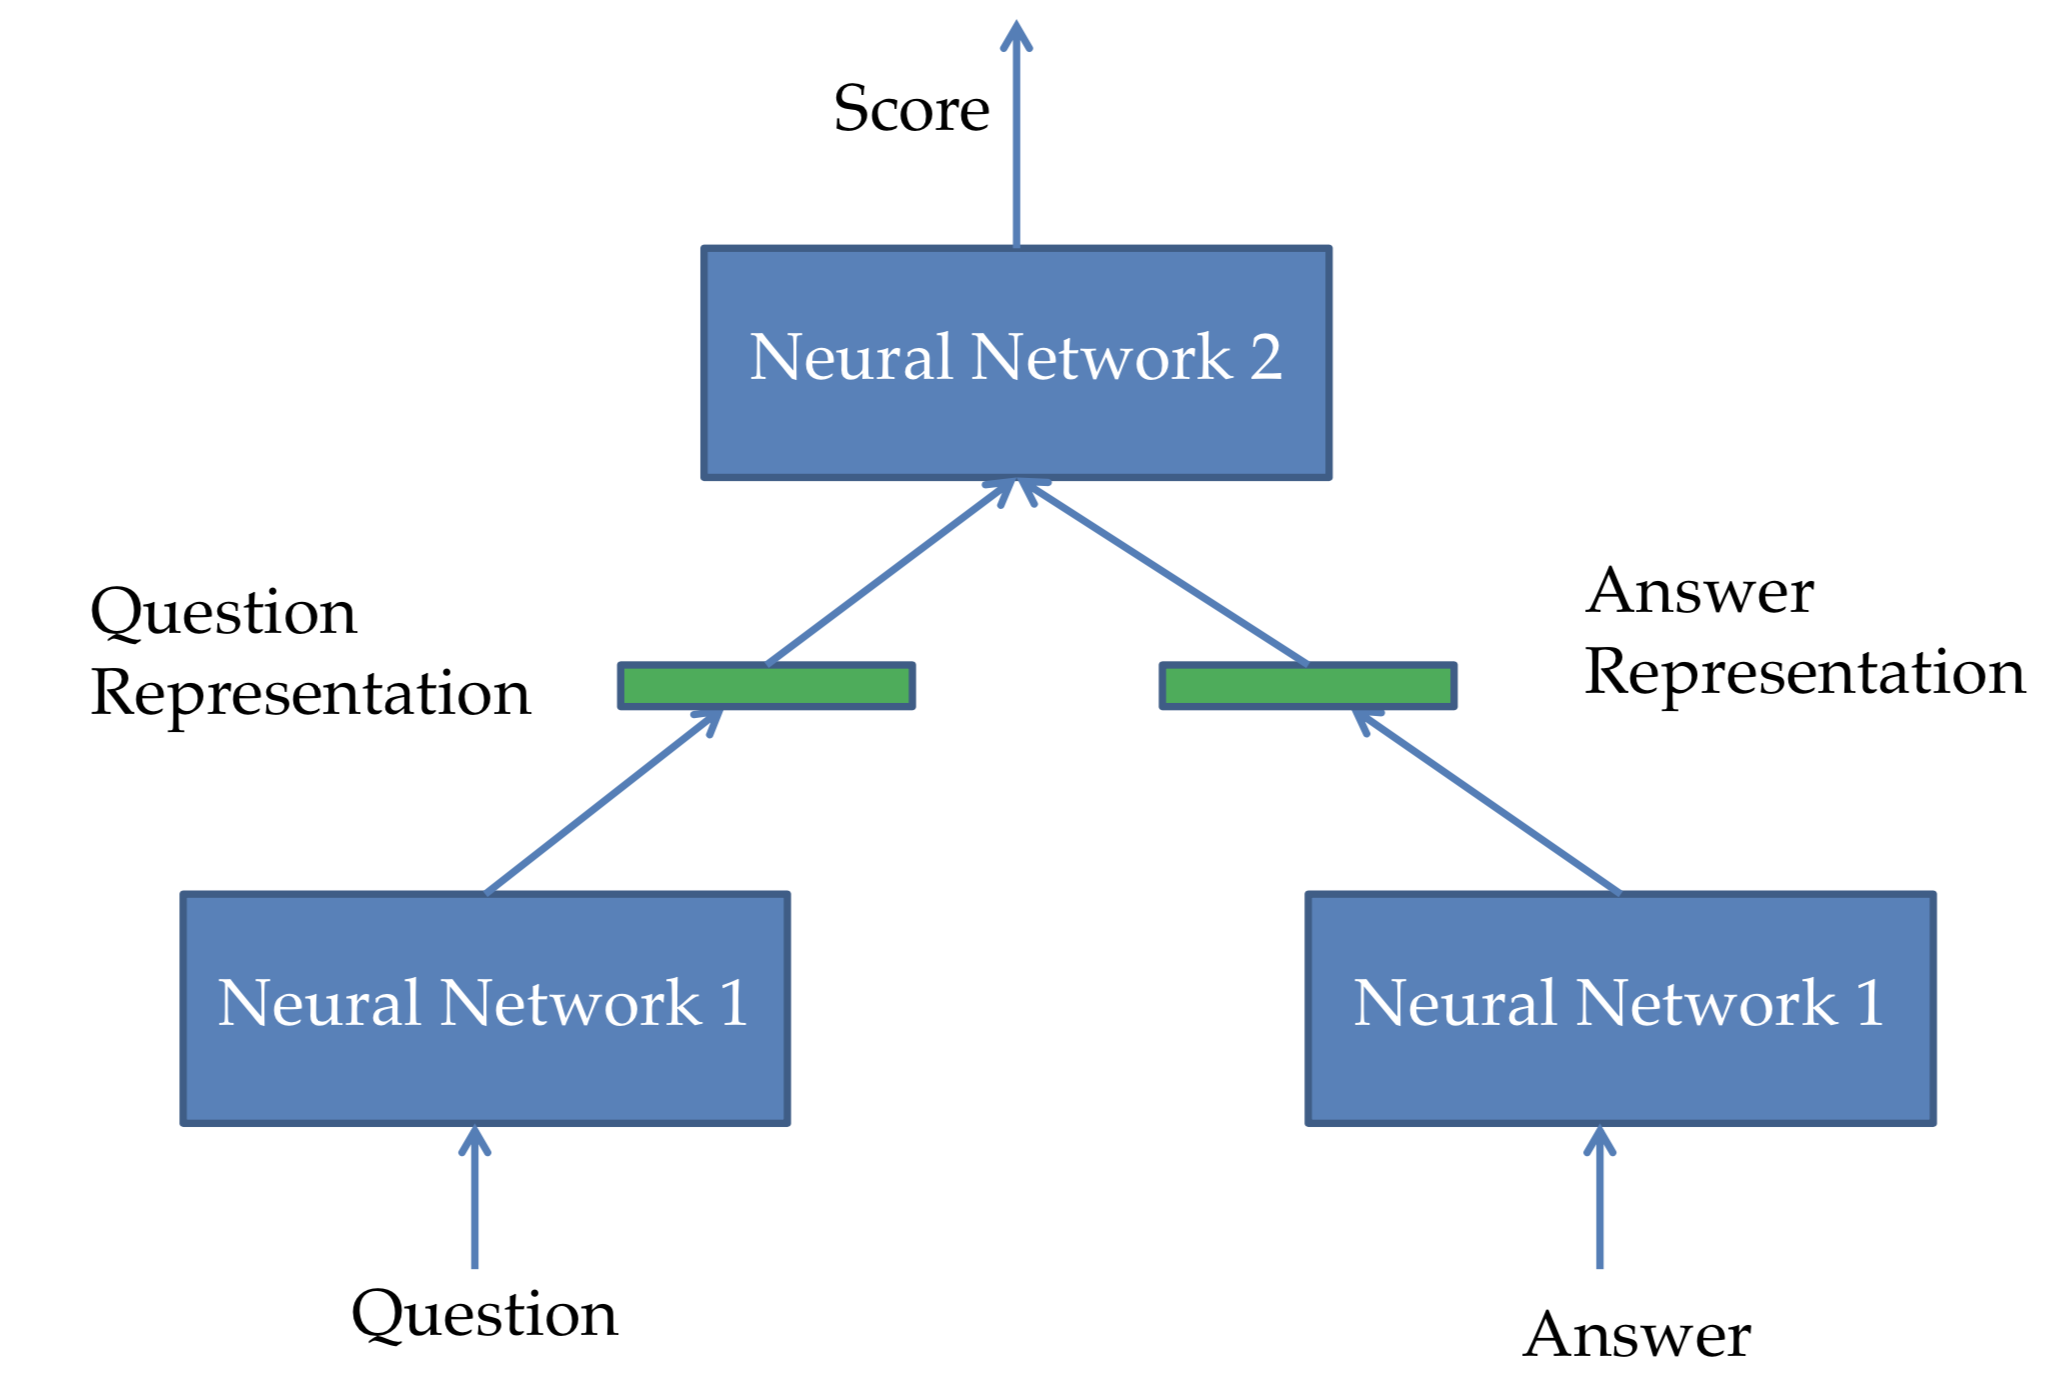
\includegraphics[width=\textwidth]{figures/neural_models_one_dimensional_matching.png}
			\caption{One dimensional matching}
			\label{img:neural_model_architecture_comparisons_one_dim_matching}
		\end{subfigure}
		\hspace{2mm}
		\begin{subfigure}[b]{0.3\textwidth}
			\centering
			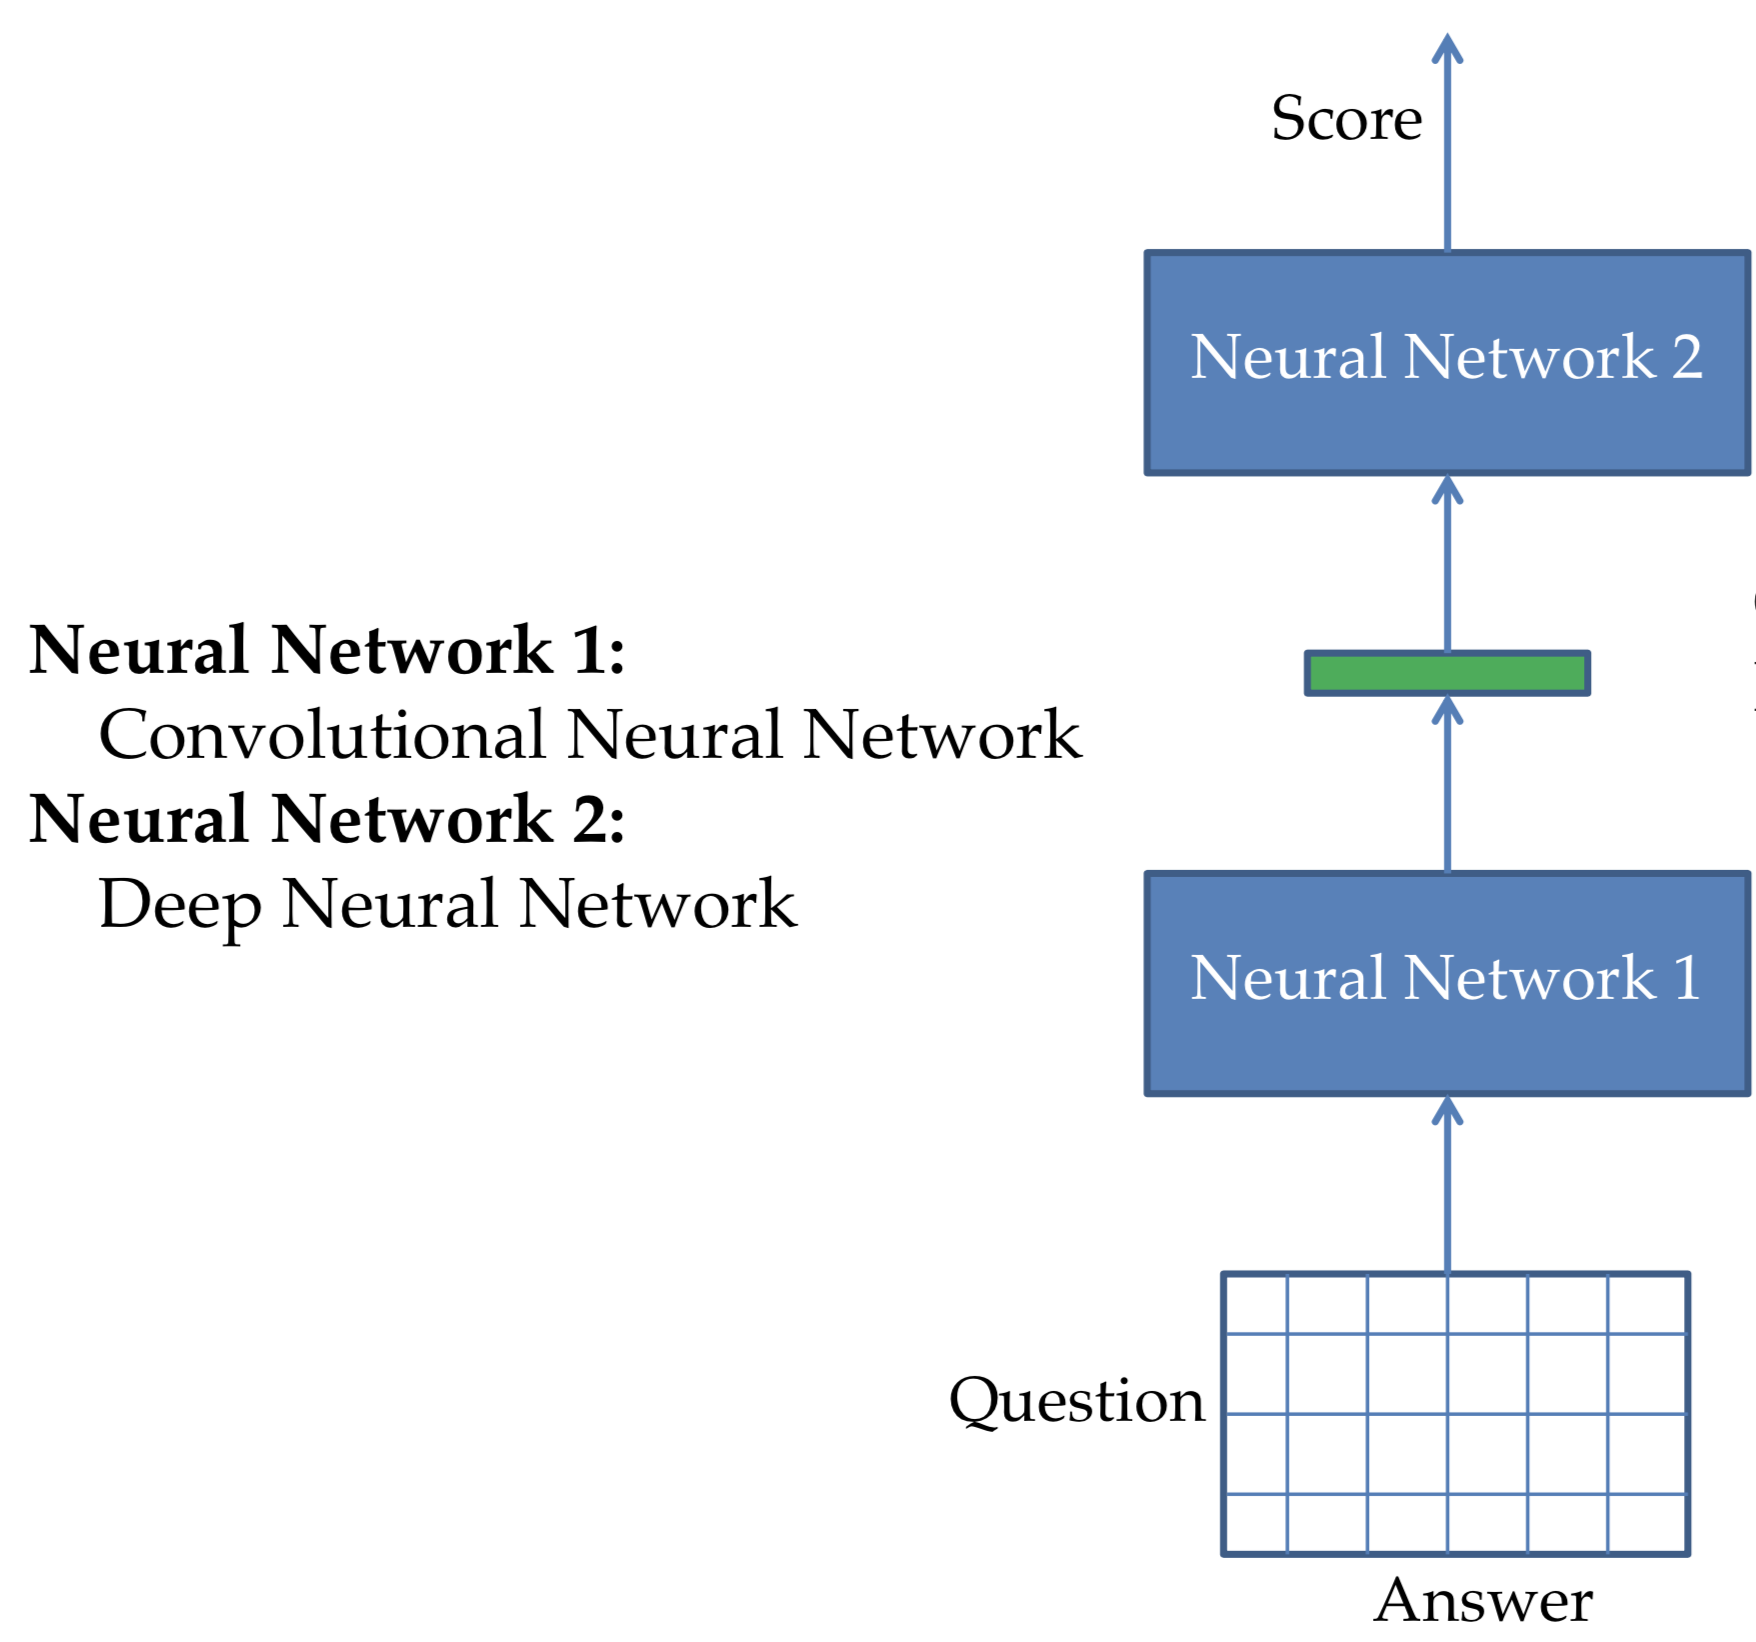
\includegraphics[width=0.8\textwidth]{figures/neural_models_two_dim_matching.png}
			\caption{Two dimensional matching}
			\label{img:neural_model_architecture_comparisons_two_dim_matching}
		\end{subfigure}
		\label{img:neural_model_architecture_comparisons}
		\caption{Comparison of different neural architectures for compositionality}
	\end{figure}
	\item \textbf{Training}: depending on the available data, we can perform different levels of supervision
	\begin{itemize}
		\item \textit{No supervision/labels}: If no labels are provided at all, we could autoencoders to reduce query and document to a latent space and check similarity metrics. Otherwise, we can make use of pretrained neural language models with techniques like ELMo and BERT
		\item \textit{Distant supervision}: We create pseudo-labels by sampling short word sequences from a document and considering this as query. The document from which we sampled is labeled as relevant/high similarity, while all other documents (from which we sample one randomly for training) are considered as being not relevant
		\item \textit{Weak supervision}: As alternative, we can use unsupervised ranking functions like BM25 to generate labels and use this scores for training (teacher-student architecture). In experiments, the neural network was even able to outperform BM25.
		\item \textit{Full supervision}: Labels are created by either annotators or using the click log as implicit feedback from the users. We can train the models in a standard supervised fashion. 
	\end{itemize}
\end{itemize}
\section{Learning to Rank}
\begin{itemize}
	\item Main issue in information retrieval is to determine whether document $d$ is relevant for query $q$
	\item Common relevance signals include TF-IDF, BM25, document popularity etc.
	\item But: what signals to use/how to combine these signals? There is not a single relevance signal "to rule them all" $\implies$ combine all signals in a model
	\item Simplest combination method: linear model $f(\bm{d},\bm{\theta}) = \sum\limits_{i=1}^{|d|} \theta_i d_i$ where $\bm{d}$ represents the different signals for document-query pair
	\item Task: find the optimal parameter set $\bm{\theta}$, commonly by Machine Learning techniques (linear regression)
\end{itemize}
\subsection{Offline Learning To Rank}
\begin{itemize}
	\item Given an annotated dataset of relation document and relevance/ranking
	\item There are three different approaches
	\begin{enumerate}
		\item \textbf{Pointwise}: optimize models $f(\bm{d},\bm{\theta})$ to predict relevancy of a document. This can be recasted in a regression problem with loss:
		$$\mathcal{L}=\sum_{\bm{d}} \left(f(\bm{d},\bm{\theta}) - \text{relevancy}(d,q)\right)^2$$
		However, this approach does not consider the application of ranking where only the final order is important, but not the single scores.
		\item \textbf{Pairwise}: optimize regarding the total order of the documents and not specific relevance scores. The loss can be expressed by:
		$$\mathcal{L}=\sum_{d\succ d'}\left[f(\bm{d'},\bm{\theta}) - f(\bm{d},\bm{\theta})\right]$$ 
		where $d\succ d'$ means that $d'$ is the successor of $d$ in the labeled ranking. Nevertheless, this method does not take into account that only a subpart (top 10) of the collection is actually presented to the user.
		\item \textbf{Listwise}: optimize regarding ranking metrics like $DCG$. Thus, the loss could be:
		$$\mathcal{L} = -nDCG(f(\cdot,\bm{\theta}))$$
		The problem is that most ranking metrics are not differentiable. There are heuristic approaches to still optimize with respect to such metrics. 
	\end{enumerate}
	\item Problems with offline Learning to Rank: similar to offline evaluation in Section~\ref{sec:offline_eval_problems}
	\begin{itemize}
		\item All described methods require an annotated dataset which contains either relevance labels for each document-query pair or a ranking over the whole collection.
		\item Creating such is time consuming and expensive
		\item Impossible to personalize for a user (everyone prefers a little bit different documents). Also, annotators and users might disagree in some points $\implies$ dataset does not fully reflect user behavior
		\item Can change over time
	\end{itemize}
\end{itemize}
\subsection{Online Learning to Rank}
\begin{itemize}
	\item Learn from implicit user feedback
	\begin{itemize}
		\item Might be noisy
		\item Consider position bias (higher rank is more frequently clicked) and selection bias (only a limited set of documents is presented to the user)
	\end{itemize}
	\item Online Learning to Rank methods can learn from user interactions, \textbf{and} control the results which are displayed/presented to the user
	\item Thus, these methods can be more efficients as they control over what data is actually gathered
	\item A general online learning to rank technique is visualized in Figure~\ref{img:learning_to_rank_online_overview}
	\begin{figure}[ht]
		\centering
		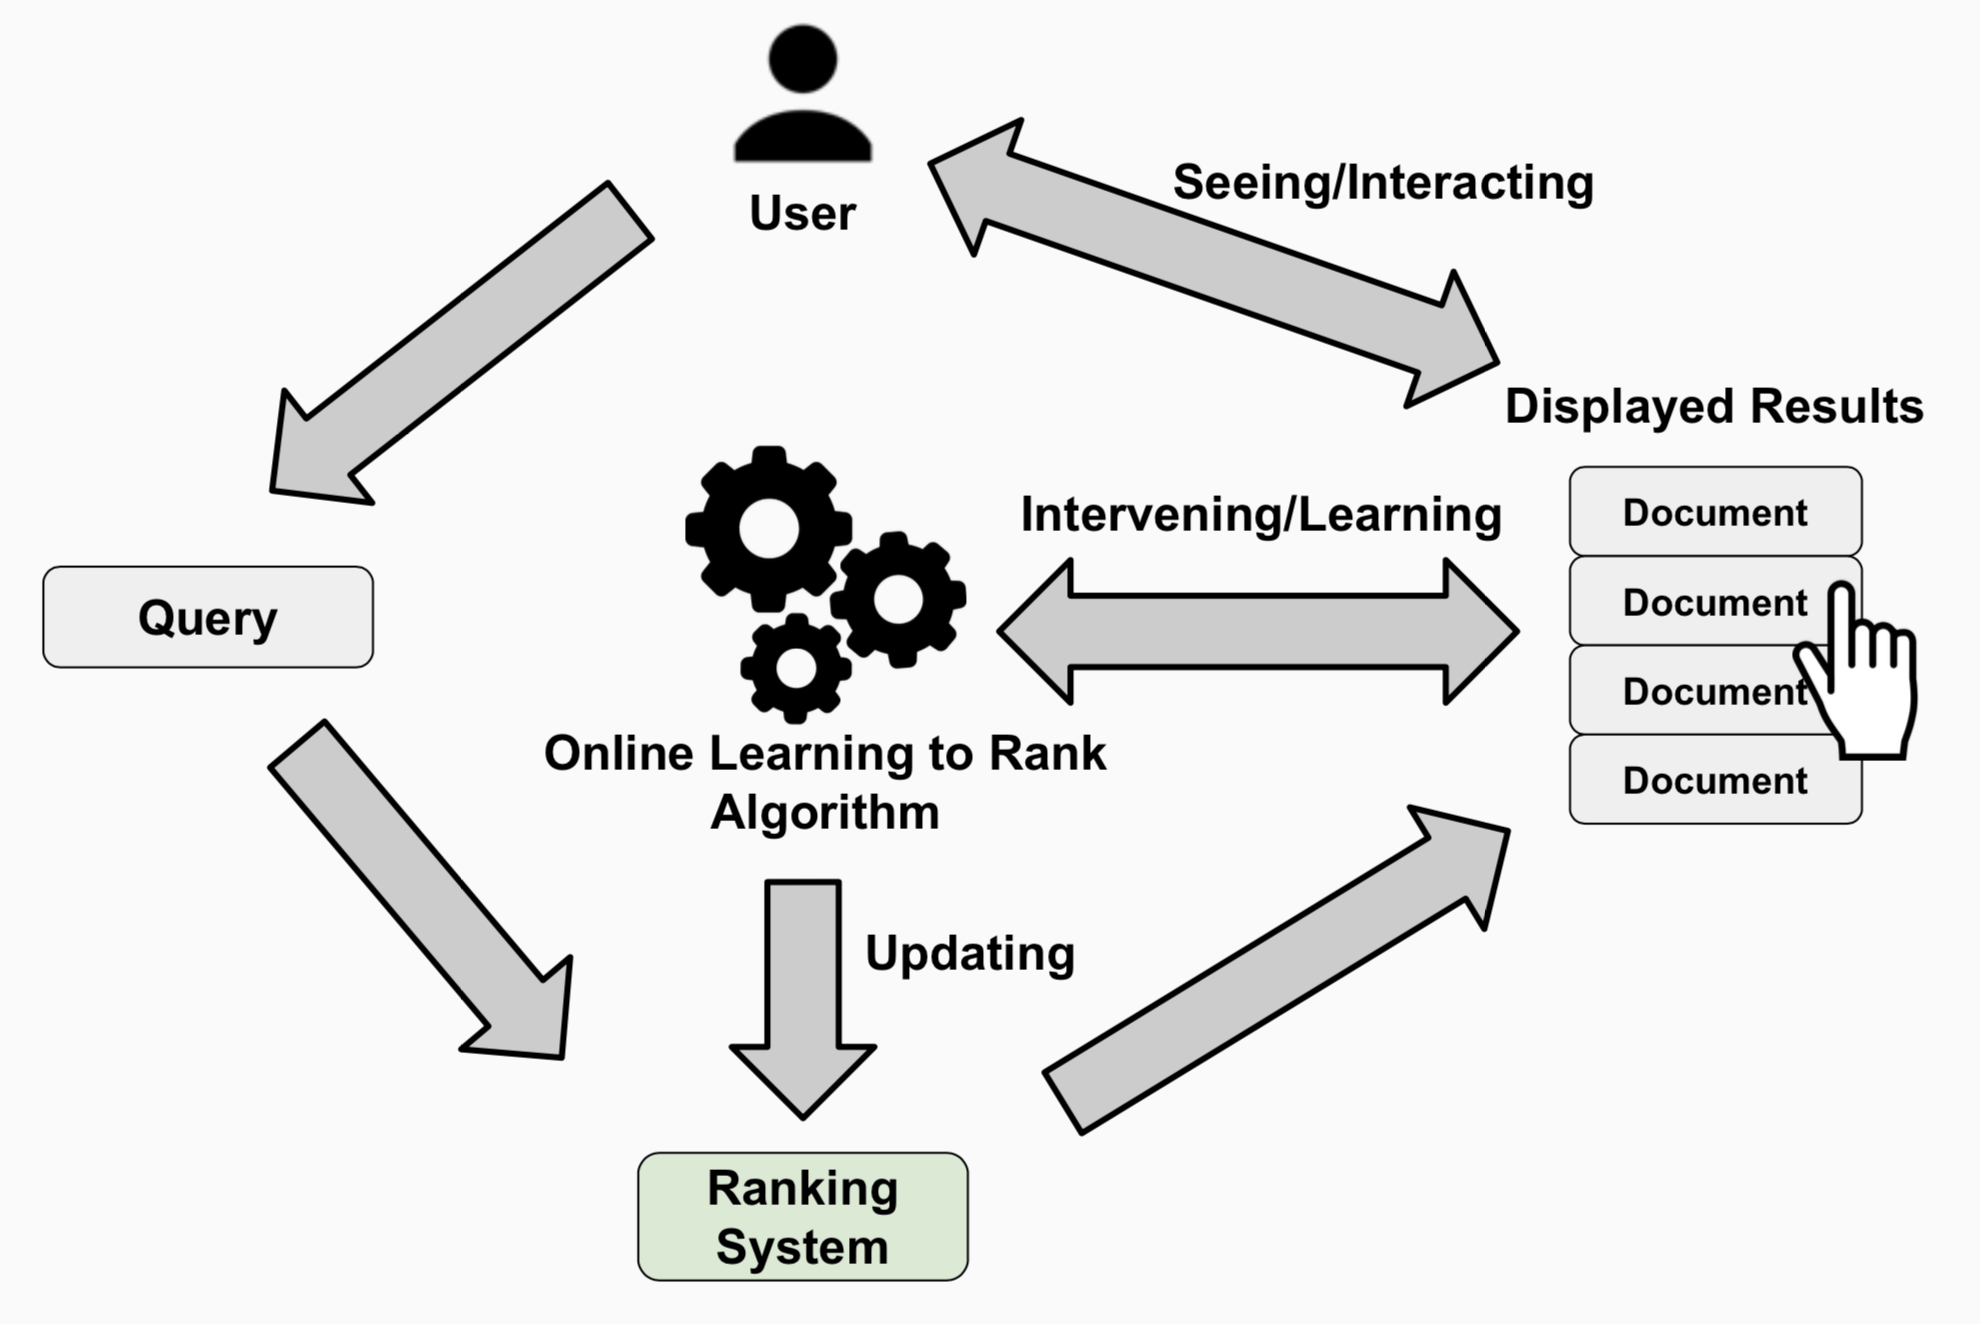
\includegraphics[width=0.4\textwidth]{figures/learning_to_rank_online_overview.png}
		\caption{Overview of the general concept of online learning to rank}
		\label{img:learning_to_rank_online_overview}
	\end{figure}
	\begin{itemize}
		\item The user enters a query, for which the ranking algorithm generates a list of documents
		\item The Online Learning to Rank system interacts with the results by adding and/or removing documents from the ranking. This can also include interleaving with another, slightly changed ranking algorithm
		\item User interacts with the displayed result and gives implicit feedback.
		\item The Online Learning to Rank algorithm updates the ranking parameters according to the analyzed feedback
	\end{itemize}
	\item \textbf{Advantages}: learns directly from the user, is more responsive by immediately adapting its parameters
	\item \textbf{Risks}:
	\begin{itemize}
		\item Unreliable methods will affect/worsen user experiences immediately.
		\item (Noisy) clicks can easily bias or even manipulate search engines
		\item \textbf{Self-confirming loop}
		\begin{itemize}
			\item If an irrelevant document was clicked by random, the system still perceives that this document is relevant and will change its parameters accordingly
			\item Thus, the random document will be placed higher in future ranks. However, also similar documents to the irrelevant one will have an increased relevance score and will probably occur at a high position
			\item Most likely, the next clicked document will be one of the highest ones which were irrelevant $\implies$ entering a self-confirming loop
			\item Due to bias and noise, an irrelevant document was clicked and inferred to be relevant
			\item Due to noise, this inference is most likely to appear again
			\item The algorithms confidence in this incorrect inference continues to increase
		\end{itemize}
	\end{itemize}
	\item To prevent a self-confirming loop, we have to balance exploration and exploitation
	\begin{itemize}
		\item \textit{Exploration}: collect feedback for learning from the most documents as possible
		\item \textit{Exploitation}: utilize what has been already learned 
		\item If systems only exploits, it misses out to obtain feedback for other documents that might be even better (danger to enter/staying in self-confirming loop)
		\item To high exploration rate leads to a lot of irrelevant documents in ranking that worsen the user experience 
	\end{itemize}
\end{itemize}
\subsubsection{Designing an Online Learning to Rank algorithm}
\begin{itemize}
	\item To design a OLTR algorithm, we have to make design choices in four aspects (see Figure~\ref{img:learning_to_rank_online_design})
\end{itemize}
\begin{figure}[ht]
	\centering
	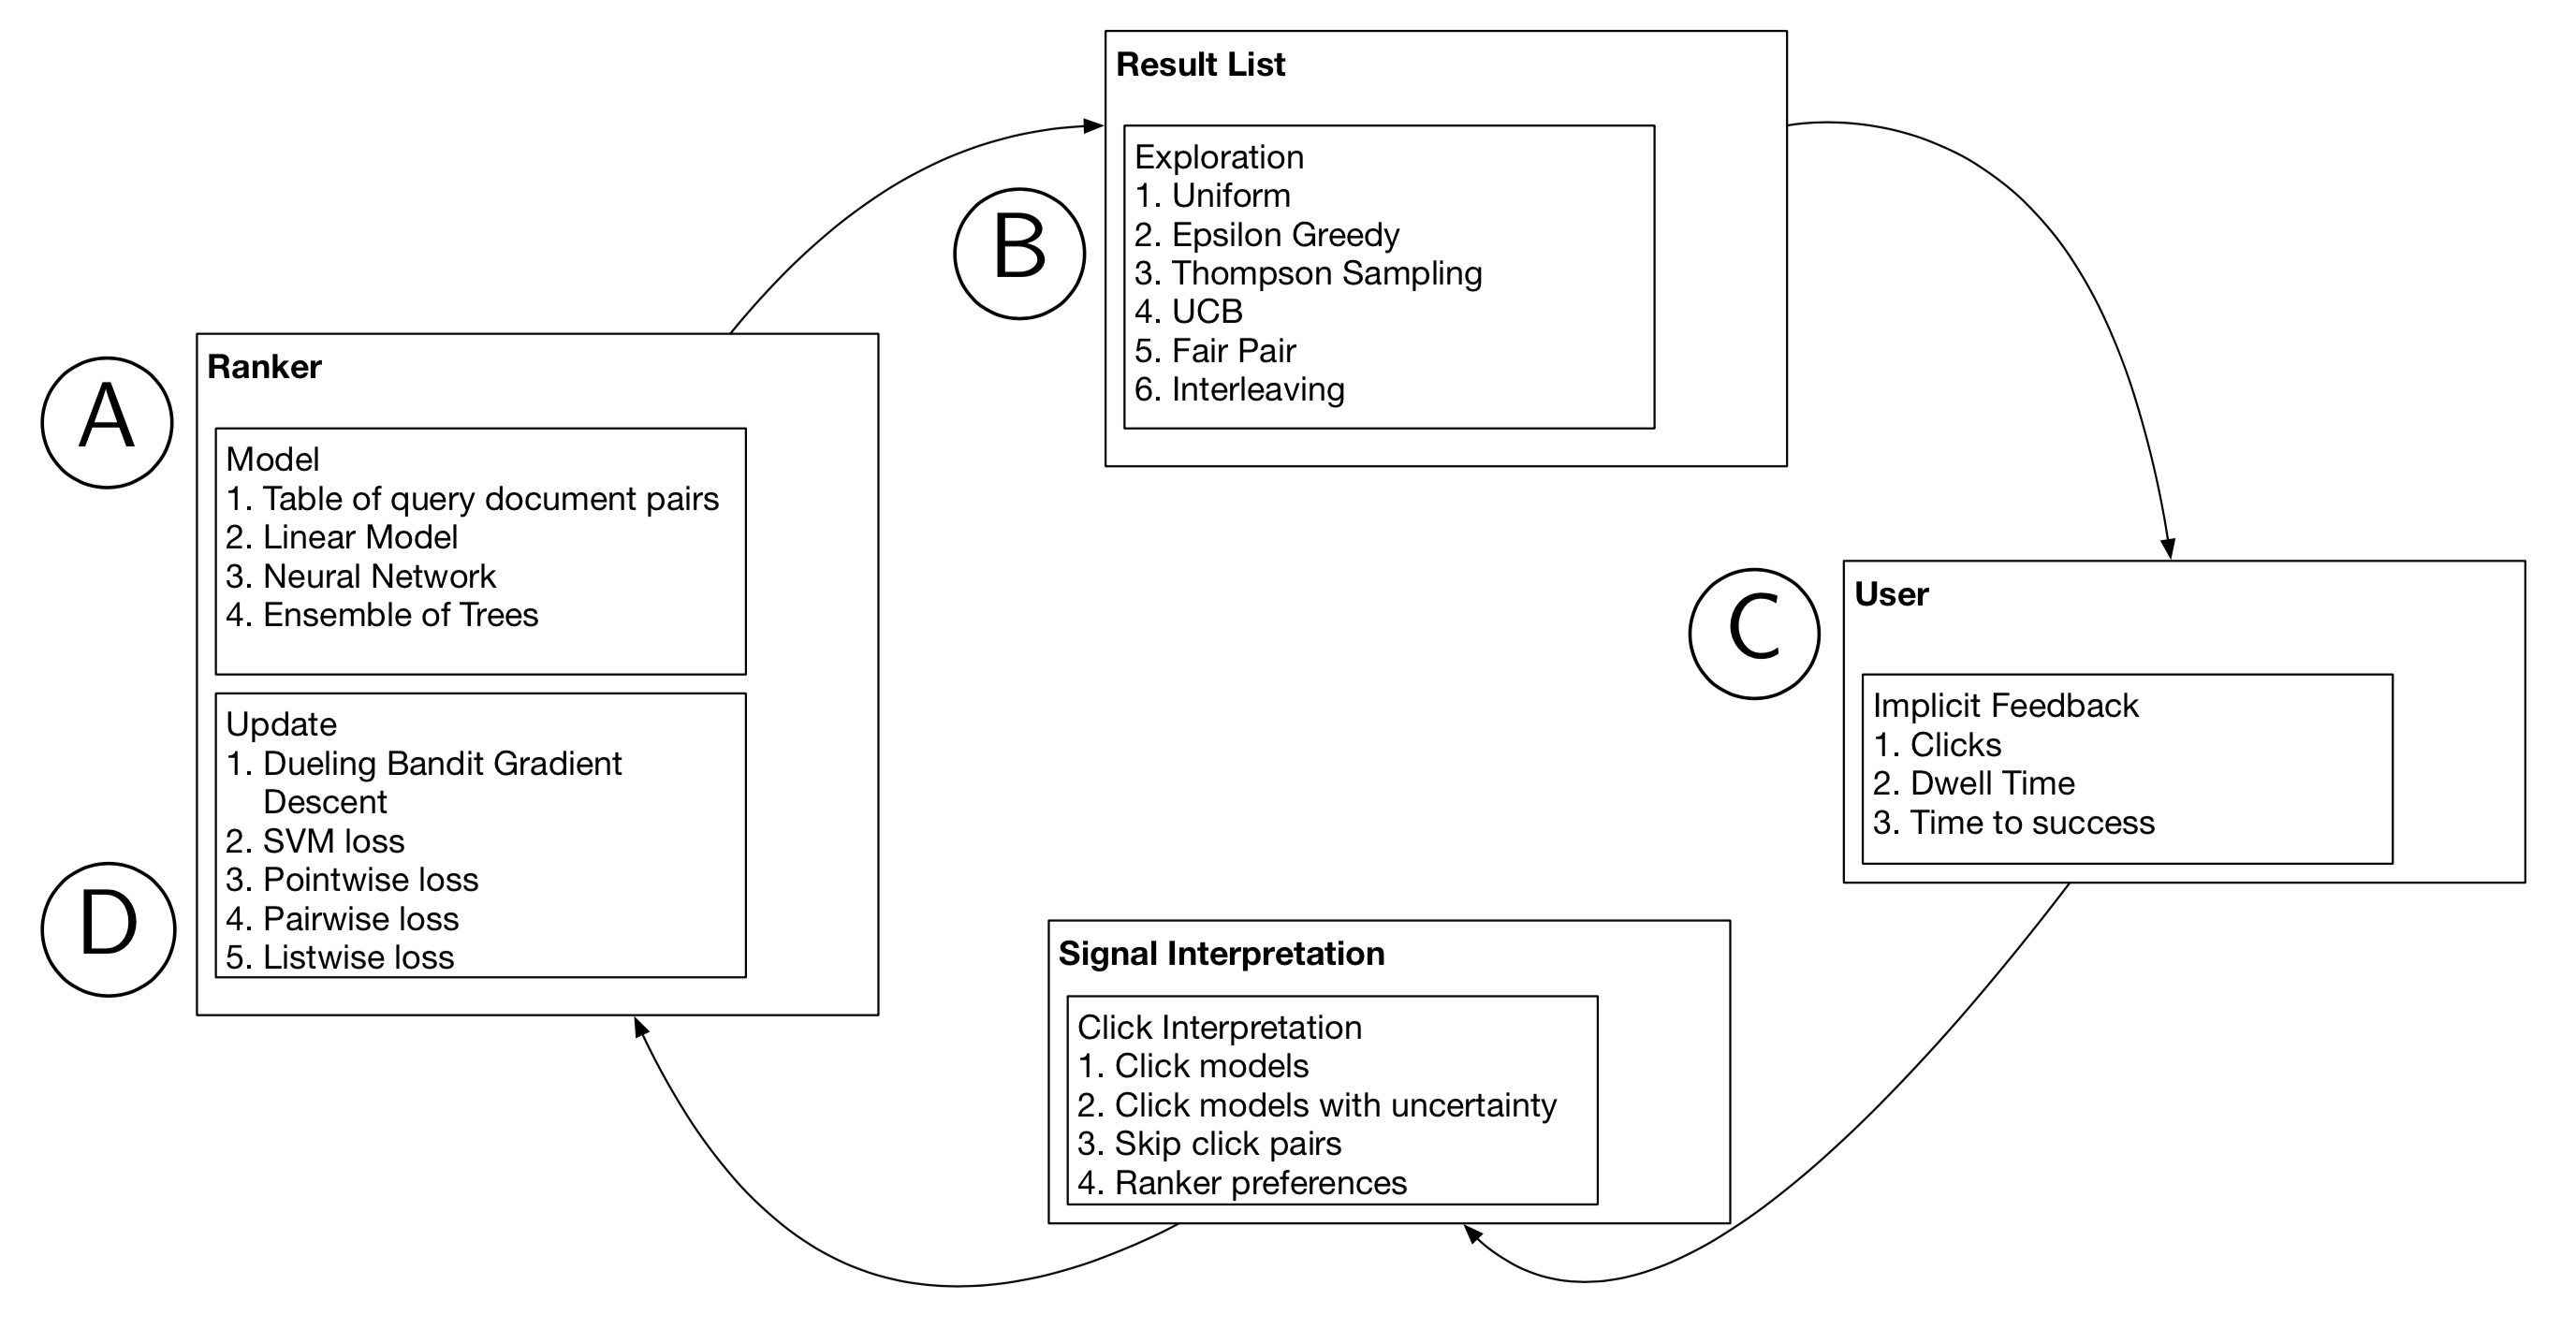
\includegraphics[width=0.4\textwidth]{figures/learning_to_rank_online_design.png}
	\caption{General design components of an OLTR algorithm}
	\label{img:learning_to_rank_online_design}
\end{figure}
\begin{enumerate}[label=(\Alph*)]
	\item \textbf{Ranker}: the ranker maps documents to relevance scores. This module operates on feature level/document id's and can be for example a linear ranker/neural model/...
	\item \textbf{Exploration strategy}: define interactions with results of the ranker. No exploration would mean that the document ranking is simply passed and stays unchanged. A common strategy is \textit{epsilon-greedy} where we inject random documents in random positions with ratio $\epsilon$. Other algorithms include upper confidence bound etc.
	\item \textbf{Signal recording and interpretation}: algorithm can consider multiple signals (raw observation like clicks and dwell time, more complex metrics like time to success). Should remove bias/noise. When result list was constructed by using interleaving, the feedback would also consider which ranker has won based on user interactions.
	\item \textbf{Update mechanism}: update ranking algorithm given the user feedback. If ranker operates on document id's, we can update the document's specific relevance estimate for the query. If the ranker relies on features, we optimize a loss function like the ones shown in offline LTR.
\end{enumerate}
\subsubsection{Dueling Bandit Gradient Descent}
\begin{itemize}
	\item One of the first OLTR algorithms was the \textit{Dueling Bandit Gradient Descent}
	\item The intuition is that we compare two rankers by online evaluation, and optimize our system towards the better performing one.
	\item The method is structured in following steps (visualized in Figure~\ref{img:learning_to_rank_online_DBGD})
	\begin{enumerate}
		\item From current feature state $\theta_b$ of the ranker (shown in green), sample a new ranker/feature point $\theta_c = \theta_b + u$ laying on the unit sphere $||u||=1$ around the current one (shown in red)
		\item Get the rankings of $\theta_b$ and $\theta_c$
		\item Compare $\theta_b$ and $\theta_c$ using interleaving
		\item If $\theta_c$ wins comparison: update the current model by $\theta_b \leftarrow \theta_b + \eta (\theta_c - \theta_b)$
	\end{enumerate}
	\begin{figure}[ht]
		\centering
		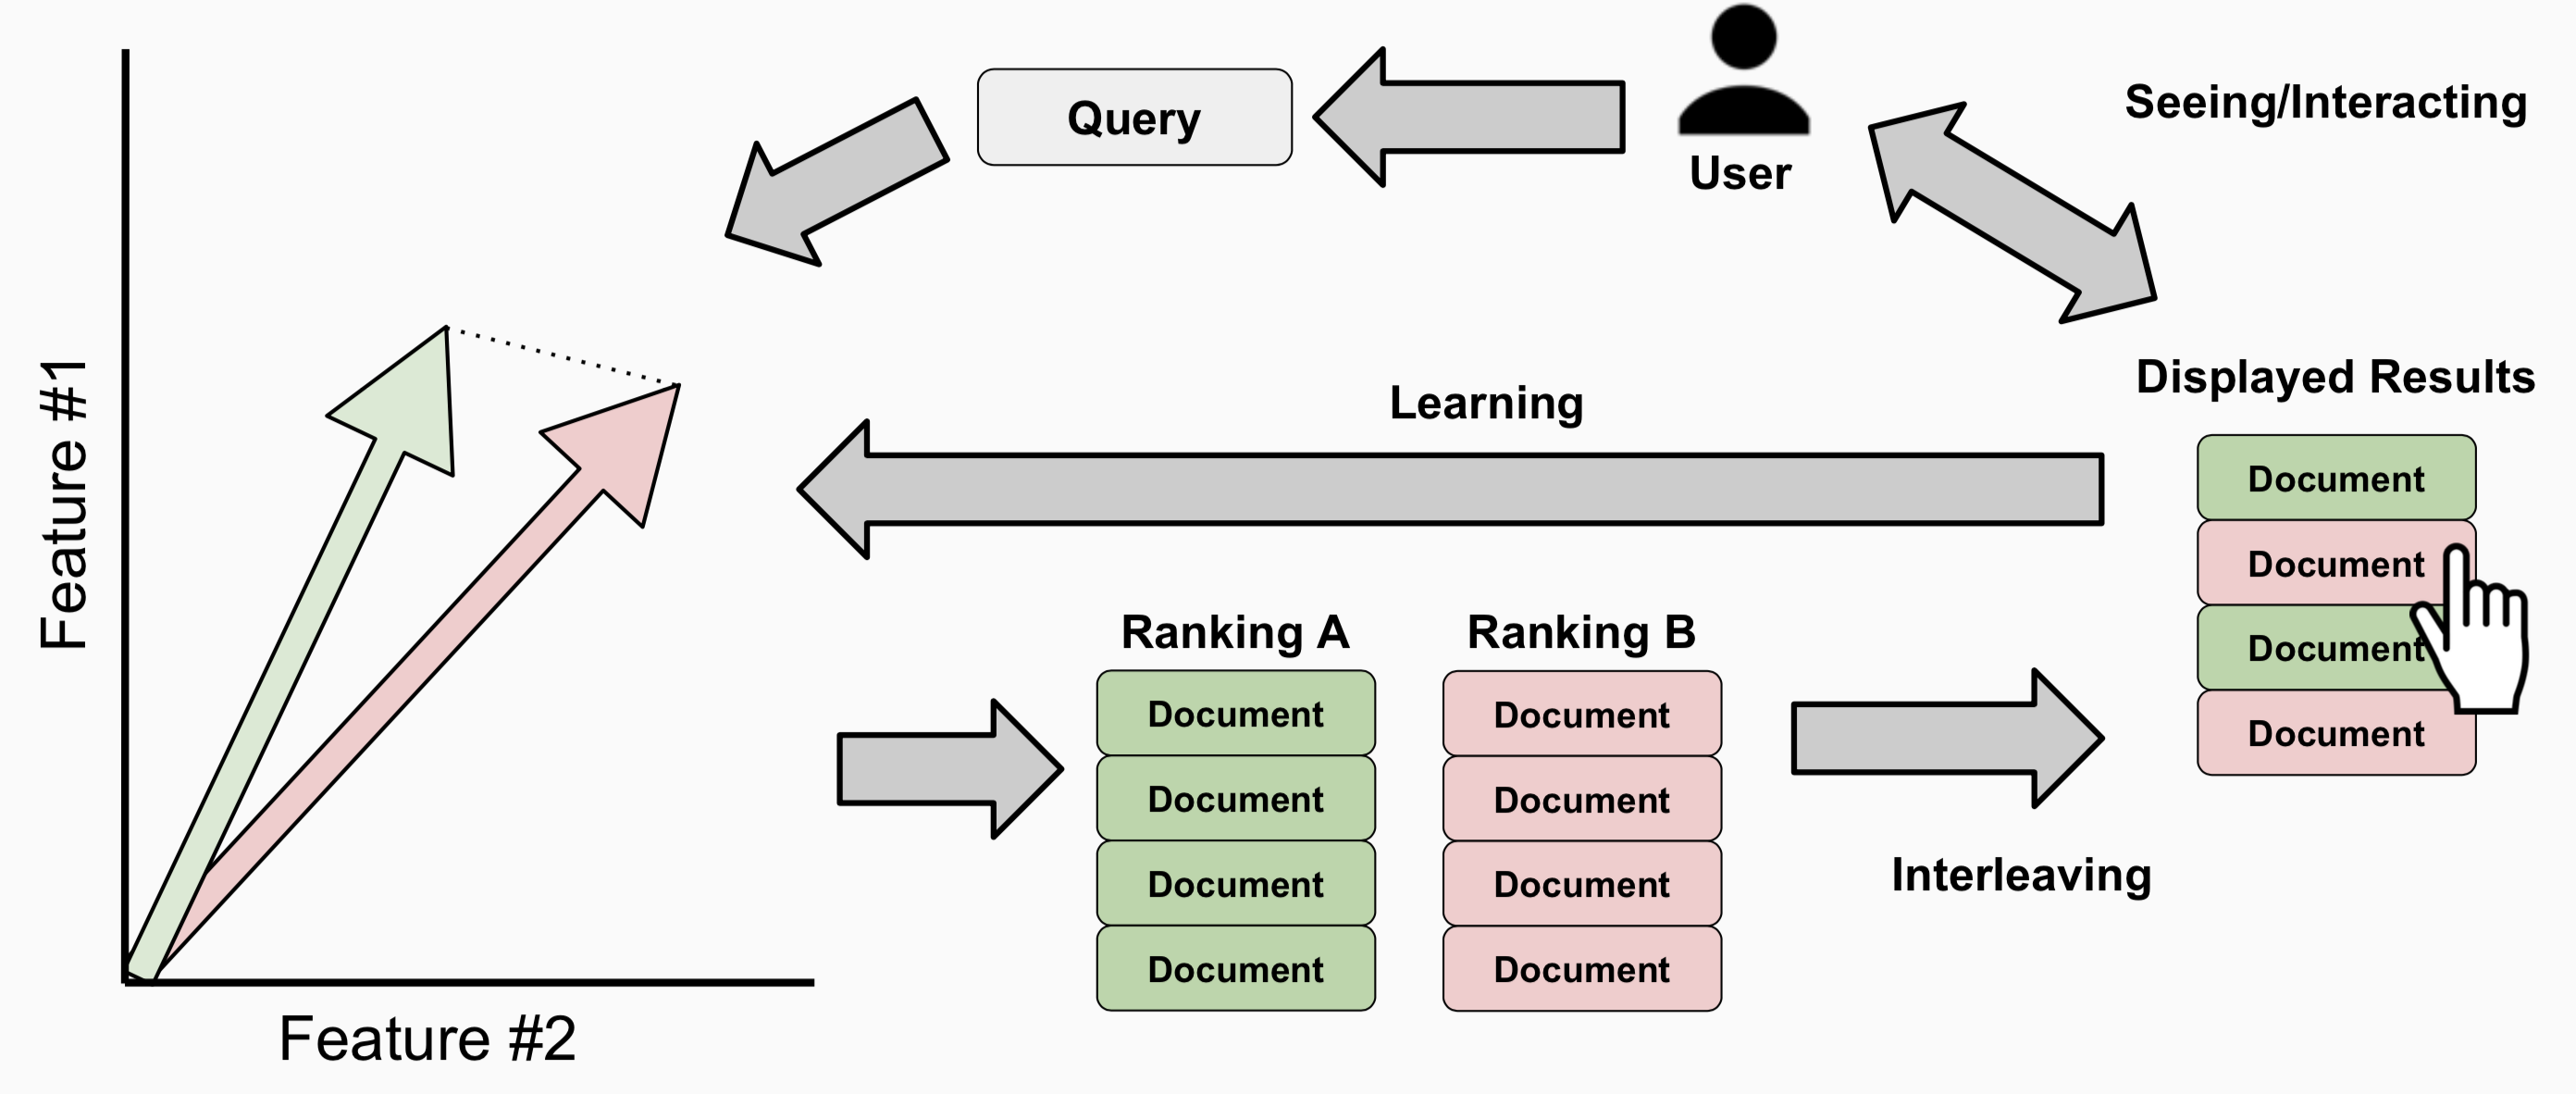
\includegraphics[width=0.5\textwidth]{figures/learning_to_rank_online_DBGD.png}
		\caption{Steps in Dueling Bandit Gradient Descent}
		\label{img:learning_to_rank_online_DBGD}
	\end{figure}
	\item It can be shown that if there is only a single optimum, the Dueling Bandit Gradient Descent algorithm will be able to approximate the optimal model
\end{itemize}
\section{Counterfactual Evaluation and Learning to Rank}
\begin{itemize}
	\item The term \textit{counterfactual} relates to \textit{off-policy} learning in RL
	\item Thus, we try to evaluate an offline task by using online data obtained by another policy to estimate the performance of the new policy in a online setting
\end{itemize}
\subsection{Counterfactual Evaluation}
\begin{itemize}
	\item In general, a user interactive system can be formalized as follows (see Figure~\ref{img:counterfactual_user_interactive_system}):
	\begin{itemize}
		\item $x$: Feature vector describing the user and context (i.e. query)
		\item $y$: Result the system returns based on its policy ($y=\pi(x)$)
		\item $\delta$: Feedback signal from the actions a user took. The function encodes the metric (user utility function) and is defined as $\delta: X\times Y\to \mathbb{R}$
		\item $\pi$: Policy describing the ranking system which takes $x$ as input and maps it to output $y$: $\pi:X\to Y$
	\end{itemize}
	\begin{figure}[ht]
		\centering
		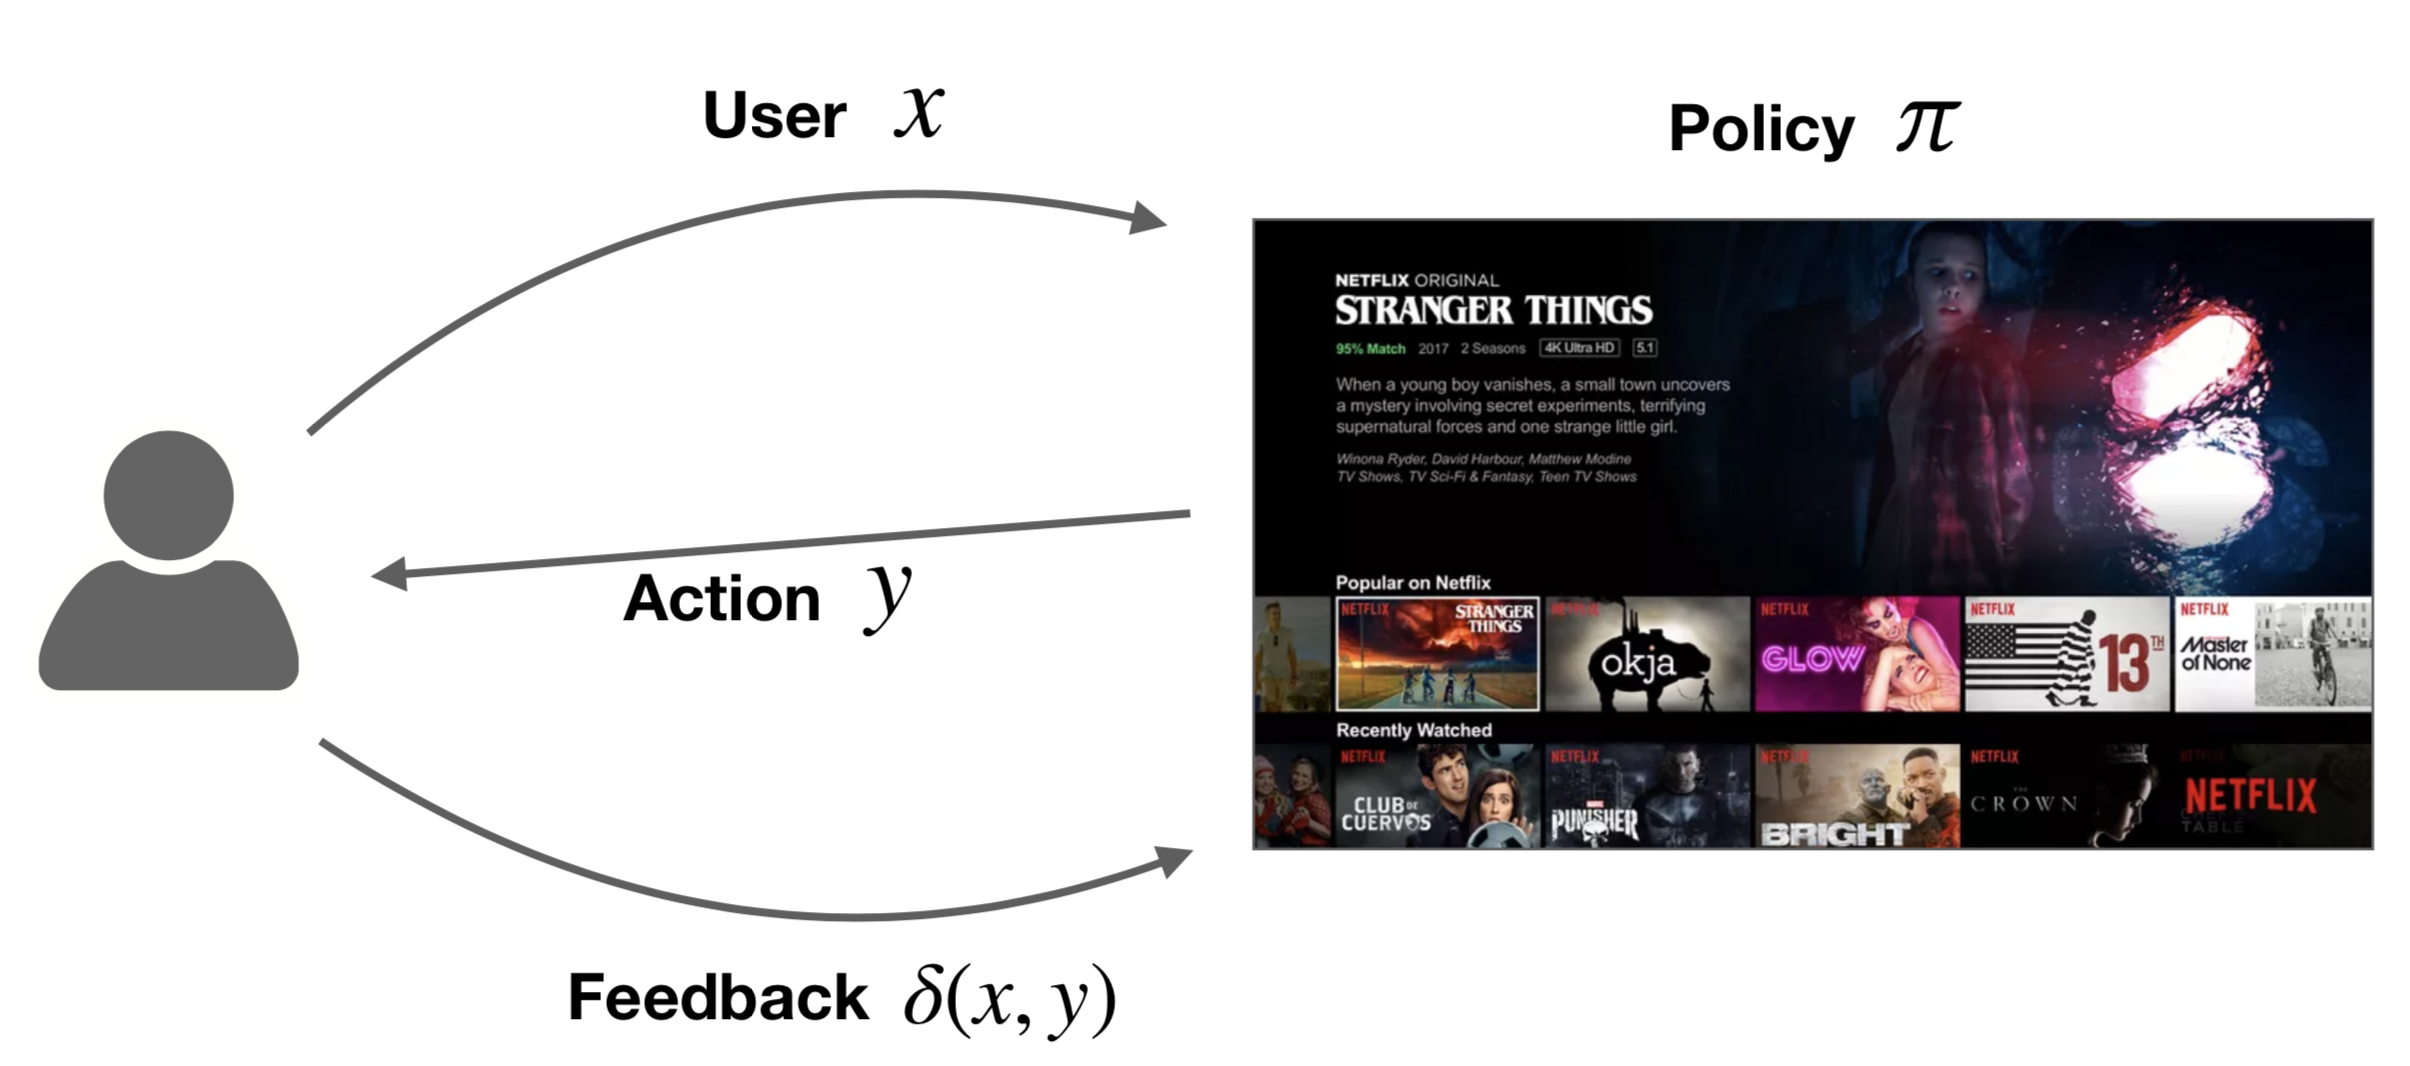
\includegraphics[width=0.5\textwidth]{figures/counterfactual_user_interactive_system.png}
		\caption{Visualization fo a user interactive system}
		\label{img:counterfactual_user_interactive_system}
	\end{figure}
	\item \textit{Counterfactual evaluation}: perform offline evaluation of online metrics given online data from another system $\pi_{\text{production}}$. Thus, we try to estimate performance of $\pi_{\text{new}}$ with interaction data obtained with $\pi_{\text{production}}$.
	\item The interactions data/log is structured as $D=\left\{\left(x_1, y_1, \delta_1\right),...,\left(x_n, y_n, \delta_n\right)\right\}$
	\begin{itemize}
		\item The actions $y_i$ were selected by $\pi_{\text{production}}:X\to Y$
		\item Note that we only have partial information feedback, and no complete supervision. Only for the chosen action, we know the feedback signal/user utility. Thus, the "correct"/optimal action is unknown (also called "bandit feedback" as it was sampled from only one arm)
	\end{itemize}
	\item We want to estimate $\mathbb{E}_{y\sim \pi_{\text{new}}}\left[\delta(x,y)\right]$ given $D$ from $\pi_{\text{production}}$. For this, there are two approaches: \textit{model the rewards} and \textit{inverse propensity scoring}.
\end{itemize}
\subsubsection{Model the rewards}
\begin{itemize}
	\item The intuition behind \textit{model the rewards} is to learn the reward function $\delta:X\times Y\to \mathbb{R}$ from $D\sim \pi_{\text{production}}$ directly
	\item The task can be reduced to a regression problem: $$\delta_w = \arg\min_{\delta_w} \sum\limits_{i=1}^{N} \mathcal{L}\left(\delta_w\left(x_i, y_i\right), \delta_i \right)$$
	where $\mathcal{L}$ is a loss function like MSE.
	\item Once $\delta_w$ is learned, we can estimate our goal by $\mathbb{E}_{y\sim \pi_{\text{new}}}\left[\delta(x,y)\right] = \frac{1}{n} \sum\limits_{i=1}^{N} \delta_w \left(x_i, \pi_{\text{new}}(x_i)\right)$
	\item However, learning $\delta_w$ is in general very difficult, as:
	\begin{itemize}
		\item Input space $X\times Y$ is very high-dimensional
		\item Rewards are highly non-linear and noisy
		\item Data is strongly biased to the actions that $\pi_{\text{production}}$ prefers
	\end{itemize}
\end{itemize}
\subsubsection{Inverse Propensity Scoring}
\begin{itemize}
	\item Instead of learning $\delta_w$, is it possible to directly estimate the value of the new policy $\pi_{\text{new}}$?
	\item Answer: only under the condition that the policy $\pi_{\text{production}}$ is stochastic: $y\sim \pi(y|x)$. The probability $p$ to choose the action $y$ is also called \textit{propensity}. Note that $p>0$ must hold for all possible actions as we otherwise have no chance to discover/obtain feedback for all actions
	\item For unbiased counterfactual evaluation, we need data samples with the propensity $p_i$ from policy $\pi_{\text{production}}$ describing the probability of selecting $y_i$ for given input $x_i$: $\left(x_i, y_i, \delta_i, p_i\right)$
	\item Use importance sampling to make distributions $\pi_{\text{production}}$ and $\pi_{\text{new}}$ comparable. This leads to the \textbf{IPS-estimator}:
	$$\frac{1}{n}\sum\limits_{i=1}^{N} \delta_i \frac{\pi_{\text{new}}(y_i|x_i)}{p_i}$$
\end{itemize}
\subsubsection{Proof of Unbiasedness}
\begin{itemize}
	\item We want to proof that in expectation, the IPS estimator will lead to the correct value: $$\mathbb{E}_{y\sim \pi_{\text{production}}}\left[\frac{1}{n}\sum\limits_{i=1}^{N} \delta_i \frac{\pi_{\text{new}}(y_i|x_i)}{p_i}\right] = \mathbb{E}_{y\sim \pi_{\text{new}}}\left[\delta(x,y)\right]$$
	\item First, we can put the sum outside the expectation:
	$$\mathbb{E}_{y\sim \pi_{\text{production}}}\left[\frac{1}{n}\sum\limits_{i=1}^{N} \delta_i \frac{\pi_{\text{new}}(y_i|x_i)}{p_i}\right] = \frac{1}{n}\sum\limits_{i=1}^{N} \mathbb{E}_{y\sim \pi_{\text{production}}}\left[\delta_i \frac{\pi_{\text{new}}(y_i|x_i)}{p_i}\right]$$
	\item Next, we replace the expectation by a sum over actions weighted by their corresponding probabilities:
	$$\frac{1}{n}\sum\limits_{i=1}^{N} \mathbb{E}_{y\sim \pi_{\text{production}}}\left[\delta_i \frac{\pi_{\text{new}}(y_i|x_i)}{p_i}\right] = \frac{1}{n}\sum\limits_{i=1}^{N} \sum\limits_{y_i\in Y}\left[\pi_{\text{production}}(y_i|x_i)\delta_i \frac{\pi_{\text{new}}(y_i|x_i)}{p_i}\right]$$
	\item As $p_i$ is defined as $\pi_{\text{production}}(y_i|x_i)$, we can reduce the equation to:
	$$\frac{1}{n}\sum\limits_{i=1}^{N} \sum\limits_{y_i\in Y}\left[\pi_{\text{production}}(y_i|x_i)\delta_i \frac{\pi_{\text{new}}(y_i|x_i)}{p_i}\right] = \frac{1}{n}\sum\limits_{i=1}^{N} \sum\limits_{y_i\in Y}\left[\delta_i \pi_{\text{new}}(y_i|x_i)\right]$$
	\item Finally, we apply rules based on the definition of expectation:
	$$\frac{1}{n}\sum\limits_{i=1}^{N} \sum\limits_{y_i\in Y}\left[\delta_i \pi_{\text{new}}(y_i|x_i)\right] = \frac{1}{n}\sum\limits_{i=1}^{N} \mathbb{E}_{y_i\sim \pi_{\text{new}}}\left[\delta(x_i,y_i)\right] = \mathbb{E}_{y\sim \pi_{\text{new}}}\left[\delta(x,y)\right]$$
	\item Note that the IPS estimator has a high variance which scales with $p_i^2$. Thus, if we have a very low probability for some actions, this can introduce a high error $\implies$ many samples needed to approximate target accurately. There are different approaches to reduce the variance
\end{itemize}
\subsection{Counterfactual Learning to Rank}
\begin{itemize}
	\item Learning to Rank: \textit{offline} - train on labeled data, \textit{online} - learn from user interactions, \textit{counterfactual} - learn offline from online retrieved data obtained by another policy/ranker
	\item The goal of counterfactual LTR is to learn a new ranker $\pi_{\text{new}}$ from the interaction data with $\pi_{\text{production}}$
	\begin{itemize}
		\item The data is specified by $D=\left\{(x_1,y_1,\delta_1),...,(x_N,y_N,\delta_N)\right\}$ where $\delta_i$ indicates which document was clicked (we assume that only one document was clicked)
		\item $y_i$ is the ranking selected by $\pi_{\text{production}}:X\to Y$
	\end{itemize}
	\item Naive approach: assume click indicates relevance and learn as if it would be a supervised dataset: $$\pi_{\text{new}} = \arg\min_{\pi} \sum\limits_{i=1}^{N} \text{rank}\left(\pi(x_i),y_i,\delta_i\right)$$
	The objective function is to reduce the rank of the relevant document given the new ranking of $\pi_{\text{new}}$ and the previous ranking by $y_i$. Can be solved by pairwise LTR objective.
	\item However, data obtained by online Learning to Rank is commonly noisy and biased
	\item We can take these biases into account by using the inverse propensity scores:
	$$\pi_{\text{new}} = \arg\min_{\pi} \sum\limits_{i=1}^{N} \frac{\text{rank}\left(\pi(x_i),y_i,\delta_i\right)}{p(\textit{observing }\delta_i)}$$
	This formula can be motivated from a probabilistic click model perspective:
	$$p(\textit{click}) = p(\textit{observation})\times p(\textit{relevant}) \implies p(\textit{relevant}) = \frac{p(\textit{click})}{p(\textit{observation})}$$
	Left side is what we want to get, and on the right side it is specified what we actually optimize.
\end{itemize}
\subsubsection{Propensity estimation}
\begin{itemize}
	\item However, the question remains how we calculate $p(\textit{observing }\delta_i)$. We can either approximate it by using click models, or by performing a randomization test
	\item \textit{RandTopN}
	\begin{itemize}
		\item Randomly shuffle the top $N$ documents
		\item Measure clicks people have performed on the data (online experiment)
		\item Aggregate clicks for infinite samples
		\item Infer $\hat{p} \propto p(\textit{observing} \delta_i)$
	\end{itemize} 
	\item \textit{RandPair}
	\begin{itemize}
		\item Randomly swap top document with random top $N$ documents
		\item Infers $\frac{p(\textit{observing} \delta_i)}{p(\textit{observing} \delta_j)}$ for swapped documents $i$ and $j$
	\end{itemize}
	\begin{figure}[ht]
		\centering
		\begin{subfigure}[b]{0.45\textwidth}
			\centering
			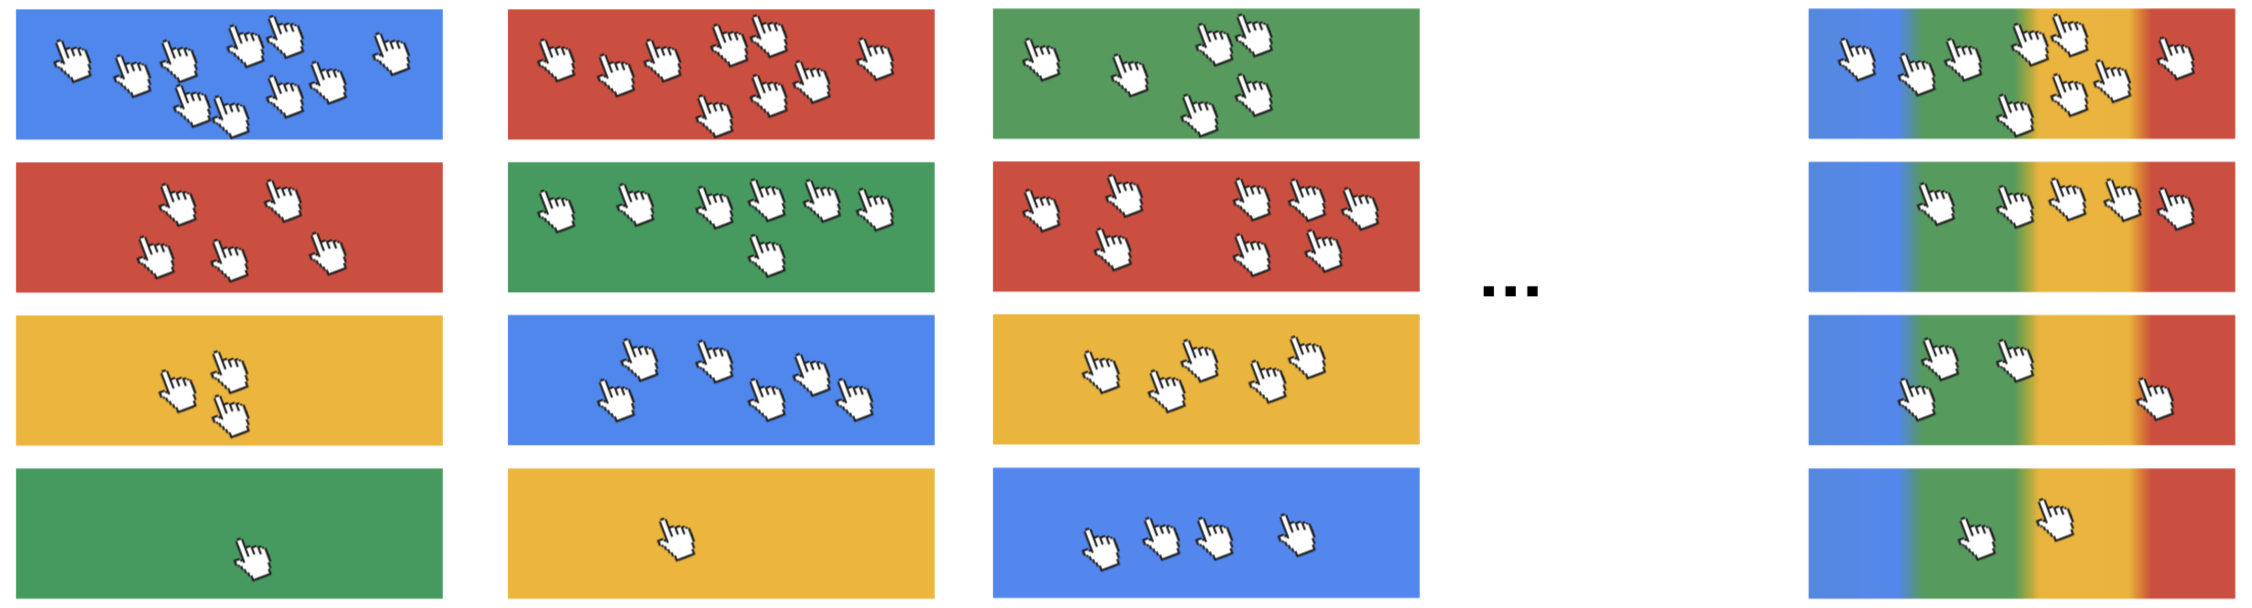
\includegraphics[width=0.8\textwidth]{figures/counterfactual_LTR_RandTopN.png}
			\caption{RandTopN}
		\end{subfigure}
		\begin{subfigure}[b]{0.45\textwidth}
			\centering
			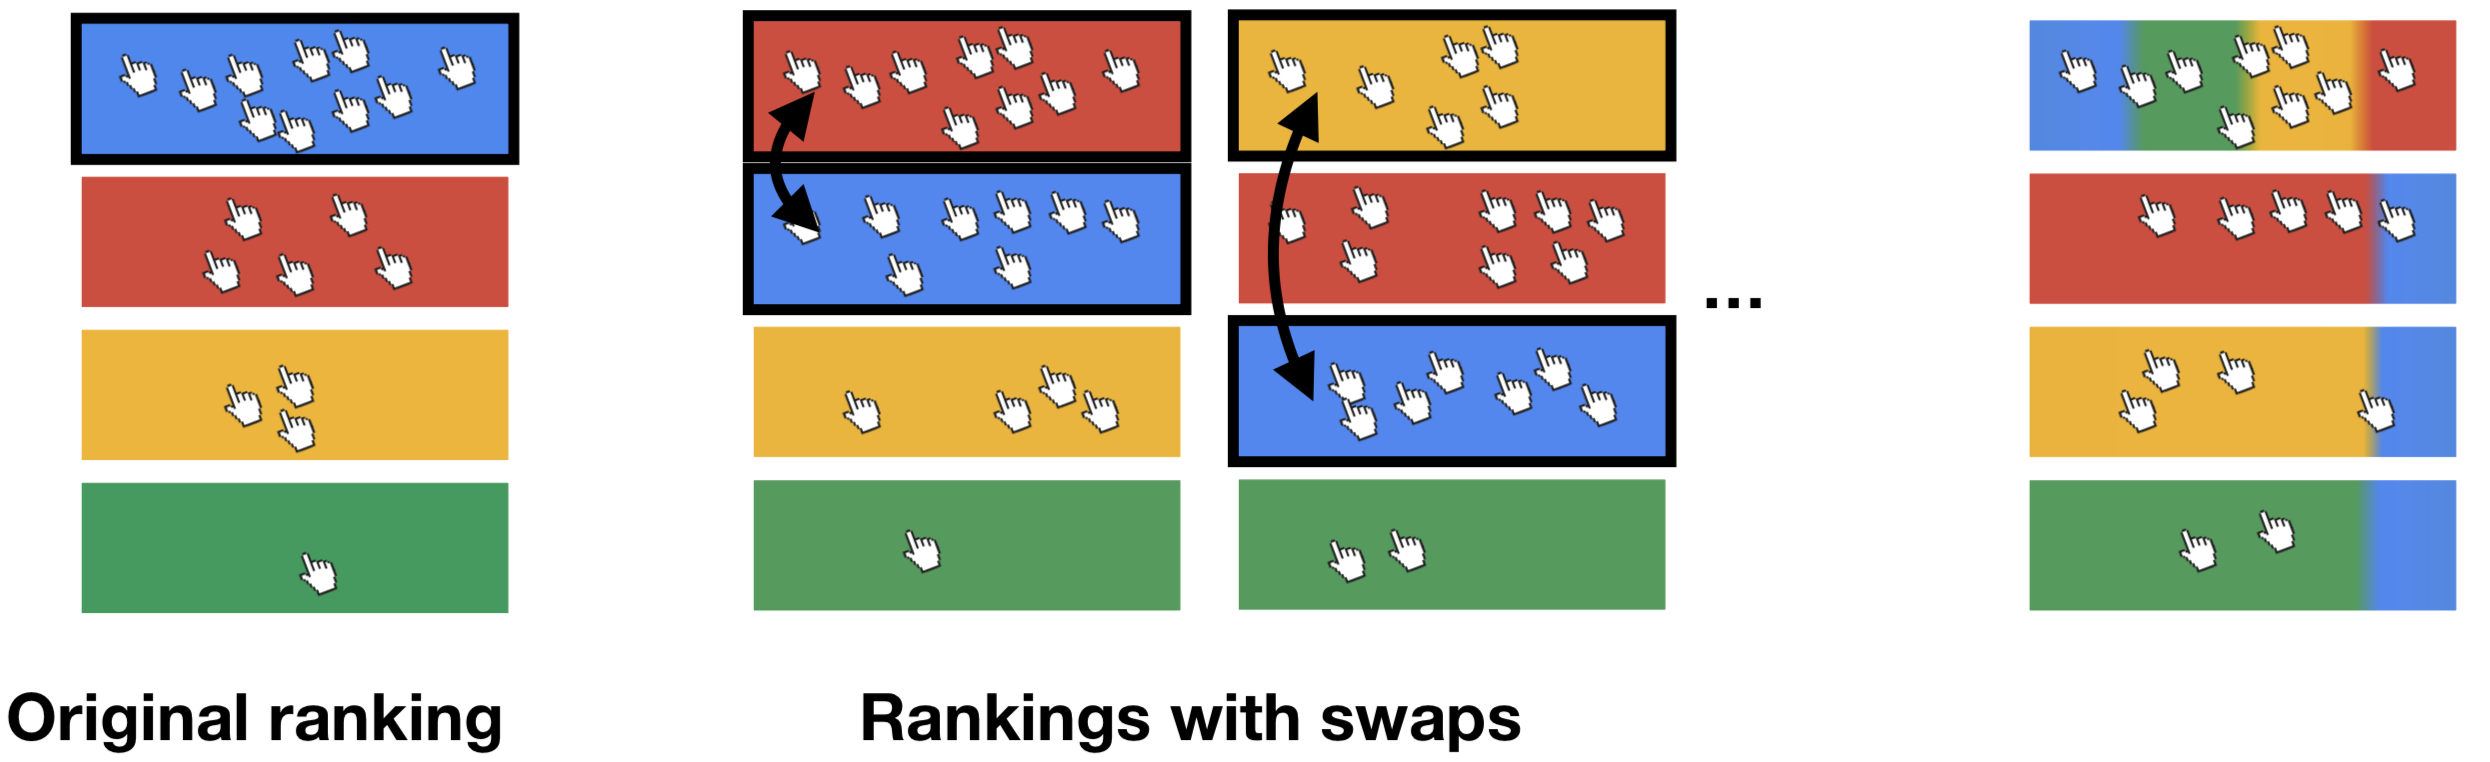
\includegraphics[width=0.8\textwidth]{figures/counterfactual_LTR_RandPair.png}
			\caption{RandPair}
		\end{subfigure}
		\label{img:counterfactual_propensity_estimation}
	\end{figure}
\end{itemize}
\subsubsection{The Variance problem}
\begin{itemize}
	\item The problem of solving the counterfactual approach is that if $p(\textit{observing} \delta_i)$ heads to $0$, the overall objective will be heavily biased towards this example $\implies$ overfitting on single data point
	\item One way to overcome this problem is using a variance regularizer which prevents the policy to deviate too much from the original production policy $\pi_{\text{production}}$:
	$$\pi_{\text{new}} = \arg\min_{\pi} \sum\limits_{i=1}^{N} \frac{\text{rank}\left(\pi(x_i),y_i,\delta_i\right)}{p(\textit{observing }\delta_i)} + \lambda \sqrt{\frac{\mathcal{V}[\pi, \pi_{\text{production}}]}{n}}$$
	\item However, this optimization problem cannot be solved by SGD anymore and iterative methods must be applied (new learning framework \textit{counterfactual risk minimization})
\end{itemize}
\appendix
% \newpage
% \input{nlp_appendix.tex}
\end{document}